\documentclass[titlepage, openright, letterpaper, 12pt]{book}
\usepackage{entete,commandes} % Load les packages et définit des commandes.

%=============================================================================%

% \makeatletter
%     \newcommand{\showfont}{
%         \begin{itemize}
%             \item encoding: \f@encoding{}
%             \item family: \f@family{}
%             \item series: \f@series{}
%             \item shape: \f@shape{}
%             \item size: \f@size{}
%         \end{itemize}
%     }
% \makeatother
% \showfont

% On crée des bools qui sont False par défaut.
\newtoggle{VersionLivre}
\newtoggle{LivrePGChVide}
\newtoggle{ForceEntete}
\newtoggle{AuteureFemme}
\newtoggle{MemoirePasThese}
\newtoggle{useCustomFonts}
\newtoggle{generatePDFa}
\newtoggle{IntroConcluSansNombre}

% Switchboard, l'endroit ou on ajuste les toggles.
% Décommenté -> True; commenté -> False

%\toggletrue{VersionLivre}          % Décommenter pour faire la version livre
%\toggletrue{LivrePGChVide}         % Page gauche de chapiter vide en mode livre.
%\toggletrue{ForceEntete}            % Entête même pour version électronique.
%\toggletrue{AuteureFemme}          % Décommenter si l'auteur est une femme.
\toggletrue{MemoirePasThese}       % Décommenter dans le cas d'un mémoire.
\toggletrue{IntroConcluSansNombre}  % Intro et conclusion non numérotées
\toggletrue{useCustomFonts}         % Fonts différents, voir switchboard.tex.
%\toggletrue{generatePDFa}           % Génère un PDFa plutôt qu'un PDF standard.

%=============================================================================%

\title          {TenSAT: Optimisation de la résolution des modèles $p$-spin avec les réseaux de tenseurs} % Les réseaux de tenseurs pour les modèles $p$-spin% Pour la page de titre/jury.
\author         {Benjamin Lanthier}  % Idem
\Organisation   {UNIVERSITÉ de SHERBROOKE}
\Location       {Sherbrooke, Québec, Canada}
\ResumeCourt    {On présente des résultats nouveaux dans un domaine en pleine effervescence.}
\date           {\today}       % Idem
\MotsClefs      {Mots-Clefs \sep Pertinents \sep avec séparateurs}

% On cache le code exécuté dans ce fichier parce qu'il est laid et impertinent.
\begin{comment}
\end{comment}

%=============================================================================%

\makeatletter   % Permet d'accèder aux variables @

%=============================================================================%

    % PDFA-1b/Hyperref
    \iftoggle{generatePDFa}
    {
        % PDF/A stuff (experimental)
        \usepackage[a-1b]{pdfx}
    }
    {
        \newcommand{\sep}{, }
    }
        \usepackage{filecontents}
        \begin{filecontents*}{\jobname.xmpdata}
                \Title          {\@title}
                \Author         {\@author}
                \Subject        {\ResumeCourt}
                \Org            {\Organisation}
                \Keywords       {\MotsClefs}
                \PublicationType{book}
        \end{filecontents*}
        % Couleurs moins intenses, https://ethanschoonover.com/solarized/
        \definecolor{solblue}{HTML}{268bd2}
        \definecolor{solred}{HTML}{dc322f}
        \definecolor{solviolet}{HTML}{6c71c4}
        \definecolor{solmagenta}{HTML}{d33682}
        \definecolor{solcyan}{HTML}{2aa198}
        \definecolor{solorange}{HTML}{cb4b16}
        \definecolor{solyellow}{HTML}{b58900}
        \definecolor{solgreen}{HTML}{859900}
        % Hyperrefs
        \usepackage{hyperref}
        \hypersetup{
            pdfauthor={\@author},
            pdftitle={\@title},
            pdfsubject={\ResumeCourt},
            pdfkeywords={\MotsClefs},
            hyperindex=true,
            bookmarks=true,
            pdfa,
            %pdftex,
            colorlinks=true,
            breaklinks=true,
            urlcolor=solmagenta,
            %linkcolor=solblue!85!black, % A little darker
            linkcolor=solblue,
            citecolor=solcyan,
            bookmarksopen=true,
            unicode=true
        }
        \usepackage[hyperpageref]{backref}      % Backrefs!
        \renewcommand{\backref}[1]{[cf.~p.~#1]} % Volé cette ligne à Samuel Boutin
        \usepackage{bookmark}
        \usepackage{cmap} % Doit être après hyperref pour être compatible avec pdf-a

%=============================================================================%

    \iftoggle{useCustomFonts}
    {   
        % Deux prochaines lignes -> Pagella et Mathpazo
        %\usepackage{mathpazo} % utilise Palatino pour les mathématiques (mettre en premier)
        %\usepackage{tgpagella} % utilise la police TeX Gyre Pagella

        % Deux prochaines lignes -> New Century et Fourier
        %\usepackage{newcent}
        %\usepackage{fouriernc}
        
        \usepackage{newcent}
        \usepackage{fouriernc}
        \renewcommand{\dagger}{\text{\textdagger}} % Millennial missing dagger fix
        \renewcommand{\iint}{\int\!\!\int}  % Better spacing
        \renewcommand{\iiint}{\int\!\!\int\!\!\int}
        \renewcommand{\iiiint}{\int\!\!\int\!\!\int\!\!\int}
    }
    {}

%=============================================================================%
    
    \iftoggle{AuteureFemme}
    { \newcommand{\monsieurMadame}{Mme.} }    
    { \newcommand{\monsieurMadame}{M.} }

%=============================================================================%

    \iftoggle{MemoirePasThese}
    {   % Si c'est un mémoire
        \newcommand{\documentPresente}{Mémoire présenté}
        \newcommand{\leDocument}{le mémoire}
        \newcommand{\leGrade}{maître ès science (M.Sc.)}
    }
    {   % Si c'est une thèse
        \newcommand{\documentPresente}{Thèse présentée}
        \newcommand{\leDocument}{la thèse}
        \newcommand{\leGrade}{docteur ès science (Ph.D.)}
    }

%=============================================================================%
    
    % Gestion de la version électronmique vs celle imprimée.
    \iftoggle{VersionLivre}
    {   % On fait la version imprimée!

        % On utilise un fontsize plus petit(10pt vs 12pt).
        \let\small\relax
        \let\footnotesize\relax
        \let\scriptsize\relax
        \let\tiny\relax
        \let\large\relax
        \let\Large\relax
        \let\LARGE\relax
        \let\huge\relax
        \let\Huge\relax
        \input{size10.clo}  % Ajuste le fontsize ET les marges
        \geometry{twoside=true, bottom=2.54cm} % L'ordre est important, pour les marges/fontsize.
        %\widowpenalty5000  % Décommenter s'il y a trop de ligne veuves/orphelines.
        %\clubpenalty5000   


        % On enlève la numérotation des pages vides
        \let\origdoublepage\cleardoublepage
        \newcommand{\clearemptydoublepage}{%
            \clearpage%
            {\pagestyle{empty}\origdoublepage}%
            }
        \let\cleardoublepage\clearemptydoublepage
        
        % Permet de mettre un page blanche seulement dans la version imprimée
        \newcommand{\autoPageBlancheLivre}{\clearpage\null\thispagestyle{empty}}

        \iftoggle{LivrePGChVide}
        {
            \let\stdchapter\chapter
            \renewcommand\chapter{\clearpage\null\thispagestyle{empty}\stdchapter}
            \renewcommand{\autoPageBlancheLivre}{}

            \let\stdpart\part
            \renewcommand\part{\clearpage\null\thispagestyle{empty}\stdpart}

            \renewcommand\@endpart{\vfil
                          \if@twoside
                            \null
                            \thispagestyle{empty}%
                            \newpage
                          \fi
                          \if@tempswa
                            \twocolumn
                          \fi}
        }{}

        % Les hyperliens n'ont pas desoins d'être colorés
        \hypersetup{hidelinks}
        % On affiche les DOI dans la biblio -> Pratique en version imprimée
        \bibliographystyle{nature-fr-showdoi}
        % On garde les entêtes dans la bibliographie
        \newcommand{\bibpagestyle}{}
    }
    {   % S'il y a un côté, on fait la version électronique.
        \geometry{letterpaper, lmargin=1.25in, rmargin=1.25in,
                  tmargin=1.5in, bmargin=1.0in, twoside=false}
        \iftoggle{ForceEntete}
        {
            % On garde les entêtes dans la bibliographie
            \newcommand{\bibpagestyle}{}
        }
        {
        % Prochaines lignes enlèvent l'entête
            \renewcommand{\chaptermark}[1]
                {\markboth{{\thechapter. #1}}{}}
            \renewcommand{\sectionmark}[1]{}
            % On enlève les entêtes dans la bibliographie
            \newcommand{\bibpagestyle}{\pagestyle{plain}}
        }

        % On n'affiche pas les DOI dans la biblio -> Plus propre
        \bibliographystyle{nature-fr}
        %\bibliographystyle{unsrt-fr} % unsrt partiellement traduit. Préférer nature.
        
        % Permet de mettre un page blanche seulement dans la version imprimée
        \newcommand{\autoPageBlancheLivre}{}
    }
    \iftoggle{IntroConcluSansNombre}
    {
        \newcommand{\Introduction}{\chapter*{Introduction}
            \addcontentsline{toc}{chapter}{Introduction}}
        \newcommand{\Conclusion}{\chapter*{Conclusion}
            \addcontentsline{toc}{chapter}{Conclusion}}
    }
    {
        \newcommand{\Introduction}{\chapter{Introduction}}
        \newcommand{\Conclusion}{\chapter{Conclusion}}
    }


%=============================================================================%

\makeatother    % Plus d'accès aux variables @


%=============================================================================%

\begin{document}

%=============================================================================%
% Titre
\begin{comment}
\end{comment}
\makeatletter   % Permet d'accèder aux variables @

\thispagestyle{empty}  % Page blanche avec formattage manuel
\pagenumbering{gobble} % Aucune numérotation, sinon hypperref bug
\vglue 2cm
\begin{center}
    \doublespacing{
    {\LARGE \@title}\\
    \vspace{2.0cm}
    par\\
    \vspace{2.0cm}
    {\large \@author}
    \vspace{2.0cm}\\
    \documentPresente\ au département de physique\\
    en vue de l'obtention du grade de \leGrade
    \vfill
    FACULTÉ des SCIENCES\\
    \Organisation\vspace{1.0cm}\\
    \Location, \@date  % La date sera celle de la compilation
    }
\end{center}

\makeatother    % Plus d'accès aux variables @


\frontmatter % Pagination de préambule

% Jury
\begin{comment}
\end{comment}
\makeatletter   % Permet d'accèder aux variables @

\iftoggle{LivrePGChVide}
{}
{
    % Next two lines force a linebreak in ebook versions
    \chapter*{}
    \vspace{-4.7cm}
}

\thispagestyle{empty}

\begin{center}
    \vglue 2cm
    Le \underline{\hspace{5cm}}\\ 
    % Le \@date % Lorsque le document sera accepté!
    \vspace{2cm}
    \scalebox{1} % Empêche le retour à la ligne si le nom est trop long.
    % {\it le jury a accepté \leDocument\ de \monsieurMadame~\@author~dans sa version finale.} 
    
    \vspace{2cm}
    Membres du jury\\
    \vspace{2cm}

    Professeur Stefanos Kourtis\\
    Directeur de recherche\\
    Département de physique\\
    \vspace{2cm}
    
    Professeur Eva Dupont-Ferrier\\
    Membre interne\\
    Département de physique\\
    \vspace{2cm}

    Professeur David Sénéchal\\
    Président rapporteur\\
    Département de physique\\
    \vspace{2cm}
\end{center}

%\clearpage

\makeatother    % Plus d'accès aux variables @


% Dédicace
\begin{comment}
\end{comment}

\chapter*{}
\vspace{-10pt}
\begin{flushright}
    << One often meets his destiny on the road he takes to avoid it.>>

    \emph{-- Maître Oogway}
\end{flushright}

\thispagestyle{empty}

% Sommaire
\clearpage  % Mets le sommaire à la bonne page dans la TOC
\chapter*{Résumé}
\addcontentsline{toc}{chapter}{Résumé}
\begin{comment}
\end{comment}

Bref résumé.
% We introduce a tensor network algorithm for the solution of $p$-spin models.
% We show that bond compression through rank-revealing decompositions performed during the tensor network contraction resolves logical redundancies in the system exactly and is thus lossless, yet leads to qualitative changes in runtime scaling in different regimes of the model.
% First, we find that bond compression emulates the so-called leaf-removal algorithm, solving the problem efficiently in the ``easy'' phase.
% Past a dynamical phase transition, we observe superpolynomial runtimes, reflecting the appearance of a core component.
% We then develop a graphical method to study the scaling of contraction for a minimal ensemble of core-only instances, for which leaf removal is ineffective.
% We find subexponential scaling, improving on the exponential scaling that occurs without compression.
% Our results suggest that our tensor network algorithm subsumes the classical leaf removal algorithm and simplifies redundancies in the $p$-spin model through lossless compression, all without explicit knowledge of the problem's structure.




% Remerciements
\chapter*{Remerciements}
\begin{comment}
\end{comment}

% Merci!

Je voudrais commencer par remercier Stefanos pour m'avoir accepté dans son groupe de recherche qui, à prime abord, ne semble pas trop connecté avec mes études en ingénierie physique.
Tu m'as donné un projet super intéressant, mais tu as aussi su être un excellent guide tout au long de mon parcours.
Merci pour ta patience et pour m'avoir mis en confiance, tant avec les connaissances théoriques requises pour ce projet qu'avec tes conseils au niveau du code.

Merci à Jeremy pour ton aide précieuse tout au long de ce projet, tu as su être un excellent mentor et ton implication a été grandement appréciée.
Tu as toujours été disponible pour répondre à mes questions, peu importe leur niveau de difficulté, mais aussi pour nos discussions sur nos objectifs et motivations.
Ça m'a fait grand plaisir!
Merci aussi à tous les membres du groupe pour votre aide, votre écoute, mais aussi pour les moments que nous avons partagés et les liens que nous avons formés.
Que ce soit les parties de rugby dehors pendant l'été, les séances de frisbee, ou les conférences, nous avons su créer une belle ambiance qui a aidé à alléger la pression sur nos épaules, et j'en suis très reconnaissant.
Je suis chanceux d'être tombé dans un groupe avec une ambiance comme la nôtre.

Je tiens maintenant à remercier toute ma famille pour vos encouragements ainsi que votre soutien constant.
Vous apportez toujours de la joie dans mes journées lorsque nous sommes ensemble, et je vous en serai éternellement reconnaissant!

Un grand merci à tous mes amis qui, par un heureux hasard à la Polytechnique, se sont retrouvés dans le même bateau que moi pendant ces deux années.
Béatrice, Dominic, Jonathan, Marie-Frédérique, Thomas, Thomas et Simon; vous avez été une source de connaissances, de motivation, de niaiseries et de sorties — bref, vous avez rendu ces années mémorables!
Je suis particulièrement reconnaissant que \textit{niaiseries} et \textit{sorties} soient au pluriel dans cette phrase, car tous ces moments ont égayé des journées qui, par moments, pouvaient sembler plus grises pendant cette période de recherche.
Un merci tout spécial à Laurence (et son Léo) pour ton support incroyable, ta patience et ta bonne humeur contagieuse!
Tu m'as motivé et encouragé dans des moments plus difficiles et ça, je t'en suis redevable!

Finalement, je voudrais remercier, de manière générale, tous ceux que j'aime!
Sans vous, je ne pense pas que je serais rendu où je suis en ce moment.
Vous avez été les phares qui m'ont guidé à travers le brouillard de ces deux années de maîtrise, mais aussi le Soleil qui me permettait d'entrevoir la fin de ce projet.

% Julien, Martin, Antoine, Pierre-Alexandre, Jérémie et j'en passe pour m'avoir écouté et aidé lors des passages plus difficiles, mais aussi pour tous les moments qu'on a passés ensemble.
% Que ce soit les parties de rugby dehors durant l'été, les séances de frisbee ou les soirées un peu plus arosées, on a su créer une belle ambiance entre nous qui aide à baisser la pression qui nous est mise sur les épaules et j'en suis tr;s reconnaissant.

% Évidemment, un grand merci à Stefanos pour m'avoir parlé de ce projet qui a grandement piqué ma curiosité au début de la maîtrise et de m'avoir partagé ses connaissances sur les sujets qui se retrouvent dans ce projet.
% La première fois que je suis allé à l'UdS, c'était avec des amis pour voir les sujets de recherche des professeurs en physique.
% Je ne me doutais pas du tout que j'allais trouvé un groupe de recherche qui m'intéresse, encore moins qu'il m'intéresse assez pour m'inscrire à une maîtrise, mais me voici!
% Sa présentation sur l'utilisation de méthodes développées pour la physique qui peuvent être utilisées dans d'autres domaines scientifiques a piqué ma curiosité.

% Maintenant, je tiens à remercier tous mes amis de Poly --- MF, Doom, Tom, Jo et Simon ---, des personnes incroyables avec qui tout peut être un sujet de dicsussion, tant la physique que les sujets les plus randoms comme les pénis quantiques.
% Sans vous, ce deux ans auraient paru beaucoup plus long qu'il ne l'était vraiment!

% J'ai aussi un merci spécial pour toutes les merveilleuses personnes que j'ai rencontrées à l'université; Ben, Étienne, Luca, Julien, Émile.

% Pour finir, je tiens à remercier toute ma famille pour m'avoir soutenu et encouragé durant ce parcours.
% Votre constant soutient ainsi que vos encouragements sont ce qui m'a permis de pousser plus loin même lorsque la montagne semblait trop haute!
% Aussi, discuter des sujets qui se trouvent dans mon projet avec vous et vous voir vous informer pour essayer de me suivre lorsque vous me demandiez ce sur quoi je travaille, ça a été un vrai plaisir!% Vos tentatives d'écoutes de mon projet me touchent et, sincèrement, vous m'avez aidé à régler certains de mes problèmes alors vous m'avez permis d'avancer!




% Tables des matières/Figures
{
    \setlength{\parskip}{0ex}
    \tableofcontents
    \listoffigures
    %\listoftables
}

%=============================================================================%

\mainmatter % Pagination standard
\onehalfspacing

%-----------------------------------------------------------------------------%

% \include serait préférable à \input à partir d'ici, mais MiKTeX sur Windows
% n'aime pas les \cite dans un \include. Fonctionne parfaitement sur TeXLive.

\begin{comment}
\end{comment}

\Introduction   % Chapitre qui ne sera pas numéroté si IntroConcluSansNombre est Vrai

%-----------------------------------------------------------------------------%
Les verres de spin sont une classe de matériaux magnétiques caractérisés par leurs interactions désordonnées et frustrées entre les moments magnétiques individuels (spins)~\cite{stein2013spin}.
Contrairement aux ferromagnétiques ou aux antiferromagnétiques traditionnels où les spins s'alignent de manière uniforme, les verres de spin en présentent un arrangement complexe et aléatoire.
De nos jours, la physique des verres de spins se retrouve dans des domaines qui sont assez éloignés de son domaine d'origine, la matière condensée, comme dans l'informatique théorique~\cite{kirkpatrick1985configuration}, la biologie~\cite{bryngelson1987spin}, l'apprentissage machine~\cite{venkataraman1991spin} et même la planification des horaires pour les compagnies en aviation~\cite{stein2013spin}.
Les modèles de ces systèmes physiques sont, de manière générale, faciles à décrire, mais difficile à résoudre, donc difficile de trouver un état fondamental.
La principale explication de ce défi est que ces modèles présentent des paysages énergétiques qui ont une allure accidentée~\cite{stein2013spin, qing2009energylandscape}, ce qui coince les algorithmes d'optimisation dans des minimums locaux et cause un temps de résolution exponentiellement long.

Un contre-exemple de ces modèles est le $p$-spin~\cite{mezard_alternative_2002}, qui est en fait facilement résolvable même s'il possède le même genre de paysage énergétique que les autres modèles dans certains régimes de paramètres.
Effectivement, les systèmes modélisés par ce modèle peuvent se traduire en un système d'équations linéaires modulo $2$ et l'élimination gaussienne classique nous permet d'obtenir la fonction de partition du système à température nulle dans un temps polynomial.
Même si ce modèle est une version restreinte d'un modèle général de verre de spin, son analyse fournit des informations utiles sur la physique des verres de spin.
Comme il montre le même genre d'évolution énergétique en fonction des combinaisons de spins possibles et qu'il est simple à résoudre, il est aussi une référence standard pour les algorithmes classiques~\cite{bernaschi2021we, kanao2022simulated, aadit2023all} et quantiques~\cite{jorg2010first, farhi2012performance, hen2019equation, bellitti2021entropic, kowalsky20223, patil_obstacles_2019}.
Dans les régimes dans lesquels ce modèle possède le même genre de paysage énergétique, le recuit simulé n'est pas efficace, ou échoue, pour les systèmes pour lequel $p > 2$~\cite{patil_obstacles_2019, bellitti2021entropic} et c'est aussi vrai pour la méthode de recuit simulé quantique~\cite{farhi2012performance} même si aucune transition de phase n'est rencontrée~\cite{patil_obstacles_2019}.
La satisfiabilité booléenne et même les serveurs locaux ont de la difficulté avec ces modèles~\cite{haanpaa2006hard, jarvisalo2006further,jia2004spin, barthel2002hiding, ricci2001simplest, guidetti2011complexity}.

Ce mémoire introduit une méthode qui permet de résoudre les modèles $p$-spin en utilisant la satisfiabilité booléenne ainsi que les réseaux de tenseurs.
Les réseaux de tenseurs sont une structure de donnée qui permet une représentation compacte d'un modèle graphique (pondéré ou non), comme les Hamiltoniens de spin et les problèmes de satisfaction de contraintes, qui reviennent à compter le nombre de solutions au problème donné~\cite{garcia-saez_exact_2011, biamonte2015tensor, kourtis_fast_2019, Meichanetzidis_2019, de_beaudrap_tensor_2021}.
Bien que la contraction de réseaux de tenseurs soit, de manière générale, numériquement difficile même pour des classes de graphes restreintes comme les grilles planaires~\cite{schuch2007computational}, les techniques impliquant la compression de tenseur peuvent conduire à un résultat approximatif précis des fonctions de partition classiques ou des valeurs moyennes en mécanique quantiques (dans des cas spécifiques) de manière efficace.
Les réseaux de tenseurs ont aussi été utilisés dans des études de champs moyens de modèles graphiques et d'Hamiltonien de spin~\cite{alkabetz2021tensor, pancotti2023one}.

Dans la partie~\ref{part:theory} sur la théorie, les verres de spin ainsi que le modèle $p$-spin sont présentés dans les sections~\ref{sec:spin-glass} et~\ref{sec:p-spin} respectivement.
Elles sont ensuite suivies par une introduction sur la satisfiabilité booléenne à la section~\ref{sec:def-SAT} et par la définition du problème général \#$k$-XORSAT, qui permet la traduction d'un système $p$-spin à ce problème fondamental en informatique théorique, à la section~\ref{sec:k-xorsat}.
Les réseaux de tenseurs finissent ensuite le bal au chapitre~\ref{ch:TN}, où cet outil numérique ainsi que certaines de ses méthodes sont présentées.
Ensuite, la partie~\ref{part:methodology} sur la méthodologie explique comment relier le problème de satisfiabilité aux réseaux de tenseurs à la section~\ref{sec:tn-for-p-xorsat} et comment optimiser la contraction de ces réseaux à la section~\ref{sec:eliminate-redundancy-with-bond-compression}.
Elle contient aussi le chapitre~\ref{ch:graphical-method}, qui explique une méthode graphique développée entièrement afin de pouvoir analyser un ensemble de connexion spécifique des systèmes $p$-spins, ainsi que la méthode d'implémentation numérique de l'algorithme développé ce projet au chapitre~\ref{ch:numerical-implementation}.
Finalement, les résultats des simulations sont présentés dans la partie~\ref{part:results} pour les ensembles analysés numériquement et ceux analysés de manière graphique, aux sections~\ref{sec:results-random_instances} et~\ref{sec:results-only_cores} respectivement et des améliorations possibles de l'algorithme développé sont discutées au chapitre~\ref{ch:possible-ameliorations}.

% Here, we show that compressed TN contraction applied to the $p$-spin model automatically emulates previously discovered algorithms for the solution of the model in its different phases.
% In contrast to previous works, the compression we perform is \emph{exact}, meaning that it only resolves and simplifies redundancies in the TN at each step without loss of information.
% We illustrate the above with an application to the $3$-spin model, in which the average number of interactions per spin $\alpha$ controls transitions to different thermodynamic phases in the structure of the problem~\cite{mezard_alternative_2002}.
% We find that compressed TN contraction automatically implements the leaf removal algorithm~\cite{mezard_alternative_2002} and thus efficiently solves the problem when $\alpha < \alpha_d$, at which point a dynamical transition occurs.
% In contrast, compressed TN contraction scales superpolynomially when $\alpha > \alpha_d$ but improves substantially on the exponential scaling of TN contraction without compression.
% We further show that when $\alpha \in \left[2/3, 3/4 \right]$, compressed TN contraction outperforms naive GE.
% Finally, by devising a graphical scheme that exactly captures the dynamics of compressed TN contraction in the special case of spins appearing in exactly \emph{two} interaction terms, for which no leaf removal occurs, we show numerically that the TN method solves the problem in \emph{subexponential} time.

\begin{comment}
\end{comment}

\part{Théorie}\label{part:theory}

\chapter{Verre de spin} \label{ch:spin-glass}
\section{Définition} \label{sec:spin-glass}
De manière générale, les verres de spin sont des états magnétiques qui contiennent $n$ spins qui interagissent ensemble.
L'hamiltonien le plus simple permettant de décrire un tel système est le suivant:
\begin{equation}
    \mathcal{H} = -\frac{1}{2}\sum_{i,j = 1}^{n}J_{ij}\sigma_i\sigma_j,
\end{equation}
où $n$ est le nombre de spins dans le systme et $J_{ij}$ représente le couplage entre les spins $\sigma_i$ et $\sigma_j$ qui peuvent être soit des spins d'Ising ou des spins respectant $||\vec{\sigma}|| = r$ (une contrainte sphérique)~\cite{EAspinglass, spherical-model-spinglass}.
Dans le premier cas, les spins sont tous limités à des valeurs entre $+1$ et $-1$ tandis que dans le deuxième, ce sont des variables réelles.
Dans cette définition du problème, on a évidemment $J_{ii} = 0$ et $J_{ij} = J_{ji}$.
Ces systèmes physiques ayant une certaine complexité au niveau structurel peuvent présenter de la \emph{frustration} ainsi que de la \emph{métastabilité}~\cite{stein2013spin}.
La métastabilité vient du fait que ces systèmes physiques peuvent rester <<~coincés~>> dans une configuration de spins qui n'est pas à l'énergie fondamentale du système, mais plutôt à une énergie qui lui est proche, et le concept de frustration est schématiquement représenté à la figure~\ref{fig:spin-glass-frustration}.
\begin{figure}[h]
    \centering
    \includegraphics[width=0.35\textwidth]{Figures/plaquette.pdf}
    \caption[Un système à quatre spins d'Ising dans lequel les spins interagissent de manière ferromagnétique (avec $J = +1$), excepté pour le couplage du bas.]{Un système à quatre spins de'Ising dans lequel les spins interagissent de manière ferromagnétique (avec $J = +1$), excepté pour le couplage du bas. Cela fait en sorte que le spin en bas à gauche est couplé ferromagnétiquement et antiferromagnétiquement avec les spins au-dessus de lui et à sa droite. Il ne <<~sait~>> donc pas comment il devrait se positionner afin de satisfaire ces deux couplages, donc de minimiser l'énergie. Image tirée de~\protect\cite{altieri2023introduction}.}
    \label{fig:spin-glass-frustration}
\end{figure}
Plusieurs modèles ont été développés afin d'étudier différentes variantes de ce type de système physique, comme le modèle de Sherrington-Kirkpatrick (SK)~\cite{SKspinglass}, le modèle de Edwards-Anderson (EA)~\cite{EAspinglass} et le modèle de la grille de Bethe~\cite{Bethespinglass} pour en nommer quelques-uns. %~\cite{zamponi2010mean}

Le modèle SK est aussi appelé le modèle \emph{complètement connecté} où les spins sont des spins d'Ising.
En effet, celui-ci étudie le cas où chacun des spins est connecté avec tous les autres qui sont présents dans le système soit par un couplage ferromagnétique ou par un couplage antiferromagnétique.
L'hamiltonien de ce modèle est le suivant:
\begin{equation}
    \mathcal{H} = -\frac{1}{\sqrt{n}}\sum_{i < j}^{n} J_{ij}\sigma_i\sigma_j.
\end{equation}
Généralement, ces couplages suivent une probabilité de distribution gaussienne de moyenne $J_0 / n$ et de variance $J^2 / n$~\cite{rodriguez2021sherrington} et le coefficient $1/\sqrt{n}$ est utile au niveau de la normalisation de l'énergie lorsque le système étudié est de grande taille ($n \rightarrow \infty$)~\cite{stein2013spin}.
Quant à lui, le modèle EA, aussi appelé modèle à \emph{dimension finie} (ou à \emph{connexion finie}), est assez similaire au modèle SK, mais à la différence que les spins sont distribués sur une grille de $d$-dimensions et que seulement les plus proches voisins interagissent entre eux~\cite{stein2013spin}.
L'hamiltonien de ce modèle est:
\begin{equation}
    \mathcal{H} = -\sum_{\langle i, j \rangle} J_{ij}\sigma_i\sigma_j,
\end{equation}
où $\langle i, j \rangle$ correspond à la connexion des spins $\sigma_i$ et $\sigma_j$, deux proches voisins sur la grille.
La plupart du temps, la distribution de probabilité suivie par les $J_{ij}$ est uniforme entre deux valeurs, $+J$ et $-J$\cite{stein2013spin}.
Pour ce qui en est du modèle de la grille de Bethe, celui-ci est aussi semblable aux deux autres, mais les spins y sont organisés sur une grille sur laquelle chacun d'eux possède exactement $z$ voisins~\cite{viana1985phase}.
Un exemple de grille de Bethe est illustré à la figure~\ref{fig:bethe-lattice}.
\begin{figure}[h]
    \centering
    \includegraphics[width=0.4\textwidth]{Figures/Reseau_de_Bethe.pdf}
    \caption[Représentation d'un réseau de Bethe avec $z = 3$ voisins.]{Représentation d'un réseau de Bethe, une grille qui a la forme d'un arbre où chacun des sommets possède exactement $z = 3$ voisins. Image libre de droits, tirée de~\protect\cite{wiki:Bethe-lattice}.}
    \label{fig:bethe-lattice}
\end{figure}

% Visuellement, les verres de spin peuvent se représenter sous la forme d'un \emph{graphe}, concept défini à la définition~\ref{def:graph}.
% \begin{definition}\label{def:graph}
%     Un \textbf{graphe} $G = (V, E)$ est un objet mathématique qui correspond à un ensemble de sommets $V$ et d'arêtes $E = \{uv\ |\ u, v \in V\}$. Afin de visualiser le concept, un graphe possédant $|V| = 6$ sommets  et $|E| = 7$ arêtes est représenté à la figure~\ref{fig:random-graph}.
% \end{definition}
% Visuellement, les verres de spin peuvent se représenter sous la forme d'un \emph{graphe} $G = (V, E)$, un objet mathématique qui correspond à un ensemble de sommets $V$ et d'arêtes $E = \{uv\ |\ u, v \in V\}$.
% Afin de visualiser le concept, un graphe possédant $|V| = 6$ sommets  et $|E| = 7$ arêtes est représenté à la figure~\ref{fig:random-graph}.
% \begin{figure}[h]
%     \centering
%     \includegraphics[width=0.65\textwidth]{Figures/graph_example.pdf}
%     \caption{Graphe contenant six sommets $V = \{v_1, v_2, v_3, v_4, v_5, v_6\}$ et sept arêtes $E = \{v_1v_6, v_2v_3, v_2v_6, v_3v_4, v_3v_5, v_4v_5, v_5v_6\}$.}
%     \label{fig:random-graph}
% \end{figure}
% En effet, ce type de système physique peut se modéliser par un graphe $G = (U, V, E)$ où $U$ correspond à l'ensemble de sommets qui représentent les $|U| = n$ spins, $V$ correspond à l'ensemble de sommets qui représentent les $|V| = m$ termes d'interaction entre ces spins et $E$ correspond à l'ensemble d'arêtes qui connectent les sommets de $U$ avec ceux dans $V$.
% La définition de l'ensemble $E$ fait en sorte que les sommets en $U$ ne se connectent qu'avec ceux qui se trouvent en $V$, et vice-versa, ce qui revient à dire qu'il est un graphe \emph{biparti}.

% Originant de la matière condensée, les verres de spin se retrouvent maintenant dans des disciplines qui en sont bien éloignées, comme l'informatique théorique~\cite{kirkpatrick1985configuration}, la biologie~\cite{bryngelson1987spin} et l'apprentissage machine~\cite{venkataraman1991spin}.
Tous les modèles de verres de spin, y compris les trois présentés ci-haut, partagent la même caractéristique: ils présentent des paysages énergétiques accidentés, comme celui montré à la figure~\ref{fig:spin-glass-rugged-energy-landscape}. % ~\cite{stein2013spin}
\begin{figure}[h]
    \centering
    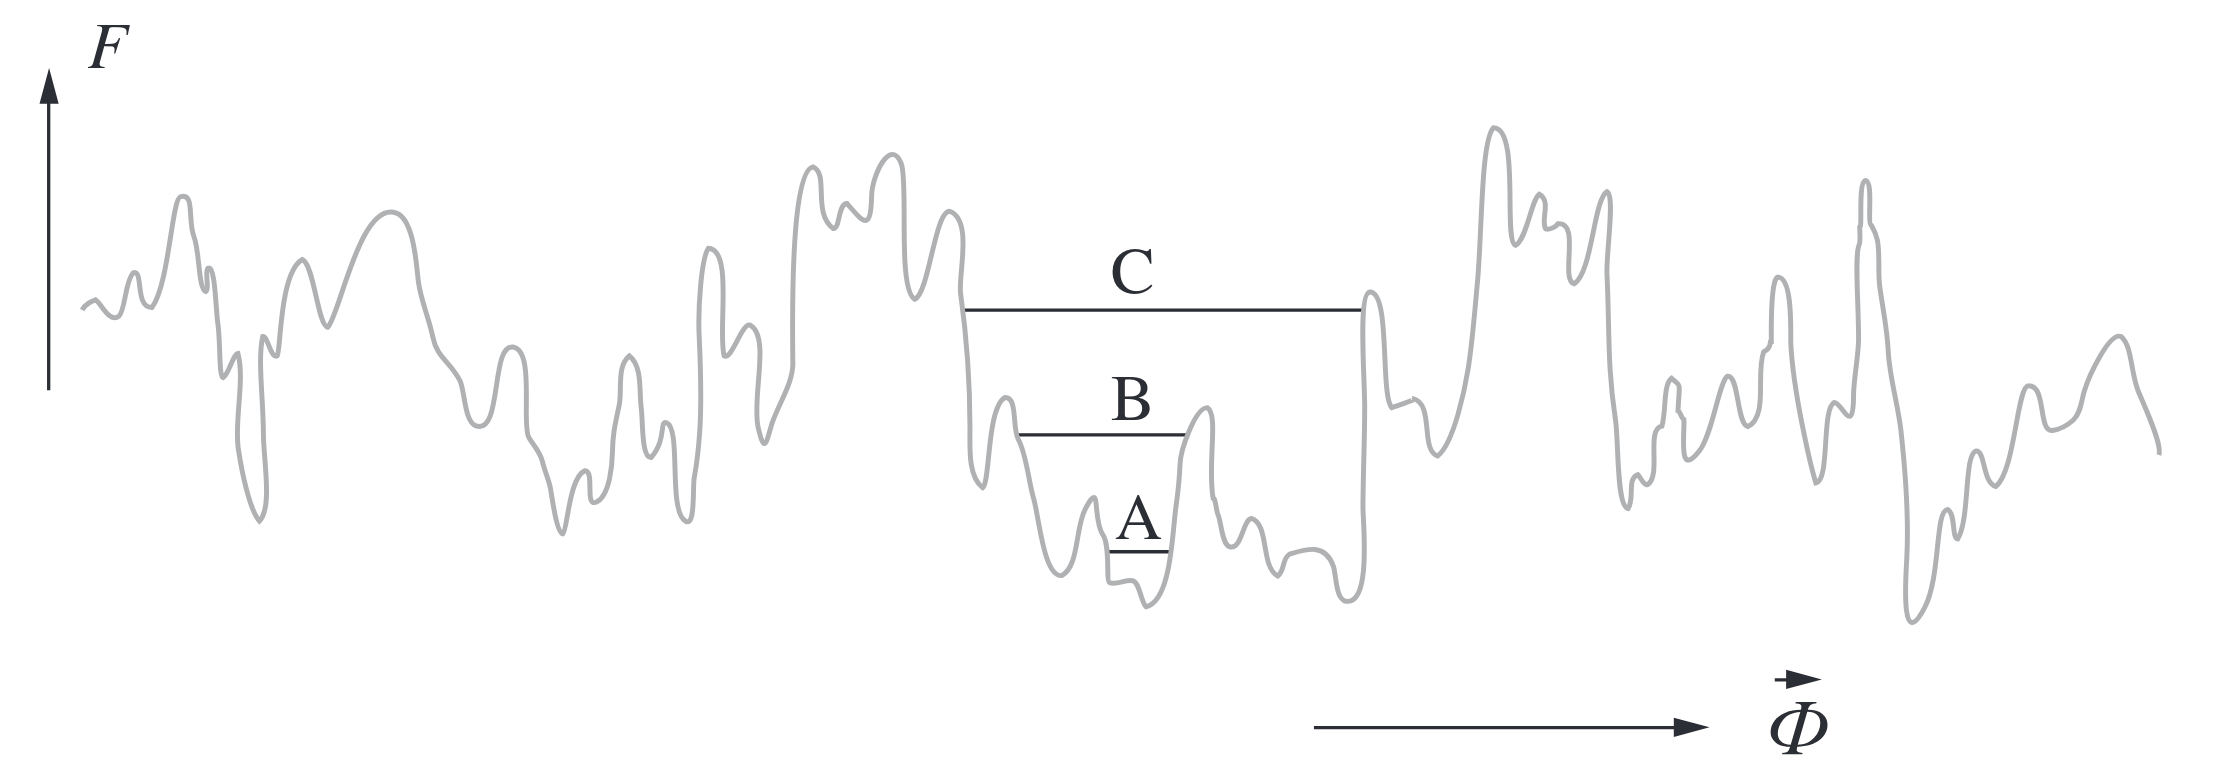
\includegraphics[width=0.8\textwidth]{Figures/spin-glass-rugged-energy-landscape.png}
    \caption[Un exemple de paysage énergétique d'un système de verre de spin.]{Un exemple de paysage énergétique d'un système de verre de spin en fonction des différentes configurations de spins possibles. Image tirée de~\protect\cite{stein2013spin}.}
    % Les multiples minimums locaux font en sorte que les algorithmes prennent du temps à résoudre le problème.
    \label{fig:spin-glass-rugged-energy-landscape}
\end{figure}
Cela fait en sorte que les algorithmes d'optimisation qui tentent de travailler sur ces modèles afin de trouver un état fondamental (ou la fonction de partition) d'un système ont tendance à être piégés dans ces minimums locaux, menant à des temps d'exécution exponentiellement longs.
On peut donc dire que les modèles de verre de spin sont simples à décrire, mais difficiles à résoudre.

% Les modèles pour les verres de spin sont, comme on le voit avec les $3$ modèles brièvement présentés, simple à décrire, mais ils sont toutefois difficiles à résoudre.
% Par résoudre, on entend ici de trouver un état fondamental du système ou d'évaluer sa fonction de partition.
% Une raison de cette difficulté vient du fait que ces modèles présentent des paysages énergétiques aillant une allure <<~accidentée~>>~\cite{stein2013spin}, piégeant les algorithmes d'optimisation dans des minimums locaux et conduisant à des temps d'exécution exponentiellement longs.
% Un exemple de paysage énergétique accidenté est présenté à la figure~\ref{fig:spin-glass-rugged-energy-landscape}.
% \begin{figure}[h]
%     \centering
%     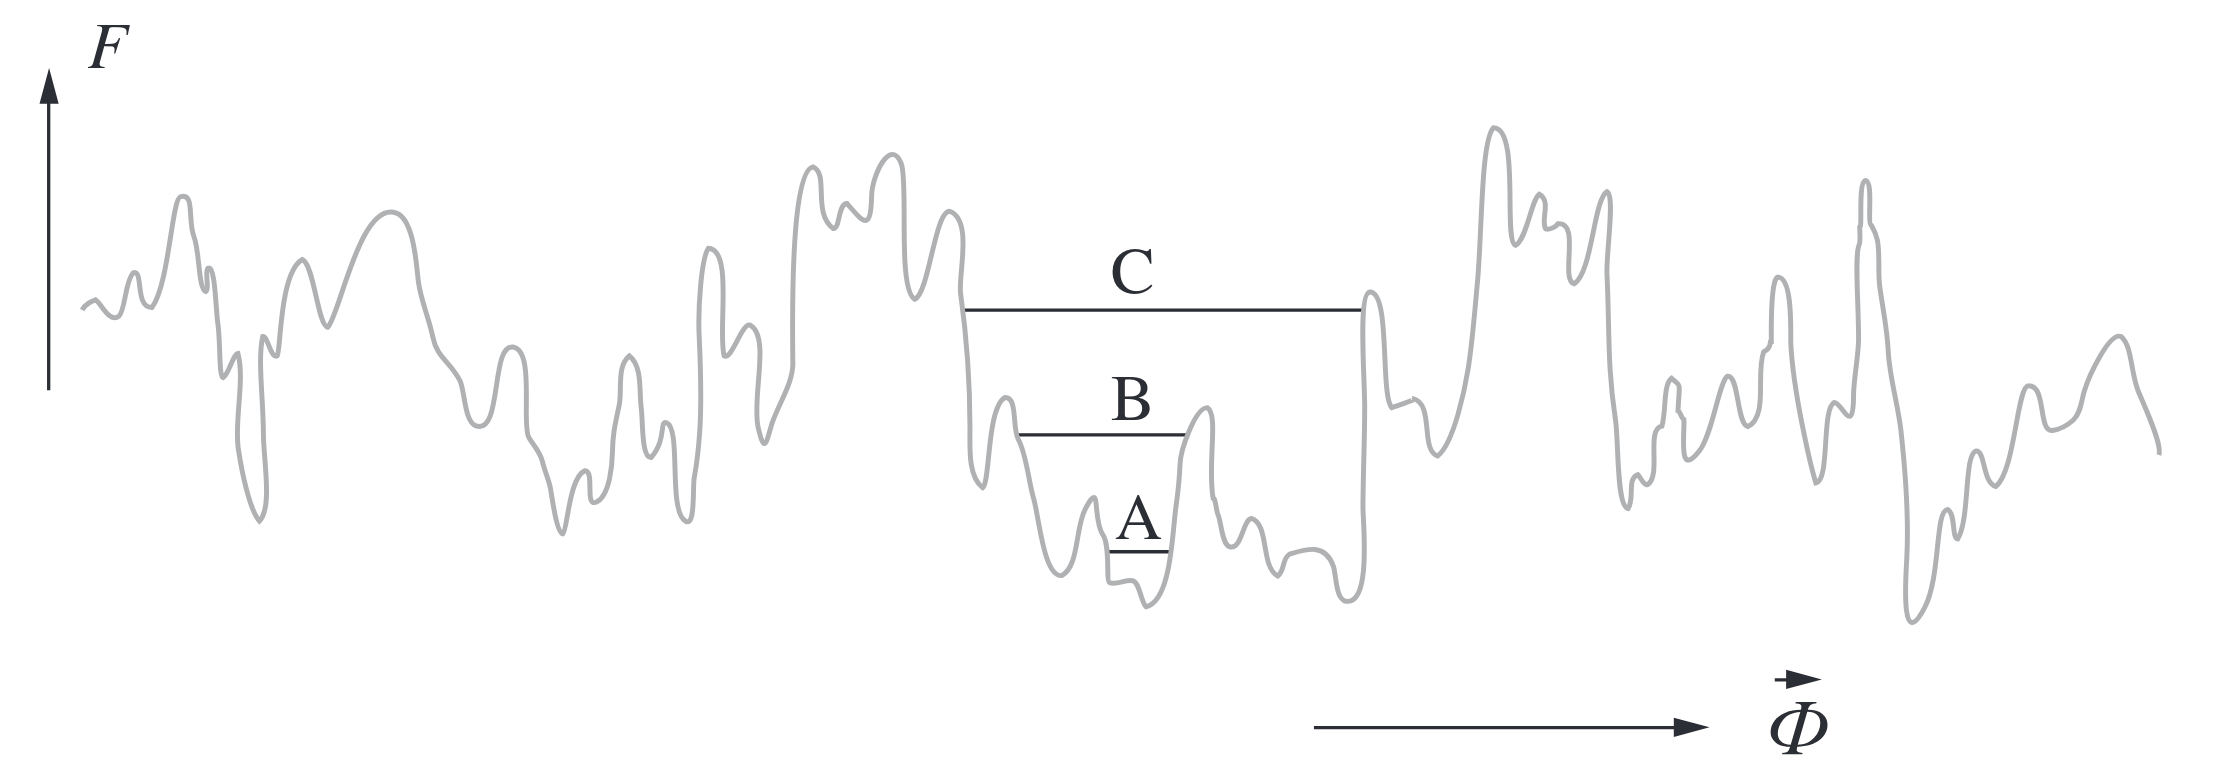
\includegraphics[width=0.9\textwidth]{Figures/spin-glass-rugged-energy-landscape.png}
%     \caption[Un exemple de paysage énergétique d'un système de verre de spin. Les multiples minimums locaux font en sorte que les algorithmes prennent du temps à résoudre le probléme. Image tirée de~\cite{}.]{Un exemple de paysage énergétique d'un système de verre de spin. Les multiples minimums locaux font en sorte que les algorithmes prennent du temps à résoudre le probléme. Image tirée de~\cite{stein2013spin}.}
%     \label{fig:spin-glass-rugged-energy-landscape}
% \end{figure}

Un contre-exemple connu de la difficulté de résolution d'un problème avec les verres de spin est le modèle $p$-spin, expliqué plus en profondeur dans la section~\ref{sec:p-spin} qui suit.
Ce modèle, quoique plus simple que les autres décrits dans cette section, possède lui aussi un paysage énergétique accidenté dans un certain régime de paramètres, mais sa résolution se fait tout de même facilement.

\section{Le modèle \texorpdfstring{$p$}{p}-spin} \label{sec:p-spin}
% Le modèle $p$-spin est une formulation aléatoire du modèle de Bethe dans lequel $p$ spins (des spins d'Ising) sont aléatoirement couplés~\cite{mezard_alternative_2002}.
Le modèle $p$-spin est une variante du modèle général des verres de spin dans lequel seulement les $p$ plus proches voisins (des spins d'Ising) interagissent ensemble.
Il peut en fait être vu par une formulation aléatoire du modèle de Bethe dans lequel $m$ couplages de $p$ spins sont aléatoirement définis dans un système contenant $n$ spins~\cite{mezard_alternative_2002}.
% de manière ferromagnétique ou antiferromagnétique.
De par sa simplicité et sa structure, un système $p$-spin se représente aisément de manière visuelle en utilisant un \emph{graphe}, terme défini à la définition~\ref{def:graph}.
\begin{definition}\label{def:graph}
    Un \textbf{graphe} $G = (V, E)$ correspond à un ensemble de sommets $V$ et d'arêtes $E$, où $E = \{uv\ |\ u, v \in V\}$. Afin de visualiser ce concept, un graphe possédant six sommets  et sept arêtes est représenté à la figure~\ref{fig:random-graph}.
\end{definition}
\begin{figure}[h]
    \centering
    \includegraphics[width=0.7\textwidth]{Figures/graph_example.pdf}
    \caption[Graphe contenant six sommets et sept arêtes.]{Graphe contenant six sommets $V = \{v_1, v_2, v_3, v_4, v_5, v_6\}$ et sept arêtes $E = \{v_1v_6, v_2v_3, v_2v_6, v_3v_4, v_3v_5, v_4v_5, v_5v_6\}$.}
    \label{fig:random-graph}
\end{figure}
En effet, ce modèle peut se modéliser par un graphe $G = (U, V, E)$ où $U$ correspond à l'ensemble de sommets qui représentent les $|U| = n$ spins, $V$ correspond à l'ensemble de sommets qui représentent les $|V| = m$ termes d'interaction et $E$ correspond à l'ensemble d'arêtes qui connectent les sommets de $U$ avec $V$.
La définition de l'ensemble $E$ fait en sorte que les sommets en $U$ ne se connectent qu'avec ceux qui se trouvent en $V$, et vice-versa, ce qui revient à dire qu'il est un graphe \emph{biparti}.
Un exemple de ce type de graphe est représenté à la figure~\ref{fig:bipartite-graph}.
\begin{figure}[h]
    \centering
    \includegraphics[width=0.55\textwidth]{Figures/bipartite-graph-example.pdf}
    \caption[Exemple de graphe biparti.]{Exemple de graphe biparti, où aucune arête ne connecte deux sommets de même type (carrés et cercles).}
    \label{fig:bipartite-graph}
\end{figure}
Cette représentation permet la définition suivante de l'hamiltonien pour ce modèle:
% Le modèle $p$-spin est entièrement défini par l'hamiltonien $\mathcal{H}$ suivant:
\begin{equation} \label{eq:ham_p-spin}
    \mathcal{H} = \frac{1}{2} \left[m -\sum_{v \in V} J_{v}\prod_{u \in N(v)} \sigma_{u} \right],
\end{equation}
où $J_v \in \left\{\pm1\right\}$ correspond au couplage des $p$ interactions au sommet $v$, $\sigma_u \in \left\{\pm1\right\}$ est le spin présent au sommet $u$ et $N(v) \subset U$ est l'ensemble des $p$ spins qui interagissent ensemble au sommet $v$.
Ce système contient donc des spins d'Ising qui interagissent de manière ferromagnétique ou antiferromagnétique avec la même intensité partout.
L'étude principale de cet hamiltonien dans ce projet revient à <<~simplement~>> \emph{compter} le nombre de configurations de spins $\sigma_u$ qui donnent une énergie nulle au système pour un ensemble donné de graphes.
En d'autres mots, cela revient à évaluer la \emph{fonction de partition} $Z$ à température nulle de ces systèmes.
L'équivalence entre ces deux problèmes est expliquée plus en détail à l'annexe~\ref{annexe:partition-fn-and-counting}.
% En effet, en partant de la définition générale de cette fonction, on peut écrire:
% \begin{equation}
%     \begin{split}
%         Z &= \sum_{j} e^{-\beta E_j}\\
%         &= N_{\text{fond}}e^{-\beta E_{\text{fond}}} + \cdots\text{, à cause de la dégénérescence}\\
%         &= N_{\text{fond}} + \cdots\text{, en posant $E_{\text{fond}} = 0$}\\
%         &= N_{\text{fond}}\text{, à température nulle}.
%     \end{split}
% \end{equation}
% Ici, la première égalité énumère toutes les configurations possibles du système physique avec $j$.
% Dans la seconde égalité, $N_{\text{fond}}$ correspond au nombre d'états fondamentaux, soit le nombre de configurations associées à l'énergie fondamentale $E_{\text{fond}}$ et les autres termes de la somme sont ceux qui sont associés aux configurations reliées à des énergies supérieures à $E_{\text{fond}}$.
% La troisième égalité utilise le fait qu'on peut poser $e^{-\beta E_{\text{fond}}} = 1$ puisqu'il est toujours possible de modifier la définition du système afin que son énergie fondamentale soit nulle.
% Finalement, en prenant la limite $T \rightarrow 0$, tous les termes dépendants de la température dans la somme deviennent nulles, nous laissant avec la quatrième égalité.
%------------------------

% La définition générale de cette fonction est la suivante:
% \begin{equation}\label{eq:partition-function1}
%     Z = \sum_{j} e^{-\beta E_j},
% \end{equation}
% où $\beta = \frac{1}{k_B T}$, $j$ énumère toutes les configurations possibles du système étudié, $k_B$ est la constante de Boltzmann et $T$ est la température.
% À cause de la dégénérescence retrouvée dans les verres de spin, principalement à cause du phénomène de frustration, l'équation~\ref{eq:partition-function1} peut s'écrire comme suit:
% \begin{equation}\label{eq:partition-function2}
%     Z = N_{\text{fond}}e^{-\beta E_{\text{fond}}} + \cdots,
% \end{equation}
% où $N_{\text{fond}}$ est le nombre d'états fondamentaux --- le nombre de configurations associées à l'énergie fondamentale $E_{\text{fond}}$ --- et les autres termes dans la somme correspondent aux configurations avec des énergies supérieures.
% Comme il est toujours possible de modifier la définition du système afin que son énergie fondamentale soit nulle, on se retrouve avec $e^{-\beta E_{\text{fond}}} = 1$, donc l'équation~\ref{eq:partition-function2} devient:
% % Comme il est toujours possible de modifier la définition du système afin que son énergie fondamentale soit nulle, on peut enlever la dépendance en température du premier terme de l'équation~\ref{eq:partition-function2}:
% \begin{equation}
%     Z = N_{\text{fond}} + \cdots.
% \end{equation}
% Finalement, lorsqu'on pose $T \rightarrow 0$, on a que $e^{-\beta E_j} \rightarrow 0$, ce qui fait en sorte quetous les termes dépendants de la température disparaissent, nous laissant avec:
% \begin{equation}
%     Z = N_{\text{fond}}.
% \end{equation}
%----------------------
% \begin{definition}\label{def:partition-function}
%     En mécanique statistique, la \textbf{fonction de partition} est une fonction qui décrit les propriétés statistiques d'un système dans son état d'équilibre thermodynamique. Elle est une fonction qui additionne tous les états possibles d'un système, fournissant une mesure du poids statistique de ces états.
% \end{definition}
% L'énergie totale d'un système de ce type de problème peut s'écrire comme suit:
% \begin{equation}\label{eq:p-spin_energy}
%     E(\vec{\sigma}) = \sum_{v \in V} E(\vec{\sigma}_{\{N(v)\}}),
% \end{equation}
% ce qui permet de définir la fonction de partition de la manière suivante:
% \begin{equation}\label{eq:p-spin_partition-fn}
%     Z = \sum_{\vec{\sigma}} e^{-\beta E(\vec{\sigma})} = \sum_{\vec{\sigma}} \prod_{v \in V}e^{-\beta E(\vec{\sigma}_{\{N(v)\}})}.
% \end{equation}
% Cette expression sera utile plus tard dans la définition de ce problème en réseau de tenseurs.

À toute fin pratique, il est possible de réécrire l'hamiltonien de l'équation~\ref{eq:ham_p-spin} en définissant les termes de couplage et de spins d'une autre manière.
Comme les valeurs que les spins peuvent prendre se trouvent dans l'ensemble $\{\pm 1\}$, on peut introduire des variables \emph{booléennes} --- $b_v$ et $x_u$ ---, de la manière suivante:
\begin{equation}\label{eq:new_ham_p-spin1}
    \mathcal{H} = \frac{1}{2} \left[m -\sum_{v \in V} (-1)^{b_v}\prod_{u \in N(v)} (-1)^{x_u} \right] = \frac{1}{2} \left[m -\sum_{v \in V} (-1)^{b_v + \sum_{u \in N(v)} x_u} \right],
\end{equation}
où les termes de couplage et les spins sont redéfinis comme étant respectivement $J_v = (-1)^{b_v}$ et $x_u = (-1)^{x_u}$.
Ce changement de variable correspond simplement à faire la conversion entre les valeurs $\pm 1$ et l'ensemble $\{0, 1\}$.
Comme ces nouvelles variables sont booléennes, on ne s'intéresse qu'à la parité de l'exposant de $-1$, ce qui nous permet de finalement définir cet hamiltonien comme suit:
\begin{equation} \label{eq:new_ham_p-spin2}
    \mathcal{H} = \frac{1}{2} \left[m -\sum_{v \in V} (-1)^{b_v + \sum_{u \in N(v)} x_u\mod{2}} \right].
\end{equation}
Avec cette nouvelle expression de $\mathcal{H}$, trouver une des configuration de spins $\vec{\sigma}$ qui mène à l'énergie minimale du système revient à résoudre l'équation suivante:
\begin{equation}
    \begin{split}
        b_v + \sum_{u \in N(v)} x_u = 0 &\mod{2}\ \forall\ v \in V,\\
        \implies b_v = \sum_{u \in N(v)} x_u &\mod{2}\ \forall\ v \in V.
    \end{split}
\end{equation}
Cette nouvelle expression à résoudre peut directement se traduire comme le système d'équations linéaires suivant:
\begin{equation} \label{eq:Bx=b}
    B\vec{x} = \vec{b} \mod 2,
\end{equation}
où $B \in \{0, 1\}^{m \times n}$ est la \emph{matrice de biadjacence} du graphe biparti $G$ qui modélise le problème initial, $\vec{x} \in \left\{ 0,1 \right\}^n$ encode la configuration des $n$ spins et $\vec{b} \in \left\{ 0,1 \right\}^m$ encode les $m$ couplages.
Les éléments de la matrice de biadjacence se définissent comme suit:
\begin{equation}\label{eq:biadjacency-matrix}
    B_{vu} = 
    \begin{cases}
            1, & \text{si $u \in N(v)$,}\\
            0, & \text{sinon.}
    \end{cases}
\end{equation}
On a donc que si un spin $\sigma_u$ interagit avec ceux qui sont dans $N(v)$ (que $B_{vu} = 1$) une arête se trouve entre le terme d'interaction $v$ et ce même spin dans $G$.

Déterminer les configurations de spins qui minimisent l'énergie de ce type de système revient à résoudre l'équation matricielle~\ref{eq:Bx=b} et compter le nombre de ces configurations revient à faire d'autres manipulations sur cette même expression.
Ces autres manipulations correspondent à convertir ce problème sous la forme de problème de \emph{satisfiabilité booléenne} (SAT), plus précisément le \#$p$-XORSAT dans le cas du modèle $p$-spin.
Ces termes sont définis dans le chapitre~\ref{ch:SAT}.



\chapter{Satisfiabilité booléenne} \label{ch:SAT}
% \lettrine{U}{n} problème d'optimisation tel que l'optimisation de horaires pour les envols et les attrissages d'avions, le problème sac-à-dos ou même le problème du voyageur de commerce sont des problèmes d'optimisation utilisés dans la vie de tous les jours.
% Ces problèmes ont tous une similarité, il est possible de les résoudre en utilisant le concept de la satisfiabilité booléenne, mais ils sont difficiles à résoudre.
% C'est pourquoi 

\section{Définition}\label{sec:def-SAT}
Dans sa forme la plus générale, un problème SAT consiste à déterminer si une formule logique, construite à l'aide d'un ensemble de variables booléennes $\vec{x} = (x_1, x_2, ..., x_n)$ et des opérateurs de conjonction ($\wedge$), de disjonction ($\vee$) et de négation ($\neg$), peut être rendue vraie, c'est-à-dire, si elle est \textit{satisfiable}~\cite{garey1979computers}.
Le problème SAT se caractérise toujours par une conjonction de \emph{clauses} qui sont elles-mêmes des disjonctions de variables sur lesquelles l'opération de négation peut être appliquée.

% Afin de mieux visualiser ce type de problème, voici un exemple aléatoire avec $n = 4$ variables et $m = 2$ clauses:
Afin de mieux visualiser et comprendre ce type de problème, un exemple aléatoire avec $n = 4$ variables et $m = 2$ clauses est donné à l'équation~\ref{eq:SAT-example}.
\begin{equation}\label{eq:SAT-example}
    \phi(\vec{x}) = (x_0 \vee \neg x_2 \vee x_3) \wedge (x_1 \vee x_2).
\end{equation}
Essayons maintenant de déterminer une solution qui satisfait ce problème.
Cela peut se faire en utilisant une approche exhaustive où on regarde chacune des combinaisons possibles pour ces clauses.
Pour la clause $c_0 = x_0 \vee \neg x_2 \vee x_3$, cette analyse est faite dans le tableau~\ref{table:c1} et la même est faite pour $c_1 = x_1 \vee x_2$ dans le tableau~\ref{table:c2}.
% \begin{table}[h]
%     \centering
%     \begin{tabular}{|c c c||c|}
%         \hline
%         $x_1$ & $x_3$ & $x_4$ & $x_1 \vee x_3 \vee x_4$ \\
%         \hline
%         0 & 0 & 0 & 0 \\
%         \hline
%         0 & 0 & 1 & 1 \\
%         \hline
%         0 & 1 & 0 & 1 \\
%         \hline
%         0 & 1 & 1 & 1 \\
%         \hline
%         1 & 0 & 0 & 1 \\
%         \hline
%         1 & 0 & 1 & 1 \\
%         \hline
%         1 & 1 & 0 & 1 \\
%         \hline
%         1 & 1 & 1 & 1 \\
%         \hline
%     \end{tabular}
%     \caption{Toutes les combinaisons de variables possibles pour la clause $c_1$.}
%     \label{table:c1}
% \end{table}
% \begin{table}[h]
%     \centering
%     \begin{tabular}{|c c||c|}
%         \hline
%         $x_2$ & $x_3$ & $x_2 \vee x_3$ \\
%         \hline
%         0 & 0 & 0\\
%         \hline
%         0 & 1 & 1\\
%         \hline
%         1 & 0 & 1\\
%         \hline
%         1 & 1 & 1\\
%         \hline
%     \end{tabular}
%     \caption{Toutes les combinaisons de variables possibles pour la clause $c_2$.}
%     \label{table:c2}
% \end{table}
\begin{table}[h]
    \parbox{.48\linewidth}{
        \centering
        \begin{tabular}{|c c c c||c|}
            \hline
            $x_0$ & $x_2$ & $\neg x_2$ & $x_3$ & $x_0 \vee \neg x_2 \vee x_3$ \\
            \hline
            0 & 0 & 1 & 0 & 1 \\
            \hline
            0 & 0 & 1 & 1 & 1 \\
            \hline
            0 & 1 & 0 & 0 & 0 \\
            \hline
            0 & 1 & 0 & 1 & 1 \\
            \hline
            1 & 0 & 1 & 0 & 1 \\
            \hline
            1 & 0 & 1 & 1 & 1 \\
            \hline
            1 & 1 & 0 & 0 & 1 \\
            \hline
            1 & 1 & 0 & 1 & 1 \\
            \hline
        \end{tabular}
        \caption{Toutes les combinaisons de variables possibles pour la clause $c_0$.}
        \label{table:c1}
    }
    \hfill
    % \hspace{0.001\textwidth}
    \parbox{.48\linewidth}{
        \centering
        \begin{tabular}{|c c||c|}
            \hline
            $x_1$ & $x_2$ & $x_1 \vee x_2$ \\
            \hline
            0 & 0 & 0\\
            \hline
            0 & 1 & 1\\
            \hline
            1 & 0 & 1\\
            \hline
            1 & 1 & 1\\
            \hline
        \end{tabular}
        \caption{Toutes les combinaisons de variables possibles pour la clause $c_1$.}
        \label{table:c2}
    }
\end{table}
Une solution pour $\phi(\vec{x})$ en est une pour laquelle $c_0$ et $c_1$ sont satisfaites en même temps.
Avec ces deux énumérations de toutes les possibilités de configurations des variables dans les clauses, il est facile de voir que la configuration $\vec{x} = (0, 1, 0, 0)$ en est une qui satisfait les deux clauses en même temps, donc le problème.
L'utilisation de cette méthode est simple dans ce cas puisque $n$ est petit, mais lorsque le nombre de variables augmente, elle devient impossible à utiliser.
En effet, si $\phi(\vec{x})$ contient $n$ variables alors il y a $2^n$ configurations possibles pour les variables.
Cela signifie que pour un grand $n$, il devient impossible de faire ce type de recherche exhaustive.

Le problème SAT a été le premier problème démontré comme appartenant à la classe de complexité \textbf{NP-complète} par Stephen Cook~\cite{cook1971}.
% --------- Début du nouvellement ajouté -----------------
Avant de définir cette classe de complexité, il est important de comprendre que les problèmes se séparent, d'après les connaissances d'aujourd'hui~\cite{millenniumPrizeProblems}, en deux; les problèmes dits \emph{faciles} (\textbf{P}) et ceux qui sont \emph{difficiles} (\textbf{NP}).
Ceux qui sont facilement solubles sont ceux qui sont dans la classe \textbf{P}, soient tous les problèmes de décision qui sont solubles dans un temps polynomial.
Ceux qui sont difficiles se retrouvent dans la classe \textbf{NP} (\textit{nondeterministic polynomial time} en anglais), donc tous les problèmes de décision pour lesquels la solution peut se faire vérifier facilement (dans un temps polynomial).
Avec cela, on peut maintenant définir la classe \textbf{NP-complète} comme suit:
% --------- Fin du nouvellement ajouté -------------------
% Cette classe de complexité contient deux points importants: elle regroupe des problèmes qui font parties de la classe de complexité \emph{NP} et elle est \emph{complète}.
% Les définitions de ces deux classes de complexité se retrouvent respectivement aux définitions~\ref{def:NP} et~\ref{def:NP-complete}.
% Pour ces deux catégories, tout problème qui s'y trouve est un problème pour lequel il est facile de vérifier si une solution est bonne, mais difficile de trouver cette dite solution.
% La hiérarchie de ces classes de complexité est montrée dans la figure~\ref{fig:complexites}, où on voit aussi les classes \emph{P} et \emph{NP-difficile} , toutes deux définies respectivement aux définitions~\ref{def:P} et~\ref{def:NP-hard}.
% \begin{definition}\label{def:P}
%     La classe de complexité \textbf{P} contient tous les problèmes de décision qui sont solvables facilement (dans un temps polynomial).
% \end{definition}
% \begin{definition}\label{def:NP}
%     La classe de complexité \textbf{NP} (<<~nondeterministic polynomial time~>> en anglais) contient tous les problèmes de décision pour lesquels la solution peut se faire vérifier rapidement (dans un temps polynomial).
% \end{definition}
\begin{definition}\label{def:NP-complete}
    % La classe de complexité \textbf{NP-complet} est une classe qui englobe tous les problèmes $A$ dans NP pour lesquels il est possible de réduire tout autre problème NP $B$ à $A$ facilement (en temps polynomial).
    La classe de complexité \textbf{NP-complète} est une classe des problèmes \textbf{NP} auxquels tous les autres problèmes dans \textbf{NP} peuvent être réduits en temps polynomial.
\end{definition}
On retrouve ensuite la classe de complexité \textbf{\#P}, qui rassemble les problèmes qui ont comme objectif de \emph{compter} le nombre de solution(s) de problèmes dans \textbf{NP}.
Il y a aussi la classe \textbf{\#P-complète}, qui englobe tous les problèmes se retrouvant dans \textbf{\#P} vers lesquels il est possible de réduire tout autre problème de cette classe facilement (en temps polynomial).
Les problèmes qui s'y retrouvent sont tous au moins aussi difficiles que ceux qui sont dans la classe \textbf{NP-complète}.
% \begin{definition}\label{def:NP-hard}
%     La classe de complexité \textbf{NP-difficile} contient les problèmes qui sont au moins aussi difficiles que ceux se trouvant dans la classe NP-complet, sans toutefois se limiter aux problèmes de décision.
% \end{definition}
Finalement, dans la hiérarchie des classes de complexité montrée à la figure~\ref{fig:complexites}, on retrouve la classe \textbf{NP-difficile}. 
Celle-ci englobe tous les problèmes qui sont au moins aussi difficiles que ceux se trouvant dans la classe \textbf{NP-complète}, sans toutefois se limiter aux problèmes de décision.
\begin{figure}[h]
    \centering
    % ajouter figure de la hiérarchie des classes de complexités de P à NP-difficile
    \includegraphics[width=0.6\textwidth]{Figures/complexity_classes_hierarchy.pdf}
    \caption[Schéma de la hiérarchie des classes de complexité.]{Schéma de la hiérarchie des classes de complexité (en supposant que P~$\ne$~NP).}
    \label{fig:complexites}
\end{figure}

% Les deux autres classes de complexités qui n'ont pas été définies plus haut, mais qui se trouvent dans la figure~\ref{fig:complexites}, sont \emph{\#P} et \emph{\#P-complet}, définies respectivement aux définitions~\ref{def:sharp-P} et~\ref{def:sharp-P-complete} ci-dessous.
% Celles-ci englobent les problèmes pour lesquels l'objectif est de compter le nombre de solution satisfaisant le problème initial.
% Un exemple de problème de ce type est \#SAT, le problème pour lequel l'objectif est de déterminer le nombre de configurations de variables qui satisfont un problème donné.
% \begin{definition}\label{def:sharp-P}
%     La classe de complexité \textbf{\#P} comprend les problèmes de comptage liés aux problèmes de décision présents dans NP.
%     Plus précisément, un problème appartient à \#P s'il consiste à compter le nombre de solutions qui satisfont un problème donné de la classe NP.
% \end{definition}
% \begin{definition}\label{def:sharp-P-complete}
%     La classe de complexité \textbf{\#P-complet} est une classe qui englobe tous les problèmes $A$ dans \#P pour lesquels il est possible de réduire tout autre problème \#P $B$ à $A$ facilement (en temps polynomial).
%     Les problèmes dans \#P-complet sont au moins aussi difficiles que ceux se trouvant dans NP-complet.
% \end{definition}


% Ces types de problèmes ne sont pas seulement des problèmes purement théoriques, puisqu'ils peuvent être utillisés dans notre vie de tous les jours.
% Certains exmples concrets sont le \emph{problème de voyageur de commerce} et le \emph{problème du sac à dos}.
% Le premier est un problème dans lequel un voyageur de commerce souhaite trouver un chemin qui va le faire passer par les $N$ villes (destinations) dans lesquelles il doit y faire une livraison sans y repasser par la suite tout en minimisant le coût (la distance parcourue) de ce voyage.
% Ce problème se retrouve par exemple dans l'optimisation des chemins pour les camionneurs ou pour les livreurs.
% Le second est un problème dans lequel, par exemple, une personne souhaite partir en randonnée et veut optimiser sons sac à dos au niveau de la nourriture.
% Elle souhaite minimiser le poids de cette nourriture tout en maximisant ses apports nutritifs.

En ajoutant une contrainte stipulant que chacune des clauses d'un problème SAT possède exactement $k$ variables, on se retrouve à étudier le problème $k$-SAT qui est, lui aussi, dans la catégorie de complexité \textbf{NP-complète}.
Compter le nombre de solution(s) satisfaisant ce type de problème correspond au problème \#$k$-SAT et lui aussi se retrouve dans la catégorie de complexité \textbf{\#P-complète}, pour toutes les valeurs de $k \geq 2$~\cite{valiant_complexity_1979}.

Le problème $k$-SAT possède plusieurs variantes, comme \textit{$1$-in-$3$} SAT et \textit{not-all-equal} 3-SAT (NAE3-SAT), et la plupart se retrouvent dans la même classe de complexité que celui-ci.
De plus, chacune d'elle peut se caractériser par le paramètre $\alpha \equiv m / n$, la densité de clauses.
Ce paramètre est relié au phénomène de transition de phase dans ces problèmes.
Pour le problème de type $k$-SAT, ce phénomène se produit à une certaine valeur du paramètre $\alpha$ où la probabilité que le problème soit soluble passe drastiquement de $1$ vers $0$.
Dans le cas du problème $k$-SAT avec $k = 3$, la transition est montrée dans la figure~\ref{fig:SAT_phase-transition}.
\begin{figure}[h]
    \centering
    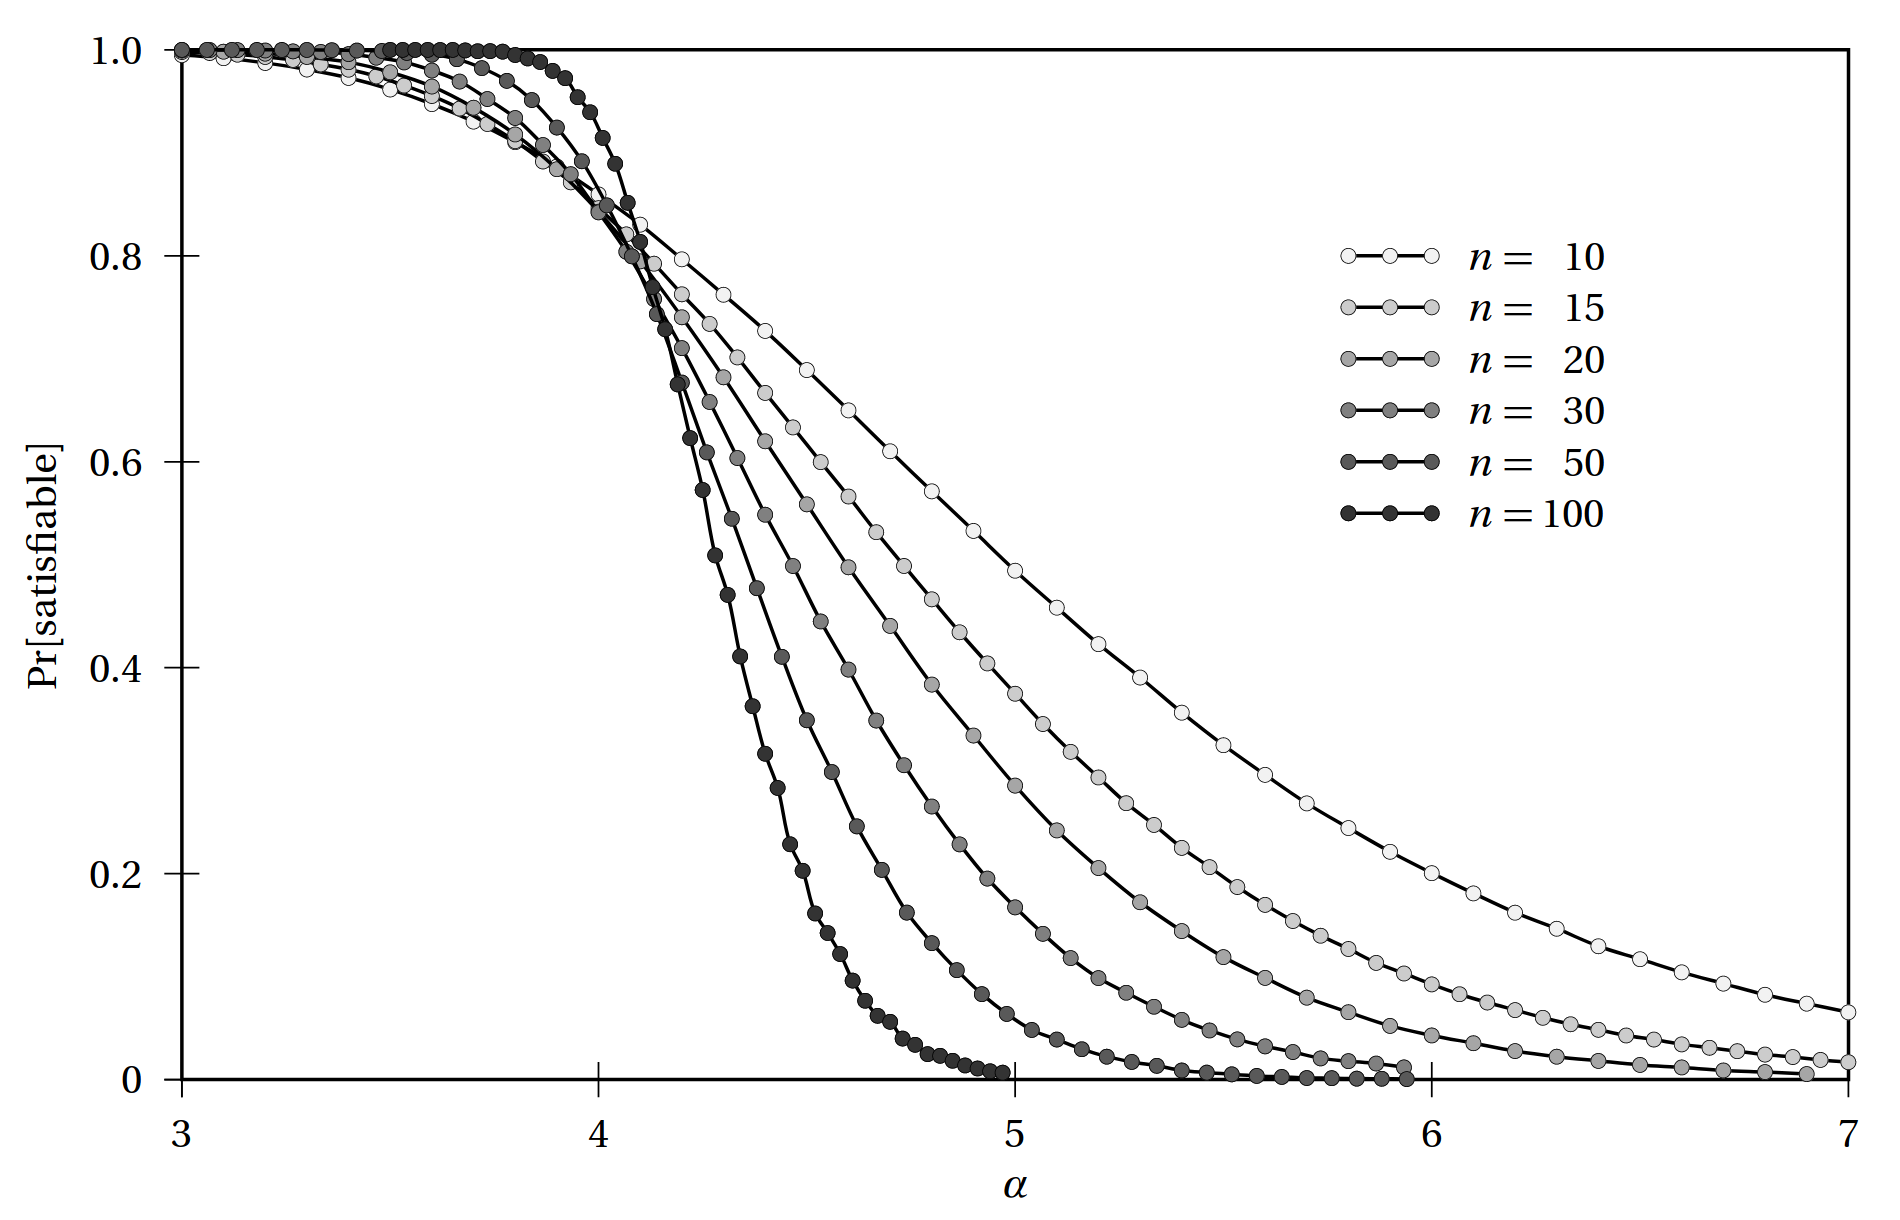
\includegraphics[width=0.7\textwidth]{Figures/SAT_phase-transition.png}
    \caption[La probabilité de satisfaction d'un problème $3$-SAT en fonction de la densité de clauses $\alpha$.]{La probabilité de satisfaction d'un problème $3$-SAT en fonction de la densité de clauses $\alpha$. On voit que plus le nombre de variables $n$ augmente, plus la chute devient abrupte. En fait, si on traçait la courbe dans la limite thermodynamique ($n \rightarrow \infty$), il y aurait un passage instantané de 1 vers 0 à $\alpha = \alpha_c$. Image tirée de \emph{The Nature of Computation}~\protect\cite{moore_nature_2011}.}
    \label{fig:SAT_phase-transition}
\end{figure}
Comme on peut le voir dans cette figure, le problème $3$-SAT passe de \textit{satisfiable} à \textit{non-satisfiable} à $\alpha \approx 4.267$~\cite{moore_nature_2011}.
On appelle cette transition: la transition de phase SAT-UNSAT.

Maintenant que la notion de problème SAT est définie, on peut s'attaquer au problème qui modélise le modèle de $p$-spin définit à l'équation~\ref{eq:Bx=b}.
Ce problème est, comme mentionné à la fin de la section~\ref{sec:p-spin}, $p$-XORSAT, qui est défini dans la section~\ref{sec:k-xorsat}.


\section{Le problème \#\texorpdfstring{$k$}{k}-XORSAT}\label{sec:k-xorsat}
Le problème $k$-XORSAT est le problème principal dans ce mémoire dans le cadre de l'analyse du problème $p$-spin.
Afin de relier les deux, il suffit de poser $k = p$ et de respecter les encodages mentionnés après l'équation~\ref{eq:Bx=b}, et la conversion est faite.
La présentation du problème général dans cette section est faite en utilisant seulement $k$, la variable $p$ sera utilisée plus tard dans le chapitre~\ref{ch:tns-and-p-xorsat}.

Ce problème ne requiert qu'une seule modification des opérateurs dans les clauses par rapport au problème standard $k$-SAT.
L'opérateur de disjonction y est remplacé par l'opérateur de sommation modulo $2$ ($\oplus$), qui se fera nommer <<~sommation booléenne~>> au travers de ce mémoire puisque les variables qui se retrouvent dans les problèmes analysés sont booléennes.
Avec la matrice de biadjacence $B$ et le vecteur $\vec{b}$ de l'équation~\ref{eq:Bx=b}, on peut définir une instance $\phi(\vec{x})$ du problème $k$-XORSAT de la manière suivante:
\begin{equation}\label{eq:xorsat_def}
    \begin{split}
        \phi(\vec{x}) &= \bigwedge_{v = 0}^{m - 1} c_v \text{, où }m = \alpha n,\\
        c_v &= 1 \oplus b_v \oplus B_v \cdot \vec{x},\\
        \vec{x} &= \left(x_1, x_2, \ldots, x_n \right) \in \{0, 1\}^n,
    \end{split}
\end{equation}
où $B_v \in \{0, 1\}^n$ est la rangée $v$ de la matrice $B$, $b_v$ indique l'élément $v$ du vecteur $\vec{b}$ et $B_v \cdot \vec{x}$ indique la sommation booléenne des variables présentes dans la clause $c_v$.
Les éléments de $\vec{b}$ peuvent aussi être vus comme étant les parités requises pour satisfaire chacune des clauses du problème.
Lorsque $c_v = 1$, ce qui se produit lorsque $b_v \oplus B_v \cdot \vec{x} = 0$, on dit que la clause est \emph{satisfaite}.

Comme mentionné dans la section~\ref{sec:def-SAT}, lorsqu'on génère ces types d'instances de manière complètement aléatoire, on a que le paramètre de densité de clause $\alpha$ caractérise en grande partie le problème.
Pour le problème $k$-XORSAT en particulier, celui-ci contient deux transitions de phases~\cite{mezard_alternative_2002}.
La première se produit à $\alpha_d$, qui indique une transition \emph{dynamique} dans la structure de l'espace des solutions de manière à séparer (en distance de Hamming) les solutions en plusieurs \emph{grappes}.
La seconde se produit à la transition critique $\alpha_c$ où, avec une probabilité élevée, une instance devient non-satisfiable.
Celle-ci est conceptuellement équivalente à la transition de phase SAT/UNSAT montrée dans la figure~\ref{fig:SAT_phase-transition}.
Ce point montre une transition de phase similaire même lorsque $\vec{b} = \vec{0}$, ce qui signifie que $\vec{x} = \vec{0}$ est toujours une solution possible~\cite{ricci2001simplest}.
Afin de mieux comprendre les effets qu'a ce paramètre sur l'espace des solutions mentionnées pour $\alpha_d$, son évolution en fonction de $\alpha$ est schématisée à la figure~\ref{fig:solution-space}.
\begin{figure}[h]
    \centering
    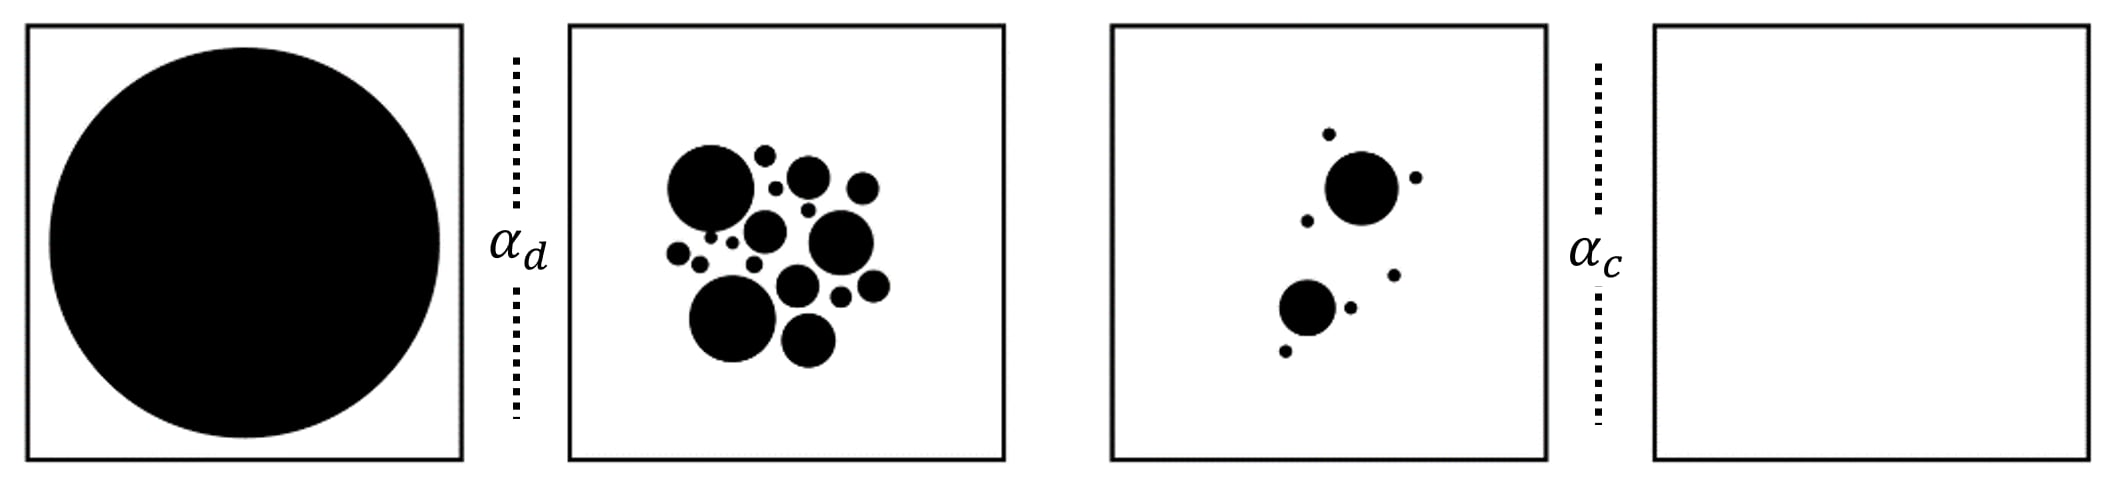
\includegraphics[width=0.77\textwidth]{Figures/solution_space_evolution.jpeg}
    \caption[L'évolution de l'espace des solutions pour le problème \mbox{$k$-XORSAT}.]{Schéma de l'évolution de l'espace des solutions pour le problème \mbox{$k$-XORSAT}. Image tirée de~\protect\cite{moore_nature_2011}.}
    \label{fig:solution-space}
\end{figure}
Dans le cas de $3$-XORSAT, ces deux paramètres sont $\alpha_d \approx 0.818$ et $\alpha_c \approx 0.918$~\cite{mezard_alternative_2002}.
De plus, comparativement aux autres variantes du problème \#$k$-SAT, le problème \#$k$-XORSAT ne se retrouve pas dans la classe de complexité \textbf{\#P-complète}, mais bien dans \textbf{P}, donc on sait qu'il est facile de le résoudre.
Ce point sera plus développé dans la section~\ref{subsec:GE}.

De nombreux algorithmes ont été adaptés afin d'être applicables sur le problème $k$-XORSAT, tels que le recuit quantique adiabatique~\cite{patil_obstacles_2019}, l'élimination gaussienne~\cite{braunstein_complexity_2002} et l'algorithme d'élimination de feuilles~\cite{mezard_alternative_2002} pour en nommer quelques-uns.
% un algorithme adiabatique quantique~\cite{farhi2000quantum}.
Dans les prochaines sections, on va commencer par définir l'algorithme utilisant l'élimination gaussienne (section~\ref{subsec:GE}) pour ensuite définir celui d'élimination de feuilles, une méthode graphique qui élimine la redondance dans le problème (section~\ref{subsec:leaf-removal-algorithm}) et on finit par définir une méthode graphique connue pour simplifier un problème donné (section~\ref{subsec:XORSAT-simplifications}).

% DON'T USE THIS
% Ce n'est pas par hasard que ce même $p$ se retrouve dans le nom de ces deux problèmes, car cette variable correspond directement à la même valeur dans les deux cas.
% En effet, avoir $p$ spins qui interagissent ensemble revient à avoir $p$ variables dans chacune des clauses du problème de satisfiabilité.

\subsection{Élimination gaussienne}\label{subsec:GE}
Étant donnée une instance $\phi(\vec{x})$ du problème $k$-XORSAT contenant $m$ clauses et $n$ variables, on commence par la traduire sous la forme de la matrice de biadjacence $B$ de l'équation~\ref{eq:Bx=b}.
Il est aussi nécessaire d'avoir les parités de chacune des clauses afin de pouvoir utiliser $\vec{b}$.
Par la suite, on applique l'élimination gaussienne sur la matrice augmentée $[B|\vec{b}]$, où toutes les opérations sont modulo deux.
Une fois cette étape terminée, si on retrouve au moins une incohérence dans le système, il n'existe aucune solution pouvant satisfaire ce problème.
Cette incohérence vient du fait qu'une ligne aurait la forme $[0\ 0\ \dots 0 | 1]$, ce qui n'a aucun sens puisque la somme modulo $2$ de plusieurs variables ayant un poids nul ne peut jamais être égale à un.
Toutefois, si ces incohérences ne sont pas présentes, alors le nombre de solutions satisfaisant le problème donné est:
\begin{equation}\label{eq:nb_sols_ge}
    \text{\#Solutions} = 2^{n - \mathrm{rang}(B)}.
\end{equation}

Dans~\cite{braunstein_complexity_2002}, les auteurs ont étudié les complexités en temps et en mémoire de l'élimination gaussienne pour la résolution du problème \#$k$-XORSAT avec $k = 3$ en utilisant une version de cet algorithme qu'ils définissent comme étant <<~simple~>>.
Cette version résout les équations linéaires présentes dans l'équation~\ref{eq:Bx=b} dans l'ordre dans lequel elles apparaissent déjà.
Ils y montrent que cet algorithme simple résout le problème donné avec une complexité en temps et en mémoire proportionnelle à $n$ pour $\alpha \leq 2/3$.
Lorsque ce paramètre dépasse le seuil de $2/3$, les complexités en temps et en mémoire deviennent respectivement $\propto n^3$ et $\propto n^2$.
Les auteurs ont également présenté une version <<~intelligente~>> de cet algorithme, dans laquelle les variables qui apparaissent dans le moins d'équations sont abordées en premier (en cas d'égalité, elles sont choisies arbitrairement).
On résout ensuite pour cette variable et on la substitue dans les équations restantes.
Ils font valoir que cette version plus intelligente résout le problème avec des ressources (le temps et la mémoire) proportionnelles à $n$ lorsque $\alpha < \alpha_d$.
Lorsque $\alpha > \alpha_d$, ces ressources passent respectivement à $\propto n^3$ et $\propto n^2$.

Ces changements de complexité pour ces deux versions de l'algorithme sont dus au fait que chaque étape de l'élimination gaussienne peut introduire de nouveaux $1$s dans $B$, augmentant ainsi leur densité en fonction du nombre d'éléments dans cette matrice.
Cette augmentation est suffisante pour modifier ces complexités, car la matrice ne reste pas creuse comme on peut le voir avec l'exemple donné dans la figure~\ref{fig:GE-ones-density}.
\begin{figure}[h]
    \centering
    \includegraphics[width=0.9\textwidth]{Figures/matrice.pdf}
    \caption[Évolution de la densité de $1$ lors de l'élimination gaussienne.]{Évolution de la densité de 1 lors de l'élimination gaussienne avec $n = m = 1024$ ($\alpha = 1$). Les points noir et blanc correspondent respectivement aux 0 et aux 1 dans la matrice et $t$ représente le pourcentage de complétion de l'algorithme. Image tirée de~\protect\cite{braunstein_complexity_2002}.}
    \label{fig:GE-ones-density}
\end{figure}


Lorsqu'on résout une équation qui contient une variable qui n'apparaît que dans celle-ci, on peut interpréter graphiquement le processus comme un algorithme d'\emph{élimination de feuilles}, décrit dans la section~\ref{subsec:leaf-removal-algorithm} suivante.
Cet algorithme donne une intuition quant à la raison pour laquelle la version <<~intelligente~>> de l'élimination gaussienne est plus efficace et aidera à expliquer le comportement de l'algorithme développé dans le cadre de ce projet qui utilise les réseaux de tenseurs.
Cet algorithme est expliqué plus tard dans les sections~\ref{sec:eliminate-redundancy-with-bond-compression} et~\ref{sec:sweeping-method}.

\subsection{Algorithme d'élimination de feuilles}\label{subsec:leaf-removal-algorithm}
Supposons qu'on a une instance $k$-XORSAT avec $k = 3$ et qu'une variable, que l'on définit comme étant $x_0$, n'apparaît que dans l'équation linéaire:
\begin{equation}\label{eq:c0-example}
    x_0 \oplus x_1 \oplus x_2 = b_0,
\end{equation}
qui correspond à la clause $c_0$ dans le problème.
Peu importe les valeurs que les variables $x_1$ et $x_2$ prennent, il est toujours possible de choisir $x_0$ de manière à satisfaire cette clause en la fixant à:
\begin{equation}\label{eq:x0-value}
    x_0 = x_1 \oplus x_2 \oplus b_0.
\end{equation}
En sachant cela, on peut enlever cette clause du problème initial, le résoudre, et définir la valeur de $x_0$ en fonction des deux autres variables à la fin.
% On a donc que satisfaire l'équation~\ref{eq:x0-value} permet de donner une configuration de variables qui satisfait le problème donné si et seulement si le problème simpifié est satisfiable. % du problème simplifié
Cependant, une fois que cette clause est retirée du problème, il se peut que $x_1$ et/ou $x_2$ ne se retrouvent que dans une seule équation/une seule clause.
On peut donc retirer cette seconde clause contenant la variable n'apparaissant qu'une seule fois dans le problème modifié.
Ce processus se répète jusqu'à ce que toutes les variables qui restent soient présentes au moins deux fois dans le problème simplifié.
En fonction de la matrice de biadjacence dans l'équation~\ref{eq:Bx=b}, chaque colonne va contenir au moins deux $1$.
Il est à noter que si une instance dépend de $n$ variables et que seulement $n - q$ de ces variables se retrouvent dans le problème, alors on peut simplement ignorer ces $q$ variables manquantes et multiplier le nombre de solutions satisfaisant le problème par $2^q$.
% sait qu'elles peuvent prendre n'importe quelle valeur et satisfaire le problème.
Cet algorithme se nomme élimination de feuilles~\cite{mezard_alternative_2002, cocco_rigorous_2003} et il permet de le simplifier grandement un problème $k$-XORSAT.

Les étapes décrites ici se visualisent bien sur un graphe qui modélise le problème.
Pour un problème de type $k$-XORSAT, c'est un graphe biparti où on retrouve deux types de sommets; les sommets <<~clause~>> et les sommets <<~variable~>>.
Ce graphe est entièrement décrit par la matrice de biadjacence $B$ de l'équation~\ref{eq:Bx=b}.
Comme $B \in \mathbb{R}^{m \times n}$, ce graphe contiendra exactement $m$ sommets <<~clause~>> et $n$ sommets <<~variable~>>.
De plus, si $B_{vu} = 1$, on retrouve une arête entre le sommet <<~clause~>> $c_v$ et le sommet <<~variable~>> $x_u$.
On se retrouve donc avec des sommets dont les \emph{degrés} --- le nombre d'arêtes qui lui sont connectées dans le graphe --- respectent l'équation~\ref{eq:vs_degrees}.
% (terme défini à la définition~\ref{def:degree})
% \begin{definition}\label{def:degree}
%     Le \textbf{degré} d'un sommet $v$ est le nombre d'arêtes qui lui sont connectées dans le graphe. Ainsi, si ce sommet est connecté à $q$ arêtes, on écrit $\mathrm{deg}(v) = q$.
% \end{definition}
% Dans la théorie des graphes, le degré d'un sommet $v$ est le nombre d'arêtes qui lui sont connectées dans le graphe.
Ainsi, si ce sommet est connecté à $q$ arêtes, on écrit $\mathrm{deg}(v) = q$.
\begin{equation}\label{eq:vs_degrees}
    \mathrm{deg}(s) = \begin{cases}
        k & \text{, si } s \in V,\\
        \sum_{v \in V}B_{vs} & \text{, si } s \in U.
    \end{cases}
\end{equation}

Graphiquement, l'algorithme débute avec un graphe biparti $G$ qui représente le problème, puis il trouve, de manière itérative, des sommets variables $u \in U$ pour lesquels $\mathrm{deg}(u) = 1$.
Une fois qu'un sommet qui respecte ce degré est trouvé, l'algorithme élimine le sommet clause $v$ qui lui est connecté ainsi que toutes les arêtes qui lui sont associées.
En appliquant ces étapes jusqu'à ce qu'il soit impossible de les appliquer, on se retrouve avec deux conclusions possibles:
\begin{enumerate}
    \item Toutes les arêtes se sont faites enlever par le processus.
    \item Il reste des variables de degré deux et plus, laissant donc un \emph{noyau} du graphe initial.
\end{enumerate}
Dans le premier cas, on dit que l'algorithme d'élimination de feuilles a simplifié le problème en entier.
Dans le second, le noyau restant est encore un problème de type $k$-XORSAT, mais simplifié dans lequel toutes les variables restantes sont présentes au moins deux fois dans les clauses restantes.
Une fois que ce noyau est résolu, on peut déterminer une solution du problème initial en évaluant les valeurs des variables qui ont été simplifiées par l'algorithme puisqu'elles dépendent de celles qui sont dans le noyau. 

Dans~\cite{mezard_alternative_2002}, les auteurs montrent que, dans la limite thermodynamique ($n \rightarrow \infty$), l'algorithme d'élimination de feuilles réussit à réduire le graphe correspondant au graphe complètement simplifié lorsque $ \alpha < \alpha_d$ pour l'ensemble dans lequel $p = 3$ et où toutes les clauses sont choisies uniformément au hasard.
Comme on peut fixer un sommet variable de degré $1$ à une valeur à chaque étape de cet algorithme afin d'éliminer un sommet clause et ses arêtes, le nombre de solutions satisfaisant un problème $k$-XORSAT donné pour lequel il ne reste pas de noyau est de $2^{n-m}$, où $m$ est le nombre de clauses du problème et $n$ est le nombre de variables.
Lorsque $\alpha > \alpha_d$, un noyau du graphe va rester après l'application de l'algorithme d'élimination de feuilles.
Cela signifie que cet algorithme à lui seul ne peut pas résoudre ce problème en entier.
Le paramètre $\alpha = \alpha_d$ correspond à une transition dynamique dans ce problème et il correspond aussi à un changement dans la structure de l'ensemble des solutions du problème, comme mentionné dans la section~\ref{sec:k-xorsat}.
La version <<~intelligente~>> de l'élimination gaussienne utilise ce principe pour obtenir une amélioration face à la version <<~simple~>>.

% EST-CE QUE JE FAIS CE PARAGRAPHE ???
% We also note that when no core remains at the end of leaf removal, one can interpret the algorithm as finding a permutation of the rows and columns of the matrix $A$ such that one can transform $A$ into triangular form. Suppose the variable $x_i$ only appears in equation $j$. One would then permute the rows $1$ and $j$ of $A$, as well as the columns $1$ and $i$. Ignoring the first row and column of $A$, repeat the same procedure. Continuing in this way will yield a matrix $A'$ which is in triangular form and has the same rank as $A$. The triangular form of $A'$ implies that its rank is simply the number of rows, allowing one to calculate the number of solutions.

Dans le cas du problème $k$-XORSAT, cet algorithme démontre qu'il est possible d'identifier et d'éliminer graphiquement un certain type de redondance, réduisant ainsi la taille du problème en se concentrant seulement sur le noyau restant.
Graphiquement, cette redondance reliée aux variables de degré $1$ n'est pas la seule qui se retrouve dans ce problème; deux autres sont expliquées dans la section~\ref{subsec:XORSAT-simplifications} suivante.

\subsection{Simplifications graphiques connues} \label{subsec:XORSAT-simplifications}
Comme mentionné dans la section précédente, certaines règles graphiques permettant de simplifier le problème $k$-XORSAT sont déjà connues.
Deux de ces règles sont la loi de \emph{bialgèbre} et la loi de \emph{Hopf}~\cite{kasselQuantumGroups1995, denny_algebraically_2012}.
Analyser ces règles sera utile pour la compréhension du fonctionnement interne de l'algorithme développé dans le cadre de ce mémoire.
Ici, l'analyse est faite pour $\vec{b} = \vec{0}$.

La loi de Hopf stipule que si une variable est présente deux fois dans une seule clause d'un problème de type XORSAT, alors elle n'est pas nécessaire puisque son information est redondante.
Cette loi est représentée dans la figure~\ref{fig:hopf-law} ci-dessous.
\begin{figure}[h]
    \centering
    \includegraphics[width=0.7\textwidth]{Figures/hopf_law.pdf}
    \caption[Représentation graphique de la loi de Hopf.]{Représentation graphique de la loi de Hopf. Les sommets de type <<~clause~>> sont représentés par des carrés bleus et les sommets de type <<~variable~>> sont représentés par des cercles verts.}
    \label{fig:hopf-law}
\end{figure}
Il est facile de voir que cette règle est vraie dans le cas des problèmes XORSAT puisque les variables et les sommations sont booléennes dans les clauses.
Ainsi, on a que $x_0 \oplus x_0 \oplus x_1 = x_1$, où $x_0$ ne sert à rien dans la représentation du problème.

La loi de bialgèbre permet de simplifier les cas où on retrouve deux sommets <<~clauses~>> qui sont tous les deux connectés à deux sommets <<~variables~>>.
La simplification est moins directe que celle de la loi de Hopf, mais commençons par analyser son impact sur l'ensemble de quatre sommets décrits précédemment dans la figure~\ref{fig:bialgebra-law}.
\begin{figure}[h]
    \centering
    \includegraphics[width=0.7\textwidth]{Figures/bialgebra_law.pdf}
    \caption[Représentation graphique de la loi de bialgèbre.]{Représentation graphique de la loi de bialgèbre. Les sommets de types <<~clause~>> sont représentés par des carrés bleus et les sommets de type <<~variable~>> sont représentés par des cercles verts.}
    \label{fig:bialgebra-law}
\end{figure}
Cette structure permet de simplifier cet ensemble en seulement une variable et une clause.
La simplification vient du fait que les deux clauses intiales sont:
\begin{equation}
    \begin{split}
        c_0 &= x_0 \oplus x_1 \oplus x_2,\\
        c_1 &= x_0 \oplus x_1 \oplus x_3.
    \end{split}
\end{equation}
Comme l'objectif est de satisfaire ces deux clauses en même temps, on se retrouve avec $x_2  = x_3$ puisque $x_0$ et $x_1$ sont présentes et interagissent de la même manière dans ces deux clauses.
On peut donc considérer que $x_2$ et $x_3$ sont une seule et unique variable $x$.
Avec le fait que ces deux clauses contiennent les mêmes variables, elles sont équivalentes à avoir une seule clause $c$ qui contient $x_0$, $x_1$ et $x$.
Le changement de côté des deux types de sommets dans la figure~\ref{fig:bialgebra-law} vient du fait que $c$ contient les mêmes variables $x_0$ et $x_1$ que précédemment et du fait que $x = x_2 = x_3$.

Comme on peut le voir, certaines simplifications graphiques sont possibles à effectuer avec un problème de type XORSAT.
Ces simplifications correspondent à l'élimination de redondances qui sont présentes dans le problème initial.
Alors trouver un moyen de les simplifier de manière automatique pourrait être un atout pour la résolution du problème.
Dans ce mémoire, on utilise les réseaux de tenseurs, définis au chapitre~\ref{ch:TN} ci-dessous, ainsi que certaines méthodes qui leurs sont reliées afin de trouver et éliminer ces redondances automatiquement.

% % --------------Réseaux de tenseurs------------------------



\chapter{Réseaux de tenseurs}\label{ch:TN}
% \lettrine{L}{'algèbre} linéaire est une branche des mathématiques qui a permis de développer des outils et des techniques fondamentaux pour résoudre des systèmes d'équations linéaires, analyser des transformations linéaires et comprendre la structure des espaces vectoriels.
% Ces concepts sont essentiels dans de nombreux domaines, comme l'ingénierie, la physique et l'informatique pour en nommer quelques-uns.
% Les réseaux de tenseurs en sont une branche qui se trouve aujourd'hui à la pointe des méthodes de calcul modernes et qui sont utilisés dans de nombreux domaines.
% Ils sont, par exemple, particulièrement importants pour la simulation classique des circuits quantiques.

\section{Définition}\label{sec:tn-definition}
D'un point de vue strictement d'algèbre linéaire, les réseaux de tenseurs correspondent à une structure qui encode une liste de multiplications de \emph{tenseurs}.
%, défini à la définition~\ref{def:tensor}.
\begin{definition}\label{def:tensor}
    Un \textbf{tenseur} est un objet algébrique permettant de généraliser les concepts de scalaires (tenseurs de rang $0$), de vecteurs (tenseurs de rang $1$) et de matrices (tenseurs de rang $2$) à des dimensions plus élevées.
    Ces trois premiers cas et leur généralisation sont montrés dans la figure~\ref{fig:tensor-schematic-def} dans le formalisme des réseaux de tenseurs.
    Finalement, un tenseur de rang $d$ se note:~$T_{i_0 i_1 \cdots i_{d-1}}$, où les $i$ sont les indices de chacune des dimensions de $T$.
    \begin{figure}[h]
        \centering
        \begin{subfigure}{.245\textwidth}
            \centering
            \includegraphics[width=.95\linewidth]{Figures/degree0-tensor.pdf}
            \caption{}
            \label{fig:tensor-scalar}
        \end{subfigure}
        \begin{subfigure}{.245\textwidth}%[width=0.24\textwidth]{}
            \centering
            \includegraphics[width=.95\linewidth]{Figures/degree1-tensor.pdf}
            \caption{}
            \label{fig:tensor-vector}
        \end{subfigure}
        \begin{subfigure}{.245\textwidth}%[width=0.24\textwidth]{}
            \centering
            \includegraphics[width=.95\linewidth]{Figures/degree2-tensor.pdf}
            \caption{}
            \label{fig:tensor-matrix}
        \end{subfigure}
        \begin{subfigure}{.245\textwidth}%[width=0.24\textwidth]{}
            \centering
            \includegraphics[width=.95\linewidth]{Figures/degreed-tensor.pdf}
            \caption{}
            \label{fig:tensor-tensor}
        \end{subfigure}
        \caption{Représentation schématique d'un tenseur pour \textbf{(a)} un scalaire, \textbf{(b)} un vecteur, \textbf{(c)} une matrice et \textbf{(d)} un tenseur de rang $d$.}
        \label{fig:tensor-schematic-def}
    \end{figure}
\end{definition}

Intuitivement, on peut imaginer un réseau de tenseurs comme un graphe dans lequel chaque sommet représente un tenseur et où chaque arête représente les dimensions communes sur lesquelles deux tenseurs vont se multiplier.
Il est possible pour un tenseur dans ce réseau d'être connecté à une arête qui n'est connectée à aucun autre tenseur, ce qui signifie simplement que cette dimension du tenseur ne subit aucune multiplication.
En contractant ensemble les tenseurs voisins --- multiplier ces tenseurs sur leurs dimensions communes --- il est possible d'évaluer efficacement une multitude de quantités, ce qui fait de ce concept une méthode numérique très utile.
Développé à l'origine pour l'évaluation efficace de valeurs moyennes en mécanique quantique et l'étude de systèmes à $N$ corps~\cite{white1992density, schollwock2011density}, cet outil numérique possède aujourd'hui des applications dans plusieurs domaines tels que la simulation de circuits quantiques~\cite{huang_classical_2020, seitz_simulating_2023}, l'intelligence artificielle~\cite{pmlr-v130-miller21a, wang_tensor_2023} et la science de l'information~\cite{cichocki2016tensor} pour en nommer quelques-uns.
Ils peuvent également être utilisés pour résoudre les problèmes $k$-SAT et compter le nombre de solutions qu'ils possèdent~\cite{garcia-saez_exact_2011, liu2021tropical}.
Dans le cadre de ce mémoire, contracter l'entièreté des tenseurs dans un réseau modélisant un problème $k$-XORSAT donnera le nombre de solutions qui le satisfont.
Ce point est plus développé dans le chapitre~\ref{ch:tns-and-p-xorsat}, où le lien entre les trois chapitres de la partie théorique est fait.

Ci-dessous, les principales idées des méthodes reliées aux réseaux de tenseurs sont définies.
Ces méthodes sont: la contraction (section ~\ref{sec:contraction}), l'ordre de contraction (section ~\ref{sec:contraction-ordering}) ainsi que la compression de lien (section ~\ref{sec:compression}).


\section{La contraction} \label{sec:contraction}
% A single tensor is a multidimensional array of values.
Comme mentionné dans la section~\ref{sec:tn-definition}, le concept de contraction dans le domaine des réseaux de tenseurs correspond à la multiplication de deux tenseurs voisins sur leurs dimensions communes.
On dit aussi que cette multiplication se produit sur les indices qu'ils partagent, à cause de la notation des tenseurs se trouvant dans un réseau de tenseurs.
Graphiquement, le nombre d'axes (ou le \emph{rang}) d'un tenseur est équivalent au degré du sommet qui lui correspond dans le graphe.
La \emph{taille} d'un tenseur --- le nombre d'éléments qu'il contient --- est le produit des dimensions de ces axes.
La taille d'un réseau de tenseurs correspond alors à la somme des tailles de tous les tenseurs qui s'y trouvent.
Pour tout algorithme utilisant un réseau de tenseurs, on doit suivre la taille de ce réseau afin de s'assurer que celle-ci ne dépasse pas les ressources disponibles en mémoire d'un ordinateur.
Plus particulièrement, on doit considérer comment la contraction des tenseurs peut modifier la taille du réseau.

Un exemple simple de contraction est la multiplication matrice-vecteur, qui est graphiquement représentée dans la figure~\ref{fig:tn_mat-vec_multiplication}.
\begin{figure}[h]
    \centering
    \includegraphics[width=0.7\textwidth]{Figures/tn_matrix_vector_multiplication.pdf}
    \caption{Multiplication matrice-vecteur dans le formalisme des réseaux de tenseurs.}
    \label{fig:tn_mat-vec_multiplication}
\end{figure}
Le vecteur $\vec{u}$, un tenseur de rang $1$, est représenté par un sommet avec une seule arête qui lui est connectée et la matrice $M$, un tenseur de rang $2$, est aussi un sommet, mais avec deux arêtes.
La multiplication matrice-vecteur montrée à la figure~\ref{fig:tn_mat-vec_multiplication} peut aussi s'écrire comme la sommation suivante:
\begin{equation}\label{eq:einsum}
    \sum_j M_{ij}u_j = v_i.
\end{equation}
De manière générale, on peut écrire la contraction complète d'un réseau de tenseurs comme une sommation sur tous les indices communs.
Dans le formalisme des réseaux de tenseurs, deux tenseurs ayant des dimensions communes sont appelés \emph{voisins}.

Lorsqu'on fait la contraction de tenseurs où les axes communs ont la même dimension, il est possible de déterminer graphiquement la dimension résultante simplement en regardant le rang du nouveau sommet.
Dans la figure~\ref{fig:tn_mat-vec_multiplication}, le tenseur final est de rang $1$, ce qui est le même que le rang du vecteur $\vec{u}$.
Dans d'autres situations, la taille de ce tenseur contracté peut être plus élevée que les tenseurs originaux.
En effet, supposons que l'on contracte deux tenseurs de rangs $d_1$ et $d_2$ qui partagent un seul indice et que toutes les dimensions de ces tenseurs sont de dimension $2$.
La taille du tenseur contracté sera de $2^{d_1 + d_2 - 2}$, donc elle évolue de manière exponentielle avec les rangs des tenseurs.
Cette croissance exponentielle des tailles des tenseurs est le point qui rend la contraction complète d'un réseau de tenseurs numériquement difficile, alors il est important de déterminer un ordre de contraction judicieux.


\section{L'ordre de contraction}\label{sec:contraction-ordering}
Techniquement, il est possible d'effectuer la contraction complète d'un réseau de tenseurs dans n'importe quel ordre.
Par contre, l'ordre choisi a le potentiel de grandement faire varier la taille du réseau de tenseurs pendant les contractions intermédiaires.
Idéalement, cet ordre va minimiser la taille du réseau de tenseurs, limitant ainsi les ressources en mémoire nécessaires dans un ordinateur.
Cela fait en sorte que la contraction complète a plus de chance d'être faisable.

Étant donné un ordre de contraction et des tenseurs possédant tous des axes de dimension $d$, on peut définir la \emph{largeur de contraction} $W$ (concept défini à la définition~\ref{def:contraction-width}) du réseau~\cite{gray_hyper-optimized_2021} de deux manières équivalentes:
\begin{equation} \label{eq:contraction-width}
    W =
    \begin{cases}
        \max_{v \in P} \mathrm{deg}(v) & \text{(graphiquement)},\\
        \max_{T \in \mathcal{T}} \log_d{s(T)} & \text{(tenseurs)}.\\
    \end{cases}
\end{equation}
\begin{definition}\label{def:contraction-width}
    La \textbf{largeur de contraction} correspond au nombre maximal de dimensions/d'indices qu'un tenseur a atteints pendant la contraction d'un réseau de tenseurs.
\end{definition}
Dans la représentation graphique, $P$ est l'ensemble de sommets représentant les tenseurs présents à toutes les étapes de la contraction.
Dans la représentation tensorielle, $\mathcal{T}$ est l'ensemble de tous les tenseurs qui sont présents à toutes les étapes de la contraction et $s(T)$ est la taille du tenseur $T$.
Il est à noter ici que $W$ dépend de l'ordre dans lequel la contraction du réseau de tenseurs est faite.
Par la suite, $2^W$ --- la taille maximale atteinte par un tenseur pendant la contraction --- capture les besoins en mémoire pour l'ensemble de la contraction à un préfacteur prêt~\cite{gray_hyper-optimized_2021}.

Déterminer un ordre de contraction est un problème d'optimisation en soit et des algorithmes existent pour en trouver un qui est optimisé en fonction de la structure du réseau de tenseurs.
Dans certains cas, comme un réseau de tenseurs en forme de grille carrée, déterminer l'ordre optimal est facile tandis que dans d'autres, comme un réseau de tenseurs aléatoires, c'est beaucoup plus fastidieux~\cite{gray_hyper-optimized_2022}.
Afin de montrer l'importance de cet ordre de contraction, analysons son impact sur le réseau de tenseurs en forme d'échelle longue de $N$ tenseurs représenté à la figure~\ref{fig:latter-tn}.
\begin{figure}[h]
    \centering
    \includegraphics[width=0.6\textwidth]{Figures/latter_tn.pdf}
    \caption{Réseau de tenseurs en forme d'échelle.}
    \label{fig:latter-tn}
\end{figure}
Cet exemple montre particulièrement bien l'importance d'un bon ordre de contraction puisque dans un cas, il est impossible de le contracter tandis que dans un autre, c'est très simple.
Ces deux cas sont montrés dans la figure~\ref{fig:latter-tn-good-contraction-cases}.
\begin{figure}[h]
    \centering
    \begin{subfigure}{.47\textwidth}
        \centering
        \includegraphics[width=0.95\linewidth]{Figures/latter_tn_bad_contraction_order.pdf}
        \caption{On contracte tous les tenseurs du haut (ordre en bleu). On se retrouve ensuite avec un tenseur de rang $N$ (encerclé en rouge) qui a potentiellement une taille beaucoup trop élevée (donc un problème au niveau de la mémoire d'un ordinateur).}
        \label{fig:latter-tn-bad-contraction-order}
    \end{subfigure}
    % \hfill
    \hspace{0.02\textwidth}
    \begin{subfigure}{.47\textwidth}
        \centering
        \includegraphics[width=.95\linewidth]{Figures/latter_tn_good_contraction_order.pdf}
        \caption{On contracte tous les tenseurs de haut en bas (ordre en bleu), ce qui mène vers des tenseurs qui ont un rang maximal de $4$. On contracte ensuite de gauche à droite (ordre en vert) et on obtient la contraction complète du réseau.}
        \label{fig:latter-tn-good-contraction-order}
    \end{subfigure}
    \caption{L'analyse schématique de l'importance de l'ordre de contraction pour un réseau de tenseurs en forme d'échelle long de $N$ tenseurs.}
    \label{fig:latter-tn-good-contraction-cases}
\end{figure}

De manière générale, les ressources nécessaires (en temps et en mémoire) pour complètement contracter un réseau de tenseurs augmentent de manière exponentielle avec le nombre de tenseurs, ce qui signifie que c'est un problème difficile, voire impossible lorsqu'ils sont présents en grand nombre.
Malgré cela, une méthode appelée la \emph{compression de lien}, méthode expliquée dans la section suivante, permet de pousser ces limites en acceptant le fait que le résultat final soit approximatif.


\section{La compression de lien}\label{sec:compression}
Dans sa forme la plus simple, la compression de lien consiste à effectuer une opération de \emph{contraction-décomposition} sur des tenseurs voisins au sein d'un réseau de tenseurs.
Le terme <<~lien~>> réfère à un indice commun entre deux tenseurs.
L'étape de décomposition utilise principalement des méthodes de révélation de rang telles que QR et la décomposition en valeurs singulières (ou \textit{SVD} venant de l'anglais \textit{Singular Value Decomposition}).
Avant de définir le processus de compression de lien (section~\ref{subsec:bond-compression}), ces deux types de décompositions sont expliqués à la section~\ref{subsec:QR-and-SVD}.
% définissions d'abord les outils qui lui sont nécessaires, comme les types de \emph{décompositions matricielles} ainsi que le \emph{remodelage de tenseurs}.

\subsection{Décomposition matricielle}\label{subsec:QR-and-SVD}
La décomposition QR décompose, comme son nom le laisse présager, une matrice $M \in \mathbb{R}^{m \times n}$ en deux matrices $Q \in \mathbb{R}^{m \times r}$ et $R \in \mathbb{R}^{r \times n}$, où $r$ est le rang de $M$ (son nombre de lignes linéairement indépendantes).
Les matrices $Q$ et $R$ correspondent respectivement à une matrice orthogonale et à une matrice triangulaire supérieure.

Quant à elle, la SVD est similaire à la décomposition en valeurs propres, mais pour les matrices qui peuvent aussi être rectangulaires.
Celle-ci décompose une matrice $M \in \mathbb{C}^{m \times n}$ en trois matrices $U \in \mathbb{C}^{m \times r}$, $\Sigma \in \mathbb{C}^{r \times r}$ et $V^\dagger \in \mathbb{C}^{r \times n}$.
Les matrices $U$ et $V$ sont des matrices orthonormales et $\Sigma$ est une matrice carrée diagonale contenant les valeurs singulières ($\sigma$) de $M$ placées en ordre décroissant.
% L'impacts de la SVD est schématiquement représentée dans la figure~\ref{fig:matrix-decompositions}.
% \begin{figure}
%     \centering
%     \includegraphics[width=0.8\textwidth]{Figures/}
%     \caption{Visualisation graphique de l'application de la SVD sur une matrice $M$.}
%     \label{fig:SVD-illustration}
% \end{figure}
De ces deux méthodes, la SVD joue un rôle crucial dans certains algorithmes de réseaux de tenseurs comme l'état en produit de matrices (ou \textit{MPS} venant de l'anglais \textit{Matrix Product State})~\cite{hauschild2018efficient}.
De plus, cette méthode est particulièrement utile afin d'approximer des matrices puisqu'elle fournit l'accès aux valeurs singulières classées de manière décroissante.
Cela nous permet de fixer une valeur seuil sur les valeurs propres, qu'elle soit absolue ou relative, et de garder seulement celles qui y sont supérieures, ainsi que les colonnes et les lignes de $U$ et $V$ qui leur correspondent, menant à une approximation de la matrice.

L'impact de l'application de la SVD sur une matrice peut être visuellement représenté à l'aide d'une image.
Numériquement, une image contient des données pour les couleurs \textcolor{red}{rouge}, \textcolor{green}{vert} et \textcolor{blue}{bleu} qui ne sont que des matrices dont chacune des valeurs est reliée à une teinte de la couleur correspondante.
On peut donc appliquer la SVD sur ces trois matrices en ne gardant que $q$ valeurs singulières pour ensuite reconstruire l'image compressée.
Un exemple de ce processus est montré à la figure~\ref{fig:svd-on-figure}.
\begin{figure}[h]
    \centering
    \includegraphics[width=\textwidth]{Figures/quicophy_compressed.pdf}
    % \input{Figures/quicophy_compressed.pgf}
    % \caption{Le processus d'application de la SVD sur l'image de gauche. Chacun des canaux de couleurs de cette figure est représentée par une matrice de rang $280$ (elles possèdent $280$ valeurs singulières). Ces valeurs (normalisées par la plus élevée) sont toutes montrées dans le graphique au milieu pour ces trois canaux. La valeur seuil fait en sorte que seulement les $50$ premières valeurs singulières sont conservées après l'application de la SVD. La reconstruction de l'image compressée est donnée par la figure de droite.}
    \caption[Le processus de SVD appliqué sur une image.]{Le processus de SVD appliqué à l'image de gauche décompose chaque canal de couleur en une matrice de rang $280$ (correspondant à $280$ valeurs singulières). Les valeurs singulières, normalisées par rapport à la plus élevée, sont illustrées dans le graphique central pour les trois canaux. Un seuil est ensuite appliqué pour ne conserver que les $50$ premières valeurs singulières. L'image compressée résultante est présentée dans la figure de droite.}
    \label{fig:svd-on-figure}
\end{figure}
Le graphique se trouvant entre les deux figures du logo du groupe de recherche QuICoPhy montre toutes les valeurs singulières de ce logo, normalisées par la plus élevée.
On voit très bien qu'ici, beaucoup de ces valeurs singulières ont une importance minime comparativement aux premières puisque les trois courbes pour les trois canaux de couleurs tendent rapidement vers zéro.
Ainsi, appliquer une valeur seuil nous permettant de garder seulement les $50$ premières valeurs singulières permet de reconstruire une image qui est une excellente approximation de la figure initiale.
On a donc directement que cette matrice de rang $50$ est une excellente approximation de la matrice initiale.

Cette observation vient du fait que la SVD permet de faire la meilleure approximation de rang $q$ d'une matrice donnée.
En effet, selon le théorème d'Eckart-Young~\cite{eckart_approximation_1936, dax2014low}, la meilleure approximation de rang-$q$ possible pour une matrice $M = U \Sigma V^\dagger$ avec une matrice $M_q$, selon la norme de Frobenius, correspond à:
% } (bien expliqué dans l'article~\cite{
\begin{equation}\label{eq:eckart-young}
    M_q = \sum_{i=0}^{q-1}\sigma_i u_i v^\dagger_i,
\end{equation}
où $q$ est le nombre de valeurs singulières conservées (le rang de $M_q$) et $u_i$ et $v_i$ sont les colonnes $i$ de $U$ et $V$ respectivement.
La SVD est donc une excellente méthode pour extraire le rang d'une matrice et en faire la meilleure approximation possible.

\subsection{Méthodes pour la compression de lien}\label{subsec:bond-compression}
La compression de lien peut se faire selon une multitude de processus.
Entre deux tenseurs voisins, la manière naïve est de les contracter et de décomposer ce nouveau tenseur avec la SVD.
Cependant, cette méthode peut potentiellement mener à des problèmes de mémoire puisque s'ils contiennent tous les deux, par exemple, $2^{31}$ éléments et qu'ils partagent deux axes de dimensions $2$, alors le tenseur contracté contiendra $2^{60}$ éléments.
Ce nombre astronomique d'éléments fait en sorte qu'il serait impossible de représenter ce tenseur avec un ordinateur.
Cependant, si on applique une recette légèrement plus complexe, cette compression de lien devient possible.

Cette recette, montrée dans la figure~\ref{fig:compression-schedule}, nécessite l'utilisation des deux décompositions matricielles expliquées dans la section~\ref{subsec:QR-and-SVD}.
\begin{figure}[h]
    \centering
    \includegraphics[width=0.7\textwidth]{Figures/compression_schedule.pdf}
    \caption{Processus de compression de lien généralement utilisé dans le domaine des réseaux de tenseurs.}
    \label{fig:compression-schedule}
\end{figure}
Comme on peut le voir, la décomposition QR est appliquée sur les deux tenseurs voisins $A$ et $B$.
À cette première étape, on peut se poser la question suivante: comment est-il possible d'appliquer la décomposition QR sur un tenseur de rang différent à $2$?
Afin de faire cela, il faut utiliser le principe de \emph{remodelage} de tenseur, montré graphiquement à la figure~\ref{fig:tensor-reshape} et bien expliqué dans~\cite{baker2021methodes}.
\begin{figure}[h]
    \centering
    \includegraphics[width=0.75\textwidth]{Figures/tensor-matricization.pdf}
    \caption[Le remodelage d'un tenseur de rang $5$ à un tenseur de rang $2$.]{Le remodelage d'un tenseur de rang $5$ $T_{i_0i_1i_2i_3i_4}$ de dimensions $(2, 2, 2, 2, 2)$ en matrice $T_{ij}$ de dimensions $(8, 4)$ où les indices $i_0$, $i_1$ et $i_2$ deviennent l'indice $i$ et les deux autres deviennent l'indice $j$.}
    \label{fig:tensor-reshape}
\end{figure}
Remodeler un tenseur revient à changer le format d'un tenseur en fusionnant ou en divisant ses axes sans perdre l'information qu'il représente.
Ainsi, si on a un tenseur de rang $3$ $T_{abc}$ dont les dimensions sont $(4,4,4)$, il nous est possible de le réécrire comme un tenseur de rang $4$ $T_{ab'b"c}$  avec les dimensions $(4,2,2,4)$.
Dans cet exemple, l'indice $b$ de dimension $4$ a été divisé en deux indices $b'$ et $b"$ de dimensions $2$.
Il est aussi possible d'ajouter des axes triviaux (des indices triviaux) à ce tenseur, lui donnant les dimensions $(1,4,4,1,4)$ par exemple.
Dans le cas de la compression de lien, ce principe nous permet de <<~\textit{matriciser}~>> un tenseur de n'importe quelle dimension.
Ce terme signifie simplement que tout tenseur peut se rapporter à une matrice, comme l'exemple donné à la figure~\ref{fig:tensor-reshape}.
Ainsi, l'application de la décomposition QR sur les tenseurs $A$ et $B$ de la figure~\ref{fig:compression-schedule} cache l'étape de matricisation de ces deux tenseurs.
Par la suite, On se retrouve avec les matrices $R$ des tenseurs initiaux $A$ et $B$, lesquelles se multiplient à l'étape d'après pour donner la matrice $R_{AB}$.
On applique ensuite la SVD sur cette nouvelle matrice en gardant seulement celles qui respectent la valeur seuil spécifiée initialement.
On termine par séparer les valeurs singulières ainsi que les matrices $U$ et $V^\dagger$ à gauche et à droite et on obtient finalement un lien compressé entre les tenseurs $A$ et $B$, qui sont devenus les tenseurs approximés $\tilde{A}$ et $\tilde{B}$.
On voit donc clairement pourquoi ce processus permet d'éviter le potentiel problème de la rencontre d'un tenseur de rang trop élevé, puisqu'il ne contracte pas les tenseurs voisins.
% \begin{equation}\label{eq:eckart-young}
%     ||M - B||_F \geq ||M - M_k||_F = \sum_{i=k}^{r}\sigma_i,
% \end{equation}


\begin{comment}
\end{comment}

\part{Méthodologie}\label{part:methodology}

\chapter{Réseaux de tenseurs et \texorpdfstring{$p$}{p}-XORSAT}\label{ch:tns-and-p-xorsat}
% \lettrine{L}{es} notions de satisfiabilité booléenne et de réseau de tenseurs étant définis aux chapitres~\ref{ch:SAT} et~\ref{ch:TN} respectivement, il est logique de se poser la question suivante: pourquoi introduire ces deux concepts après le modèle $p$-spin?
% La réponse à cette question est simplement, comme montré dans la référence~\cite{garcia-saez_exact_2011}, qu'il est simple de traduire n'importe quel problème SAT dans le langage des réseaux de tenseurs et que le problème $p$-XORSAT est directement relié au problème $p$-spin.

\section{Réseaux de tenseurs pour \texorpdfstring{$p$}{p}-XORSAT}\label{sec:tn-for-p-xorsat}
Afin de traduire n'importe quel problème de type SAT dans le langage des réseaux de tenseurs, il est nécessaire de prendre en compte les points les plus importants du problème.
Ces points sont: le type de contrainte utilisé dans les clauses ainsi que les positions des variables qui s'y retrouvent.
Une fois que ces aspects sont définis, la traduction peut commencer sous la forme d'un graphe biparti $G = (U, V, E)$.
Chacun des sommets se trouvant dans $U$ correspondent aux variables du problème et ceux se trouvant dans $V$, aux clauses.
Une arête $e \in E$ se trouve entre un sommet variable $u \in U$ et un sommet clause $v \in V$ seulement si la variable correspondante est présente dans cette clause dans l'instance $\phi(\vec{x})$ donnée.
% Ce qui est entendu par << simple >> ici est que la définition des tenseurs qui sont nécessaires à la traduction d'un problème $p$-XORSAT en format de réseau de tenseurs est instinctive.
Afin de suivre ce processus de manière visuelle, l'exemple d'instance aléatoire $\phi$ d'un problème $3$-XORSAT donné à l'équation~\ref{eq:p-xorsat-example} sera traduit étape par étape en réseau de tenseurs.
\begin{equation}\label{eq:p-xorsat-example}
    \phi(\vec{x}) = (x_0 \oplus x_2 \oplus x_3) \wedge (x_2 \oplus x_3 \oplus x_4) \wedge (x_0 \oplus x_1 \oplus x_2)
\end{equation}
Chacune des clauses $c_v$ possède une parité $b_v$ qui lui es propre, comme dans l'équation~\ref{eq:Bx=b} vue précédemment.
Comme on peut le voir, ce problème contient $n = 5$ variables et $m = 3$ clauses, donc possède une densité de clause $\alpha = 3/5$.
On aura donc $|U| = n = 5$ et $|V| = m = 3$ dans $G$ et ces deux ensembles de sommets sont représentés dans la figure~\ref{fig:tn-example0}.
\begin{figure}[h]
    \centering
    \includegraphics[width=0.5\textwidth]{Figures/tn_example-0.pdf}
    \caption[La représentation sous forme de graphe, sans les arêtes, de l'instance $3$-XORSAT définit à l'équation~\ref{eq:p-xorsat-example}.]{La représentation sous forme de graphe, sans les arêtes, de l'instance $3$-XORSAT définit à l'équation~\ref{eq:p-xorsat-example}. Les sommets de forme carrée (les clauses) sont les sommets dans $V$ et les somments en cercle (les variables) sont les sommets dans $U$.}
    \label{fig:tn-example0}
\end{figure}
Maintenant que ces sommets sont définis visuellement, il faut ajouter les arêtes qui les connectent entre eux.
À partir de $\phi$ à l'équation~\ref{eq:p-xorsat-example}, on voit directement que les variables $x_0$, $x_2$ et $x_3$ se retrouvent dans la clause $c_0$, alors une arête doit être placée entre chacun des sommets qui les représentent, étape qui est montrée dans la figure~\ref{fig:tn-example1}.
\begin{figure}[h]
    \centering
    \includegraphics[width=0.5\textwidth]{Figures/tn_example-1.pdf}
    \caption{Graphe dans lequal les arêtes connectant la clause $c_0$ et les variables $x_0$, $x_2$ et $x_3$ ont été ajouté.}
    \label{fig:tn-example1}
\end{figure}
On suit ensuite cette logique pour chacune des clauses se trouvant dans $\phi$ et on obtient le graphe de la figure~\ref{fig:tn-example2}.
\begin{figure}[h]
    \centering
    \includegraphics[width=0.5\textwidth]{Figures/tn_example-2.pdf}
    \caption{Graphe dans lequal toutes les arêtes nécessaires pour représenter l'instance $\phi$ de l'équation~\ref{eq:p-xorsat-example} sont présentes.}
    \label{fig:tn-example2}
\end{figure}
Ce même graphe peut être obtenu directement à partir de la matrice de biadjacence $B$ du problème $\phi$ si on l'écrit sous la forme de l'équation~\ref{eq:Bx=b}.
En effet, ce sytème d'équations linéaires est:
\begin{equation}
    B\vec{x} = \begin{bmatrix}
        1 & 0 & 1 & 1 & 0 \\
        1 & 1 & 1 & 0 & 0 \\
        0 & 0 & 1 & 1 & 1
    \end{bmatrix}\begin{bmatrix}
        x_0\\
        x_1\\
        x_2\\
        x_3\\
        x_4\\
    \end{bmatrix} = \begin{bmatrix}
        b_0\\
        b_1\\
        b_2\\
    \end{bmatrix} = \vec{b} \mod{2},
\end{equation}
où $B_{uv} = 1$ lorsque la variable $x_u$ est présente dans la clause $c_v$.
À partir de cette matrice, on sait qu'il y a $3$ sommets pour les clauses ($3$ lignes) et qu'il y en a $5$ pour les variables ($5$ colonnes).
Les indices des $1$s présents dans $B$ correspondent aux arêtes dans le graphe.
% Ainsi, on a que $E = \{uv\ |\ B_{vu} = 1 \forall v \in V\text{, et, } \forall u \in U\}.$
Ainsi, $B_{vu} = 1$ indique la présence d'une arête entre les sommets qui représentent $c_v$ et $x_u$.

Maintenant que le graphe qui modélise l'instance $\phi$ de l'équation~\ref{eq:p-xorsat-example} est défini, il ne reste qu'à associer chacun de ses sommets à des tenseurs.
On retrouve autant de types de tenseurs qu'il y a de types de sommets dans $G$; les tenseurs << COPY >> et les tenseurs << XOR >>.
Les tenseurs COPY correspondent à ceux qui sont associés aux sommets $u \in U$ et ils se définissent comme suit:
\begin{equation}\label{eq:COPY}
    T^{\text{COPY}\{u\}}_{i_1i_2...i_d} = \begin{cases}
        1, & \text{ si } i_1 = i_2 = ... = i_d,\\
        0, & \text{ sinon}\\
    \end{cases},
\end{equation}
où les indices sont booléens et $d = \mathrm{deg}(u)$.
Ces tenseurs agissent comme un delta de Kronecker, ce qui signifie que pour une seule variable, ce tenseur assure qu'elle ne peut prendre qu'une seule valeur à la fois partout où elle se retrouve dans le problème.
Il permet donc de propager l'information de chacune des variables de manière à ce que toutes leur configuration possibles soient correctement représentées.
On donne ce type de tenseurs à tous les sommets de type variable afin d'obtenir le début du réseau de tenseurs, montré à la figure~\ref{fig:tn-example3}.
\begin{figure}[h]
    \centering
    \includegraphics[width=0.5\textwidth]{Figures/tn_example-3.pdf}
    \caption{Graphe dans lequel les tenseurs COPY ont été associé aux sommets de type variables dans $G$.}
    \label{fig:tn-example3}
\end{figure}
Quant à eux, les tenseurs XOR correspondent à ceux qui sont associés aux sommets $v \in V$ et ils se définissent de la sorte:
\begin{equation} \label{eq:XOR-tensor}
    T^{\text{XOR}\{v\}}_{i_1i_2...i_p} = \begin{cases}
        1, & \text{ si } i_1 \oplus i_2 \oplus ... \oplus i_p = b_v,\\
        0, & \text{ sinon}\\
    \end{cases},
\end{equation}
où les indices sont aussi booléens, $p = \mathrm{deg}(v)$ est la même valeur qui se retrouve dans le problème $p$-XORSAT et $b_v$ correspond à la parité associée à la clause $c_v$.
Ces tenseurs permettent d'analyser les configurations des variables selon le type de contrainte retrouvé dans $\phi$ (XOR dans ce cas) et de voir si elles satisfont le problème ou non.
On donne ce type de tenseurs à tous les sommets de type clause et on obtient le réseau de tenseurs qui modélise exactement l'instance de l'équation~\ref{eq:p-xorsat-example} à la figure~\ref{fig:tn-example4}.
\begin{figure}[h]
    \centering
    \includegraphics[width=0.5\textwidth]{Figures/tn_example-4.pdf}
    \caption{Le réseau de tenseurs qui modèlise exactement $\phi$ de l'équation~\ref{eq:p-xorsat-example}.}
    %Chacun des liens correspond maintenant à un indice partagé par les tenseurs qui lui sont connectés.}
    \label{fig:tn-example4}
\end{figure}

Une fois que le problème est réécrit dans le format des réseaux de tenseurs, l'étape suivante est d'en faire la contraction complète, comme expliqué à la section~\ref{sec:contraction}.
Si, par exemple, on choisit de contracter les tenseurs correspondant à la clause $c_2$ et aux variables $x_3$ et $x_4$, on se retrouve avec le réseau de tenseurs dans la figure~\ref{fig:tn-example5}.
\begin{figure}[h]
    \centering
    \includegraphics[width=0.5\textwidth]{Figures/tn_example-5.pdf}
    \caption{Le réseau de tenseurs sur lequel les tenseurs de la clause $2$ et des variables $3$ et $4$ (surlignés en megenta) se contractent ensemble.}
    \label{fig:tn-example5}
\end{figure}
Cette contraction correspond aux sommations sur les indices qui sont partagés par ces trois tenseurs.
Explicitement, ces deux contractions correspondent à:
\begin{equation}
    \begin{split}
        T_{ij} &= \sum_{a}\sum_{b}T^{\text{COPY}\{4\}}_{a} T^{\text{XOR}\{2\}}_{abi} T^{\text{COPY}\{3\}}_{bj}\\
        &= T^{\text{COPY}\{4\}}_{0} T^{\text{XOR}\{2\}}_{00i} T^{\text{COPY}\{3\}}_{0j} + T^{\text{COPY}\{4\}}_{0} T^{\text{XOR}\{2\}}_{01i} T^{\text{COPY}\{3\}}_{1j}\\
        &\ \ \ \ + T^{\text{COPY}\{4\}}_{1} T^{\text{XOR}\{2\}}_{10i} T^{\text{COPY}\{3\}}_{0j} + T^{\text{COPY}\{4\}}_{1} T^{\text{XOR}\{2\}}_{11i} T^{\text{COPY}\{3\}}_{1j}\\
        &= T^{\text{XOR}\{2\}}_{00i} T^{\text{COPY}\{3\}}_{0j} + T^{\text{XOR}\{2\}}_{01i} T^{\text{COPY}\{3\}}_{1j} + T^{\text{XOR}\{2\}}_{10i} T^{\text{COPY}\{3\}}_{0j} + T^{\text{XOR}\{2\}}_{11i} T^{\text{COPY}\{3\}}_{1j}.\\
    \end{split}
\end{equation}
Avec les quatre agencements possibles des indices $i$ et $j$ et en utilisant les définitions des tenseurs XOR et COPY, on se retrouve avec le tenseur de rang-$2$ suivant:
\begin{equation}
    T = \begin{bmatrix}
        1 & 1\\
        1 & 1
    \end{bmatrix}.
\end{equation}
Ce nouveau tenseur $T$, résultant de la contraction des trois tenseurs montrés dans la figure~\ref{fig:tn-example5}, signifie que cette clause est satisfaite une fois lorsque $x_3 = x_4$ et une fois lorsque $x_3 \ne x_4$.
Cela est vrai puisque lorsque $x_3 = x_4 = x$, on a que $c_2 = x_2 \oplus x \oplus x = x_2$, qui n'est satisfait que lorsque $x_2 = b_2$.
C'est vrai aussi lorsque $x_3 \ne x_4$ ($x_3 = x_4 \oplus 1 = x$), puisque $c_2 = x_2 \oplus x \oplus x \oplus 1 = x_2 \oplus 1$, qui n'est satisfaite que lorsque $x_2 = b_2 \oplus 1$.
Par la suite, si on contracte complètement ce réseau de tenseur, il n'y aura aucun indice au tenseur final, donc on va se retrouver avec un tenseur de rang-$0$, plus communément appelé un scalaire.
Cette valeur correspond directement au nombre de solutions satisfaisant le problème, soit $4$ pour l'instance $\phi$ donnée à l'équation~\ref{eq:p-xorsat-example}.
On a donc que la contraction complète d'un réseau de tenseurs modélisant un problème $p$-XORSAT qui lui-même modélise un système $p$-spin permet d'évaluer la fonction de partition de ce système à température nulle.

Comme mentionné dans la section~\ref{sec:contraction-ordering}, il est possible d'évaluer la largeur de contraction $W$ de ces réseaux de tenseurs afin de connaître leur demande de ressource en mémoire.
Dans le cas de la contraction exacte de réseaux de tenseurs, les complexités en mémoire et en temps de la contraction de ces objets mathématiques sont toutes les deux exponentielles avec le nombre de tenseurs qui s'y retrouvent.
Cela signifie que contracter n'importe quel réseau de tenseurs est un problème difficile, y compris pour le problème \#$p$-XORSAT.
Cependant, il existe certaines méthodes qui permettent de faciliter cette contraction.
Celle qui est utilisée dans le cadre de ce projet est la \emph{compression de lien}, méthode définie précédemment dans la section~\ref{sec:compression}.
La manière dont elle est utilisée est expliquée dans la section suivante.

% As explained in Sec.~\ref{sec:contraction-ordering}, we can evaluate the contraction width $W$ of those TNs by extracting the highest tensor rank reached during its contraction.
% The contraction width will be the figure of merit for the performance of our algorithm (defined in Sec.~\ref{sec:sweeping-method}) because of its relation with the maximum intermediate tensor size (see Eq.~\ref{eq:contraction-width}).


\section{Éliminer la redondance avec la compression de lien}\label{sec:eliminate-redundancy-with-bond-compression}
Il y a plusieurs simplifications qui se retrouvent dans les étapes intermédiaires de contraction d'un réseau de tenseurs qui modélise un problème $p$-XORSAT.
En reconnaissant ces simplifications, on peut réduire le taille de ce réseau et, de ce fait, réduire ses nécessités de ressource en temps et en mémoire.
% We will focus on the case where $\vec{b} = \vec{0}$, so all parities are even.

On utilise la compression de lien afin de contracter et décomposer chacun des tenseurs voisins dans le réseau de tenseurs.
Ceci correspond à un procédé plus communément appelé un \emph{balayage}, une pratique courante dans les méthodes des réseaux de tenseurs entre chacune de ses étapes de contraction jusqu'à ce qu'aucune simplification ne soit détectée.
Cependant, l'objectif ici est de \emph{ne pas retirer} les valeurs propres qui sont non-nulles.
Dans le cas où les tenseurs ne possèdent pas de redondances entre eux, ce processus ne sert effectivement à rien, car les tenseurs demeureront inchangés après avoir appliqué la compression de lien.
D'un autre côté, les réseaux de tenseurs qui représentent les problèmes $p$-XORSAT contiennent souvent de la redondance~\footnote{Certaines d'entre elles sont discutées dans la sous-section~\ref{subsec:XORSAT-simplifications} et d'autres dans le chapitre~\ref{ch:graphical-method}.}, ce qui résulte en des valeurs singulières qui sont soient nulles, soient des zéros numériques ($\propto 10^{-16}$).
Alors, appliquer la compression de lien et retirer ces valeurs singulières nulles nous permet de réduire la taille des tenseurs tout en conservant un résultat de contraction exacte, puisqu'aucune information n'est retirée des tenseurs.

% De plus, le balayage implémente automatiquement l'algorithme d'élimination de feuilles mentionné à la section~\ref{subsec:leaf-removal-algorithm}.
% En effet, un tenseur variable de rang-$1$ connecté avec un tenseur clause de rang-$d$ vont devenir respectivement un scalaire (tenseur de rang-$0$) et un tenseur de rang-$(d - 1)$ suite à l'application de la compression de lien entre eux.
% Ce tenseur de rang-$(d - 1)$ correspond en fait à un produit tensoriel de $d - 1$ tenseurs COPY de rang-$1$, comme on pourrait s'y attendre puisque l'algorithme d'élimination de feuilles nous assure que la clause va être satisfaite.
% Un exemple de ce processus est illustré dans la figure~\ref{fig:degree1_sweep}.
% \begin{figure}[h]
%     \centering
%     \includegraphics[width=0.45\textwidth]{Figures/leaf_algorithm.pdf}
%     \caption{Application de la compression de lien sur un tenseur variable de rang-$1$ connecté à un tenseur clause de rang-$4$. Le résultat est un scalaire ainsi qu'un tenseur de rang-$3$ qui est équivalent au produit tensoriel de trois tenseurs variables de rang-$1$.}
%     \label{fig:degree1_sweep}
% \end{figure}
% L'étape de balayage suivante va alors éliminer ces $d - 1$ liens puisqu'ils sont chacun connectés avec un tenseur variable de rang-$1$.
% Cela signifie donc que cet algorithme retire bel et bien le tenseur clause ainsi que chacun des liens qui lui sont connectés, ce qui est équivalent à une étape de l'algorithme d'élimination de feuilles.
% L'élimination de cette information redondante peut ensuite se répercuter sur l'ensemble du réseau de tenseurs, éliminant potentiellement tous ses liens ou résultant en un noyau où les variables sont présentes au moins deux fois, donnant le même résultat que l'algorithme d'élimination des feuilles.

Une simplification intéressante appliquée par cette méthode se produit lorsqu'un tenseur COPY de rang-$1$ est connecté avec un tenseur XOR de rang-$d$.
Lorsque l'étape de balayage est rendue à compresser le lien entre ces deux tenseurs, celui-ci est éliminé et ces deux tenseurs deviennent respectivement un scalaire (tenseur de rang-$0$) ainsi qu'un tenseur de rang-$(d - 1)$.
Ce tenseur de rang-$(d - 1)$ ne contient maintenant que des $1$s, à un préfacteur prêt, ce qui est en fait équivalent au produit tensoriel de $d - 1$ tenseurs COPY de rang-$1$.
Cette simplification est illustrée dans la figure~\ref{fig:degree1_sweep}.
\begin{figure}[h]
    \centering
    \includegraphics[width=0.45\textwidth]{Figures/leaf_algorithm.pdf}
    \caption[Application de la compression de lien sur un tenseur variable de rang-$1$ connecté à un tenseur clause de rang-$4$.]{Application de la compression de lien sur un tenseur variable de rang-$1$ connecté à un tenseur clause de rang-$4$. Le résultat est un scalaire ainsi qu'un tenseur de rang-$3$ qui est équivalent au produit tensoriel de trois tenseurs variables de rang-$1$.}
    \label{fig:degree1_sweep}
\end{figure}
L'étape de balayage suivante va ensuite éliminer ces $d-1$ liens, puisqu'ils connectent deux tenseurs COPY, dont un de rang-$1$.
Cela signifie donc que l'algorithme de balayage retire un tenseur XOR --- un tenseur de type << clause >> --- ainsi que tous ses liens, ce qui est équivalent à une étape de l'algorithme d'élimination de feuilles.
L'élimination de cette information redondante peut ensuite se répercuter sur l'ensemble du réseau de tenseurs, éliminant potentiellement tous ses liens ou résultant en un noyau où les variables sont présentes au moins deux fois, donnant le même résultat que l'algorithme d'élimination des feuilles.
Ainsi, l'algorithme de balayage implémente automatiquement l'algorithme d'élimination de feuilles lors des étapes de balayage qui précedent la première contraction du réseau de tenseurs.



\chapter{Contraction graphique} \label{ch:graphical-method}
Lorsque $\alpha < \alpha_d$, l'algorithme d'élimination de feuilles est susceptible de simplifier complètement le graphe qui encode le problème donné, comme expliqué dans la section~\ref{subsec:leaf-removal-algorithm}.
Traduit dans le langage de la contraction de réseau de tenseurs, la compression de lien montrée dans la figure~\ref{fig:degree1_sweep} est suffisante pour significativement simplifier la contraction de ces réseaux de tenseurs.
Cela nous permet d'adapter les simulations à des systèmes de plus grande taille.
Cependant, lorsque $\alpha > \alpha_d$, un noyau va, avec une grande probabilité, rester après l'application des étapes de balayage.
Dans ce cas, le noyau restant dans le réseau de tenseurs va abruptement modifier la demande en temps et en mémoire de sa contraction.
Plus particulièrement, la présence de ce noyau va augmenter la largeur de contraction (donc la demande en mémoire) beaucoup plus rapidement que lorsque $\alpha < \alpha_d$.
Cela limite les possibilités de tester les performances de l'algorithme de balayage sur les instances possédant beaucoup de variables dans ce régime.

Afin de contourner ce goulot d'étranglement et fournir plus de preuve au niveau de l'évolution de la demande en mémoire de l'algorithme, un algorithme graphique a été développé.
Cela nous permet d'étudier la largeur de contraction tout au long de la contraction en étudiant seulement la connectivité du graphe de chacune des instances anlaysées.
Comme mentionné dans la section~\ref{sec:contraction}, c'est toujours possible de faire cela pour la contraction exacte d'un réseau de tenseurs puisqu'on doit simplement regarder les rangs des tenseurs à chacune des étapes de la contraction, peu importe les valeurs présentes dans les tenseurs en question.
Par contre, puisqu'on cherche ici à étudier la performance de l'algorithme de balayage qui détecte et effectue les simplifications entre chaque étape de contraction, on doit aussi encoder les patrons graphiques qui mènent à ces simplifications.
Ici, on utilisera une des deux simplifications graphiques mentionnées dans la section~\ref{subsec:XORSAT-simplifications} ainsi que celles qui sont mentionnées dans~\cite{denny_algebraically_2012}.

Cette méthode graphique fonctionne de la manière suivante.
On commence avec un graphe $G$ qui encode l'instance $\phi(\vec{x})$ à partir de sa matrice de biadjacence $B$.
Chacun des sommets va toujours représenter soit une variable, soit une clause et, par défaut, chacun de ces sommets fera parti d'un << groupe >> distinct.
Cette méthode permet la << contraction >> de deux sommets en les affectant au même groupe.
Les sommets qui font partis d'un même groupe peuvent être vus comme un tenseur contracté dans un réseau de tenseurs.
Ainsi, le nombre de groupes présents dans $G$ après $t$ contractions correspond au nombre de tenseurs présents dans le réseau de tenseurs correspondant, après le même nombre de contractions.
Ensuite, lorsque l'algorithme performe un << balayage >> sur les arêtes du graphe, il recherche toutes les simplifications possibles \emph{entre} les groupes impliquant des sommets de types variables et clauses.
Si l'algorithme trouve des patrons de simplifications, il va appliquer les simplifications correspondantes en éliminant des arêtes dans le problème~\footnote{La méthode peut aussi éliminer des arêtes qui se trouvent \emph{dans} un groupe de sommets, si ça fait parti de la simplification détectée (voir la figure~\ref{fig:triangle_rule}).}.
La méthode alterne entre << balayer >> et << contracter >> jusqu'à ce que tous les sommets fassent parti du même groupe, auquel cas elle est terminée.
L'ordre de contraction pour cette méthode est exactement la même que celle utilisée par l'algorithme de balayage sur les réseaux de tenseurs.
Avec cette méthode graphique, l'objectif est simplement d'obtenir la largeur de contraction du problème, sans avoir à travailler avec les valeurs dans les tenseurs.
Ainsi, cette méthode ne permet pas d'obtenir le nombre de solutions du problème que $G$ modélise, mais seulement sa largeur de contraction.
Finalement, il est important de noter qu'un tenseur variable de degré-$2$ correspond en fait à la matrice identité $2 \times 2$ selon sa définition à l'équation~\ref{eq:COPY}.

Le rang d'un groupe de sommets durant chacune des étapes de contraction sur le graphe $G$ correspond à son nombre d'arêtes sortantes, et la taille du tenseur correspondant à ce groupe de sommets est:
\begin{equation} \label{eq:size-cluster}
    \mathrm{taille}_{\mathrm{groupe}} = 2^{\text{\#arêtes sortantes}}.
\end{equation}
En prenant le nombre maximal d'arêtes sortantes des groupes sur toutes les étapes de contraction, on obtient directement la largeur de contraction du réseau de tenseurs correspondant.

Bien entendu, cette méthode doit absolument détecter \emph{et} simplifier n'importe quel tenseur que la méthode de balayage aurait trouvée dans le réseau de tenseurs.
Pour l'ensemble $\alpha = 2/3$ qui est considéré ci, seulement quelques-unes des simplifications possibles sont présentes.
En suivant les exemples dans~\cite{denny_algebraically_2012}, la méthode graphique peut détecter les simplifications suivantes (on assume $\vec{b} = \vec{0}$ par simplicité):
\begin{itemize}
    \item Règle de fusion,
    \item Loi généralisée de Hopf,
    \item Simplification triangulaire,
    \item Plusieurs arêtes entre des sommets de même type,
    \item Décomposition en scalaire.
\end{itemize}

La \emph{régle de fusion} stipule que des sommets de type clause qui sont voisins dans un même groupe peuvent être contractés ensemble afin de former un sommet de type clause plus gros, et le même est vrai pour les sommets de type variable.
Dans ce cas, la méthode fusionne vraiment ces noeuds ensemble afin de ne laisser qu'un seul noeud du type correspondant.
Leurs représentations correspondantes sous la forme de tenseur serait donc exactement celle d'un tenseur clause ou variable de rang plus élevé.
Cette règle est montrée schématiquement dans la figure~\ref{fig:fusion_rule}.
On peut aussi appliquer cette règle sur les sommets qui partagent plus d'une arête.
Cependant, pour les sommets de type clause, il va y avoir un facteur numérique de $2^{\#\text{arêtes partagées} - 1}$ dans les éléments du tenseur, qui vient de la sommation sur les indices partagés.
Puisqu'on étudie seulement la taille des tenseurs, ce coefficient n'est pas pertinent.
\begin{figure}[h]
    \centering
    \includegraphics[width=0.5\textwidth]{Figures/fusion_rule.pdf}
    \caption[Représentation graphique de la règle de fusion sur deux sommets qui sont dans le même groupe.]{La règle de fusion sur deux sommets qui sont dans le même groupe, ici identifiés en rouge. Les sommets en forme de losange représentent des sommets qui peuvent être soit de tye clause, soit de type variable.}
    \label{fig:fusion_rule}
\end{figure}

La \emph{loi généralisée de Hopf} stipule que si un sommet de type clause partage $t$ arêtes avec un sommet de type variable, alors seulement $t \mod{2}$ arêtes peuvent être conservées entre eux.
La logique est exactement la même que celle expliquée à la section~\ref{subsec:XORSAT-simplifications}.

La \emph{simplification triangulaire} est en fait une implémentation différente de la loi de Hopf entre deux groupes de sommets qui, entre eux, possèdent un << triangle >> de sommets.
Ces triangles contiennent deux sommets d'un type (clause ou variable) et un autre de l'autre type.
Puisque les sommets voisins du même type sont toujours contractés dans un groupe grâce à la règle de fusion, la simplification triangulaire ne peut se produire qu'entre deux groupes.
Lorsqu'on applique le balayage entre deux groupes qui contiennent ce patron triangulaire à la source de cette simplification, l'application de la règle de fusion suivie de la loi de Hopf de base permet d'éliminer deux arêtes, comme on le voit dans la figure~\ref{fig:triangle_rule}.
\begin{figure}[htbp]
    \centering
    \includegraphics[width=0.6\textwidth]{Figures/triangle_simplification.pdf}
    \caption[Représentation graphique d'un des deux cas possibles pour la simplification triangulaire.]{Un des deux cas possibles pour la simplification triangulaire. le noeud $c_1$ est dans un groupe (le groupe jaune) et les noeuds $c_2$ et $x_1$ sont dans l'autre (le groupe rouge). Initiallement, il y a deux arêtes entre ces deux groupes. Suite à l'application de la simplification triangulaire, les arêtes $c_1x_1$ et $c_2x_1$ disparaissent, résultant en seulement une arête entre ces groupes.}
    \label{fig:triangle_rule}
\end{figure}

La simplification de \emph{plusieurs arêtes entre des sommets de même type} est en fait une variante de la règle de fusion.
Si deux noeuds sont connectés ensemble, mais dans différents groupes, appliquer la compression de lien entre ces deux groupe ne contracterait pas ces deux sommets, mais éliminerait toutes les arêtes entre eux sauf une.
Ici, on ignore encore une fois le facteur que ces multiples arêtes apportent aux éléments dans les tenseurs correspondant.
Un exemple de cette simplification est montrée dans la figure~\ref{fig:same_type_simplification}.
\begin{figure}[htbp]
    \centering
    \includegraphics[width=0.65\textwidth]{Figures/same_type_simplification.pdf}
    \caption[Représentation graphique de la simplification de plusieurs arêtes entre des sommets de même type.]{La schématisation de la simplification de plusieurs arêtes entre des sommets de même type. Les deux sommets de même type sont dans deux groupes différents (jaune et rouge) et, initiallement, ils se partagent plusieurs arêtes. Après avoir appliqué la simplification, seulement une arête est nécessaire afin de représenter la structure des tenseurs qui correspondent à ces sommets.}
    \label{fig:same_type_simplification}
\end{figure}

Finalement, la \emph{décomposition en scalaire} se produit lorsqu'il y a deux sommets de même type et qu'au moins un des deux partage toutes ses arêtes avec l'autre.
Un balayage contracterait les deux tenseurs correspondant et, ensuite, la décomposition sortirait seulement un scalaire (tenseur de degré-$0$) afin de revenir à deux tenseurs.
Cependant, ce balayage élimine toutes les arêtes entre ces deux groupes.
Cette simplification est montrée schématiquement à la figure~\ref{fig:scalar-decomposition}.
\begin{figure}[h]
    \centering
    \includegraphics[width=0.65\textwidth]{Figures/scalar_simplification.pdf}
    \caption[Représentation graphique de la décomposition en scalaire entre deux sommets de même type présents dans deux groupes différents.]{La décomposition en scalaire entre deux sommets de même type présents dans deux groupes différents (jaune et rouge). Toutes les arêtes partagées entre ces deux sommets sont éliminés suite à l'application de cette simplification.}
    \label{fig:scalar-decomposition}
\end{figure}

Ces simplifications sont suffisantes afin de caractériser toutes celles qui sont possibles dans l'ensemble des instances noyau avec $\alpha = 2/3$, défini dans la section~\ref{sec:core-instances}.
En effet, chaque sommet de type variable est de degré-$2$, alors la loi de bialgèbre et n'importe quelle généralisation d'ordre plus élevée ne peut pas se produire puisqu'elles nécessitent des sommets de type variable de degré-$3$ ou plus.
Puisqu'on peut remplacer tous les sommets de type variable de degré-$2$ par une arête et que la règle de fusion combine les sommets de type clause dans un même groupe, la plupart des groupes vont correspondre à un sommet de type clause dans une certaine mesure.
Les règles expliquées ci-dessus capturent les simplifications présentes entre de tels groupes.
La seule exception est lorsque les sommets de type variable sont dans leur propre groupe, au début de la méthode, avant de se faire contracter avec d'autres sommets.
Dans ce cas, la simplification triangulaire montrée dans la figure~\ref{fig:triangle_rule} peut s'appliquer.
D'autres preuves sont fournis pour cette affirmation dans la section~\ref{sec:results-only_cores}.



\chapter{Implémentation numérique}\label{ch:numerical-implementation}
% \lettrine{T}{oute} la théorie ainsi que la méthodologie qui sont maintenant bien déterminées, il est temps de se concentrer sur l'implémentation numérique de ces méthodes.
% Les points qui sont expliqués dans les sections ci-dessous sont comment les instances de problème $p$-XORSAT ont été généré autant pour les instances aléatoires que les instances qui sont des noyaux dès le départ, quelles sont les méthodes de contraction de réseau de tenseurs qui ont été utilisées ainsi que l'implémentation de la méthode de balayage.

\section{Génération des instances aléatoires}\label{sec:random-instances}
Afin de générer chacune des instances de manière aléatoire, à une certaine valeur du paramètre de densité de clauses $\alpha$, on doit choisir $m = \alpha n$ clauses~\footnote{Il est à noter que $m$, $n$ et $\alpha$ sont choisis de manière à avoir $m$ et $n$ qui sont des entiers.} de $p$ variables aléatoirement de manière uniforme sans remplacement de l'ensemble des variables $\vec{x}$ définit à la section~\ref{sec:k-xorsat}.
Cela signifie que le rang $d$ de chacun des tenseurs COPY (le rang des tenseurs représentant les variables) suit la distribution de Poisson de moyenne $p\alpha$ suivante: % ~\footnote{La preuve de cette distribution se retrouve en annexe.}
\begin{equation}\label{eq:poisson}
    \mathcal{P}(\text{rank}(x_u) = d) = \frac{(p\alpha)^d}{d!} e^{-p\alpha}\mathrm{, }\ \forall u \in U.
\end{equation}
Ce rang est défini comme étant le nombre d'apparitions de la variable $x_u$ dans le problème.
Dans le langage du système linéaire à l'équation~\ref{eq:Bx=b}, $p$ $1$s sont placés aléatoirement dans chacune des lignes de $B$ et le rang d'une variable $x_u$ correspond au nombre de $1$s présents dans la colonne $u$ de cette matrice.
Dans les simulations numériques faites pour ce projet, on fixe $p = 3$ et on se concentre uniquement sur le cas où $\vec{b} = \vec{0}$ (la version non-frustrée du modèle $p$-spin).
On peut se concentrer seulement sur ce cas puisque dans le régime $\alpha < \alpha_c$ qui est étudié, ce problème contient au moins une solution pour n'importe quel $\vec{b}$ (avec une forte probabilité dans la limite thermodynamique).
Cela nous permet de redéfinir le problème de telle manière que $\vec{b} = \vec{0}$~\cite{mezard_alternative_2002, braunstein_complexity_2002} sans toutefois affecter le nombre de solutions du problème.
Un exemple d'instance, avec $\alpha = 2/3$, construite à l'aide de cette méthode est montrée à l'équation~\ref{eq:random-instance-example} et le réseau de tenseur qui lui est associé se trouve à la figure~\ref{fig:random-instance-example}.
\begin{equation}\label{eq:random-instance-example}
    \begin{split}
        \phi(\vec{x}) = &(x_1 \oplus x_4 \oplus x_5) \wedge (x_1 \oplus x_2 \oplus x_4) \wedge (x_3 \oplus x_4 \oplus x_6) \wedge\\
        &(x_1 \oplus x_3 \oplus x_8) \wedge (x_0 \oplus x_1 \oplus x_8) \wedge (x_0 \oplus x_4 \oplus x_8)\\
    \end{split}
\end{equation}
\begin{figure}[h]
    \centering
    \includegraphics[width=0.45\textwidth]{Figures/completely_random_example.pdf}
    \caption{Réseau de tenseurs qui modélise l'instance $\phi$ de l'équation~\ref{eq:random-instance-example}.}
    \label{fig:random-instance-example}
\end{figure}
Avec cette instance, on retrouve $m = 6$ clauses et, avec $\alpha = 2/3$, on a $n = 9$ variables, mais on n'en retrouve que huit dans ce problème.
Cela signifie que pour ce problème, la variable manquante ($x_7$) peut prendre n'importe quelle valeur et toujours satisfaire toutes les combinaisons des variables qui le satisfont déjà.
Par contre, comme elle ne se retrouve pas dans le réseau de tenseurs, la contraction de celui-ci donnera un nombre deux fois plus petit que le vrai nombre de solutions qui satisfont le problème donné.
Il est donc très important de corriger ce compte en le multipliant par $2^1$.
En généralisant cela, on a que si $x$ variables sont manquantes, le résultat de la contraction doit être multiplié par $2^x$ afin d'être corrigé.


\section{Génération des instances noyaux}\label{sec:core-instances}
Puisque le principal souci est la demande en ressources pour les instances qui contiennent un noyau, on choisit ici un ensemble minimal qui respecte leurs propriétés.
On va étudier l'ensemble des graphes $3$-réguliers --- graphe dans lequel chacun des sommets est connecté à exactement $3$ arêtes --- sur $m$ sommets de type clause générés de manière complètement aléatoire (en suivant une distribution uniforme) en utilisant la fonction \verb|Degree_Sequence| dans \verb|igraph| avec la méthode de Viger-Latapy~\cite{viger_efficient_2016}.
Afin de générer une instance $3$-XORSAT, on place ensuite un sommet variable sur chacune des arêtes du graphe $3$-régulier.
Cela nous assure que les sommets de type variable sont tous de degré-$2$, donc que l'algorithme d'élimination de feuilles n'aura aucun effet sur l'instance initiale, et que les sommets de type clause sont tous de degré-$3$.
Ainsi, l'ensemble des instances générées de cette manière ont toutes une densité de clause $\alpha = 2/3$.
Même si $2/3 < \alpha_d$, cette méthode de génération assure que l'instance est un noyau dès le départ, donc qu'aucune étape de l'algorithme d'élimination des feuilles ne peut être effectuée.
Un exemple d'instance construite à l'aide de cette méthode est montrée à l'équation~\ref{eq:core-instance-example} et le réseau de tenseurs qui lui est associé se trouve à la figure~\ref{fig:core-instance-example}.
\begin{equation}\label{eq:core-instance-example}
    \begin{split}
        \phi(\vec{x}) = &(x_3 \oplus x_4 \oplus x_8) \wedge (x_1 \oplus x_2 \oplus x_6) \wedge (x_2 \oplus x_7 \oplus x_8) \wedge\\
        &(x_4 \oplus x_5 \oplus x_6) \wedge (x_0 \oplus x_1 \oplus x_3) \wedge (x_0 \oplus x_5 \oplus x_7)\\
    \end{split}
  \end{equation}
\begin{figure}[h]
    \centering
    \includegraphics[width=0.4\textwidth]{Figures/almost_completely_random_example.pdf}
    \caption{Réseau de tenseurs qui modélise l'instance $\phi$ de l'équation~\ref{eq:core-instance-example}.}
    \label{fig:core-instance-example}
\end{figure}
% \noindent
% \begin{minipage}{.5\textwidth}
%     \centering
%     \includegraphics[width=\textwidth]{Figures/almost_completely_random_example.pdf}
%     \captionof{figure}{Test figure.}
%     \label{fig:core-instance-example}
% \end{minipage}
% \hfill % This adds space between the two minipages
% \begin{minipage}{0.5\textwidth}
%   \begin{equation}
%     \begin{split}
%         \phi(\vec{x}) = &(x_3 \oplus x_4 \oplus x_8) \wedge (x_1 \oplus x_2 \oplus x_6)\\
%         &(x_2 \oplus x_7 \oplus x_8) \wedge (x_4 \oplus x_5 \oplus x_6)\\
%         &(x_0 \oplus x_1 \oplus x_3) \wedge (x_0 \oplus x_5 \oplus x_7)\\
%     \end{split}
%   \end{equation}
% \end{minipage}
% \begin{tabular}{c c}
%     \begin{figure}
%         \centering
%         \includegraphics[width=0.5\textwidth]{Figures/almost_completely_random_example.pdf}
%         \caption{.}
%         \label{fig:core-instance-example}
%     \end{figure}
%     &
%     \begin{equation}
%         \phi(\vec{x}) = ()
%     \end{equation}
% \end{tabular}


\section{Méthodes de contraction}\label{sec:contraction-order-methods}
Pour la contraction des réseaux de tenseurs, la librairie Python principale utilisée est \verb|quimb|, qui offre une manipulation flexible des réseaux de tenseurs~\cite{gray2018quimb}.
Pour la méthode graphique développée au chapitre~\ref{ch:graphical-method}, on utilise \verb|igraph|, une librairie Python permettant une analyse de graphe efficace~\cite{csardi_igraph_nodate}, afin de travailler avec leur implémentation d'attributs qui sont possible de donner à chacun des sommets.
Ces attributs permettent de définir le type de chacun de ces sommets (clause ou variable) ainsi que les groupes dans lesquels ils se retrouvent.

L'ordre dans laquelle les réseaux de tenseurs se contractent, comme discuté dans la section~\ref{sec:contraction-ordering}, détermine la largeur de contraction.
Sans appliquer la méthode de balayage, il est simple d'évaluer cette quantité sans même faire la contraction des tenseurs se trouvant dans le réseau.
En effet, il est seulement nécessaire de suivre le rang de chacun des tenseurs à chaque moment de la contraction puisque contracter deux tenseurs ensemble mène à un tenseur de rang connu, comme mentionné dans la section~\ref{sec:contraction}.
Afin d'évaluer cette quantité, on utilise la librairie Python \verb|cotengra|, une librairie orientée sur la contraction des réseaux de tenseurs~\cite{gray_hyper-optimized_2021}.
Afin de suivre cette même quantité lorsque les balayages sont appliqués, on utilise directement~\verb|quimb| puisqu'elle permet de suivre la taille de chacun des tenseurs à chaque étape de la contraction du réseau.
Ces tailles de tenseurs permettent ensuite de déterminer la largeur de contraction des réseaux de tenseurs en utilisant l'équation~\ref{eq:contraction-width}.
Pour des réseaux de tenseurs aléatoires comme ceux qui sont étudiés dans ce projet, il existe plusieurs algorithmes heuristiques qui permettent de trouver des ordres de contraction~\cite{gray_hyper-optimized_2021, gray_hyper-optimized_2022} qui tentent de minimiser la largeur de contraction, ce qui les rend, de manière pratique, utile pour les contracter.
% Ceux qui sont utilisés dans ce mémoire sont \verb|EBC|, \verb|Greedy| et \verb|KaHyPar|.

Pour les résultats montrés dans la section~\ref{sec:results-random_instances}, l'ordre de contraction utilisé est un algorithme graphique de détection de communautés qui se base sur la \emph{centralité d'intermédiarité des arêtes} (\verb|EBC|, venant de l'anglais \textit{\textbf{E}dge \textbf{B}etweenness \textbf{C}entrality}) du graphe $G = (U, V, E)$ qui représente le réseau de tenseurs~\cite{girvan_community_2002}.
Cet algorithme est implémenté dans la méthode \verb|community_edge_betweenness| dans la librairie Python \verb|igraph|~\cite{csardi_igraph_nodate}.
La centralité d'intermédiarité des arêtes $e \in E$ s'évalue selon l'équation suivante:
\begin{equation}\label{eq:edge-betweenness-centrality}
    g(e) = \sum_{i, j \in V} \frac{\sigma_{ij}(e)}{\sigma_{ij}},
\end{equation}
où $\sigma_{ij}$ correspond au nombre de chemins les plus courts reliant les sommets $i$ et $j$ du graphe modélisant le réseau de tenseurs et $\sigma_{ij}(e)$ est le nombre de ces mêmes chemins qui passent par l'arête $e$~\cite{gray_hyper-optimized_2021,girvan_community_2002}.
Afin de déterminer ces chemins, un poids --- la dimension du lien correspondant dans le réseau de tenseurs --- est associé à chacune des arêtes.
Celles qui possèdent les valeurs $g(e)$ les plus élevées connectent les communautés dans le graphe, donc dans le réseau de tenseurs~\cite{girvan_community_2002}.
Classer chacune des arêtes en fonction de cette valeur permet donc d'obtenir l'ordre de contraction fournit par cette méthode.
Cette détection de communautés dans le réseau de tenseurs permet la contraction des régions qui sont plus denses, minimisant ainsi les risques de retrouver un tenseur de très grande taille durant cette contraction.
La figure~\ref{fig:ebc-with-dendrogram} montre  comment cette détection de communauté fonctionne sur un exemple d'instance à $n = 12$ variables et $m = 8$ clauses.
\begin{figure}[h]
    \centering
    \includegraphics[width=0.85\textwidth]{Figures/ceb-with-dendrogram.pdf}
    \caption[Schématisation de la contraction d'un réseau de tenseurs (\texttt{EBC}).]{Schématisation de la contraction d'un réseau de tenseurs en suivant l'algorithme \texttt{EBC}.}
    \label{fig:ebc-with-dendrogram}
\end{figure}
Dans le graphe à gauche dans cette figure, les sommets d'une certaine couleur sont contractés ensemble en suivant cette même couleur dans l'ordre de contraction représenté dans la figure à droite.
Les lignes en noir dans l'arbre de contraction montrent les étapes de contraction restantes, donc que les sommets représentés par les couleurs rouge et orange vont être contractés ensemble, suivi des sommets de couleurs vert et bleu, pour finir avec les deux groupes restant afin d'avoir complètement contracté le réseau.
Dans cette figure, on voit bien que l'algorithme s'est concentré sur les régions en vert et en rouge, puisque celles-ci contiennent plus de tenseurs qui ont plusieurs liens entre eux, donc qu'ils représentent une communauté.
La contraction de régions plus denses est un point utile de cet algorithme parce que ça permet de minimiser les chances d'avoir à travailler avec des tenseurs de grande taille plus tard, ce qui mènerait à une largeur de contraction élevée, ce qui est mauvais au niveau de la mémoire d'un ordinateur.
Finalement, cet algorithme est déterministe, ce qui veut dire que les ordres de contraction qu'il détermine en fonction des instances qui lui sont données sont reproductibles.

Pour les résultats montrés dans la section~\ref{sec:results-only_cores}, d'autres ordres de contractions son utilisés en plus de \verb|EBC|, soient \verb|Greedy|~\cite{gray_hyper-optimized_2021} et \verb|KaHyPar|~\cite{PhDThesis-kahypar,paper-kahypar} (venant de l'anglais \textit{\textbf{Ka}rlsruhe \textbf{Hy}pergraph \textbf{Par}titioning}), deux méthodes implémentées dans \verb|cotengra|.
% L'algorithme \verb|Greedy| commence par aléatoirement choisir un tenseur dans le réseau et, de manière itérative, détermine le prochain tenseur à contracter à celui-ci en minimisant la taille du tenseur contracté.
% L'algorithme \verb|Greedy| se base sur la fonction de coût suivante:
% \begin{equation}\label{eq:greedy-cost-function}
%     \mathrm{coût}(T_a, T_b) = \mathrm{taille}(T_c) - \gamma(\mathrm{taille}(T_a) + \mathrm{taille}(T_b)),
% \end{equation}
% où $T_c$ est le tenseur qui correspond à la contraction des tenseurs $T_a$ et $T_b$ et $\gamma$ est un paramètre pouvant varier de $0$ à $1$.
% Afin que cet algorithme soit une heuristique, un probabilité de contraction entre les tenseurs $T_a$ et $T_b$ est ajoutée et celle-ci possède un facteur de Boltzmann
L'heuristique \verb|Greedy| détermine simplement quelle contraction est la plus avantageuse à chacune des étapes de la contraction du réseau de tenseur.
Cette décision est faite à partir d'une fonction de coût associée à ces possibles contractions entre les paires de tenseurs $T_a$ et $T_b$: 
\begin{equation}\label{eq:greedy-cost-function}
    \mathrm{coût}(T_a, T_b) = \mathrm{taille}(T_c) - \gamma(\mathrm{taille}(T_a) + \mathrm{taille}(T_b)),
\end{equation}
où $T_c$ est le tenseur qui correspond à la contraction des tenseurs $T_a$ et $T_b$ et $\gamma$ est un paramètre pouvant varier de $0$ à $1$~\cite{gray_hyper-optimized_2021}.
C'est une heuristique puisqu'une probabilité qui dépend de ce coût est distribuée pour chacune de ces possibles contractions:
\begin{equation}
    p(T_a, T_b) \propto e^{-\mathrm{coût}(T_a, T_b)/\tau},
\end{equation}
où $\tau$ agit comme une température qui permet à l'algorithme d'essayer plusieurs possibilités de contractions différentes dans le réseau lors de l'échantillonnage des ordres de contraction~\cite{gray_hyper-optimized_2021}.
Un exemple d'ordre de contraction suivant cette procédure est montré à la figure~\ref{fig:greedy-with-dendrogram}.
\begin{figure}[h]
    \centering
    \includegraphics[width=0.85\textwidth]{Figures/greedy-with-dendrogram.pdf}
    \caption[Schématisation de la contraction d'un réseau de tenseurs (\texttt{Greedy}).]{Schématisation de la contraction d'un réseau de tenseurs en suivant l'algorithme \texttt{Greedy}.}
    \label{fig:greedy-with-dendrogram}
\end{figure}
On voit ici que l'algorithme commence par faire des contractions qui minimisent la fonction de coût~\ref{eq:greedy-cost-function} un peu partout dans le réseau pour ensuite construire l'arbre de contraction en se basant sur l'étape << optimisée >> précédente.
Ensuite, comme on le voit avec la branche de gauche de l'ordre de contraction, un nombre élevé de tenseurs qui n'ont pas encore participé dans une contraction se font contracter dans un tenseur qui a participé à plusieurs d'entre elles.

Quant à elle, l'heuristique se basant sur \verb|KaHyPar| utilise le \textit{partitionnement de graphe}.
Cet algorithme a pour objectif de séparer un graphe $G = (V, E)$ en $q$ sous-graphes ayant chacun les ensembles de sommets $V_0, \dots, V_{q-1}$ qui en contiennent un nombre semblable tout en étant connectés le moins possible entre eux~\cite{paper-kahypar}.
Le nombre de sommets dans les sous-graphes est borné par l'inégalité suivante:
\begin{equation}
    |V_i| \leq (1 + \varepsilon)\left(\frac{|V|}{q}\right),
\end{equation}
où $\varepsilon$ est un paramètre de déséquilibre~\cite{paper-kahypar}.
Sans entrer dans les détails, cette méthode tente de minimiser des fonctions objectif reliées au nombre d'arêtes coupées lors de la construction des sous-graphes ainsi qu'à leurs connections~\cite{PhDThesis-kahypar}.
Un exemple d'ordre de contraction suivant cette procédure est montré à la figure~\ref{fig:kahypar-with-dendrogram}.
\begin{figure}[h]
    \centering
    \includegraphics[width=0.85\textwidth]{Figures/kahypar-with-dendrogram.pdf}
    \caption[Schématisation de la contraction d'un réseau de tenseurs (\texttt{KaHyPar}).]{Schématisation de la contraction d'un réseau de tenseurs en suivant l'algorithme \texttt{KaHyPar}.}
    \label{fig:kahypar-with-dendrogram}
\end{figure}
Qualitativement, on voit ici que l'arbre de contraction commence par grouper des tenseurs en formant des groupes de tailles similaires, contractant 2 à 3 tenseurs ensemble et laissant certains comme ils sont.
Plus on avance, plus on remarque la même logique qui continue; les contractions se font en regroupant 3 à 4 tenseurs ensemble et, par la suite, ces regroupements s'imbriquent l'un dans l'autre jusqu'à ce que la contraction soit terminée.

Même avec des algorithmes capables de trouver des ordres de contraction efficaces, la contraction complète de réseaux de tenseurs aléatoires reste un problème dont la complexité croît exponentiellement avec le nombre de tenseurs impliqués.
La figure~\ref{fig:alpha066_both_memory_curves} dans la partie~\ref{part:results} illustre bien cette difficulté au niveau de l'utilisation de la mémoire.
Cependant, en manipulant les réseaux de tenseurs qui modélisent des problèmes $p$-XORSAT avant chaque contraction avec l'algorithme de balayage décrit à la section~\ref{sec:sweeping-method} qui suit, il est possible de réduire cette complexité en optimisant les ressources nécessaires (en mémoire et en temps), dépendamment de la valeur du paramètre de densité de clauses $\alpha$.


\section{Méthode de balayage} \label{sec:sweeping-method}
Pour s'assurer que la compression de lien se produise sans perte d'information, on fixe une valeur seuil relative pour les valeurs singulières de $10^{-12}$, soit une valeur qui élimine seulement les valeurs singulières nulles et celles qui sont des zéros numériques.
Le processus de balayage se fait avec la méthode \verb|compress_all| implémentée dans \verb|quimb|.
Cette méthode utilise la recette de compression de lien décrite à la figure~\ref{fig:compression-schedule}.
De plus, l'ordre selon lequel les liens sont compressés durant un balayage suit l'ordre selon lequel ils ont été introduits durant la construction du réseau de tenseurs.
On commence ici en insérant les tenseurs XOR dans le réseau, alors les liens sont déjà tous présents après les avoir introduits.
Ainsi, le balayage applique la compression de lien sur les $p$ liens qui sont connectés sur les clauses, allant de $c_0$ à $c_{m-1}$.
Ces balayages sont appliqués avant chacune des contractions, trouvant potentiellement des simplifications dans la structure du réseau de tenseurs, comme celles expliquées dans la section~\ref{ch:graphical-method}, durant chacune de ces étapes.

Afin de mieux visualiser ce que fait cette méthode, analysons son impact sur le réseau de tenseurs construit à la figure~\ref{fig:tn-example4} qui est repris à la figure~\ref{subfig:compression-step-0}.
% Les modifications qu'elle engendre sur ce réseau sont montrés à la figure~\ref{fig:compression-steps-on-tn-example}.
\begin{figure}[h]
    \centering
    \begin{subfigure}{.45\textwidth}
        \centering
        \includegraphics[width=\linewidth]{Figures/compression-step-0.pdf}
        \caption{Le réseau de tenseurs initial.}
        \label{subfig:compression-step-0}
    \end{subfigure}
    % \hfill
    \hspace{0.04\textwidth}
    \begin{subfigure}{.45\textwidth}
        \centering
        \includegraphics[width=\linewidth]{Figures/compression-step-1.pdf}
        \caption{Le réseau de tenseurs après une application du processus de balayage.}
        \label{subfig:compression-step-1}
    \end{subfigure}

    \medskip

    \begin{subfigure}{.45\textwidth}
        \centering
        \includegraphics[width=\linewidth]{Figures/compression-step-2.pdf}
        \caption{Le réseau de tenseurs après une seconde application du processus de balayage.}
        \label{subfig:compression-step-2}
    \end{subfigure}
    % \hfill
    \hspace{0.04\textwidth}
    \begin{subfigure}{.45\textwidth}
        \centering
        \includegraphics[width=\linewidth]{Figures/compression-step-3.pdf}
        \caption{Le réseau de tenseurs après une dernière application du processus de balayage.}
        \label{subfig:compression-step-3}
    \end{subfigure}
    \caption{Un réseau de tenseurs sur lequel trois étapes successives de balayage sont appliquées avant la première étape de contraction.}
    \label{fig:compression-steps-on-tn-example}
\end{figure}
Cet exemple est simple puisqu'il ne contient pas beaucoup de tenseurs et l'algorithme d'élimination de feuilles est efficace.
En effet, à la figure~\ref{subfig:compression-step-0}, on remarque que les tenseurs COPY représentant les variables $x_1$ et $x_4$ sont de rang-$1$.
En applicant la compression de lien sur les liens de gauche à droite, celui que partagent les tenseurs $c_1$ et $x_4$ se fait éliminer en premier.
Cette simplification fait en sorte que le tenseur XOR qui modélise $c_1$ devient équivalent à un produit tensoriel de $2$ tenseurs COPY de rang-$1$.
La prochaine simplification est celle qui élimine la redondance venant du tenseur COPY qui modélise la variable $x_1$ puisqu'il est de rang-$1$.
Cette simplification transforme le tenseur XOR de $c_2$ de la même manière que le tenseur qui modélisait $c_1$.
Cela fait en sorte que le lien éliminé suivant est celui qui est partagé par ce même tenseur et le tenseur $x_2$.
On se retrouve donc avec le réseau de tenseurs à la figure~\ref{subfig:compression-step-1}.
Comme des simplifications ont été trouvées, le processus de balayage s'applique encore une fois sur le réseau de tenseurs simplifiés.
Avec les tenseurs qui modélisent $c_1$ et $c_2$ qui sont maintenant équivalents à $2$ et $1$ tenseurs COPY de rang-$1$ respectivement, tous leurs liens sont éliminés par la compression de lien, ce qui mène au réseau montré à la figure~\ref{subfig:compression-step-2}.
À cette étape, on voit que tous les tenseurs COPY sont de rang-$1$, alors le processus de balayage va tous les éliminer pour finalement arriver au réseau schématisé à la figure~\ref{subfig:compression-step-3}.
Ainsi, avec des balayages d'appliqués jusqu'à ce qu'aucune simplification ne soit détectée, le réseau de tenseurs a passé de $m + n$ tenseurs de rangs variés à $m + n$ scalaires, ce qui rend sa contraction numériquement beaucoup plus facile sans toutefois en affecter le résultat final.


\begin{comment}
\end{comment}

\part{Résultats}\label{part:results}

%-----------------------------------------------------------------------------%
\chapter{Complexité de l'algorithme}\label{ch:results}


\section{Contraction numérique pour les instances aléatoires}\label{sec:results-random_instances}
Les contractions numériques des réseaux de tenseurs ont été faites sur un processeur AMD EPYC 7F72 @ 3.2 GHz avec une mémoire vive allouée de 128 GB.
Chacun des points sur les figures dans ce chapitre correspond à la largeur de contraction moyenne des réseaux de tenseurs et au temps moyen qu'a pris leur \emph{contraction compressée} --- la contraction avec l'algorithme de balayage appliqué avant chaque étape de contraction --- sur $10^4$ instances pour un nombre donné de spins.
% Lorsque le processus de balayage est appliqué avant chacune des étapes de contraction, on dit que cette contraction est compressée.
% Chacun des points dans les figures de cette section correspondent, avec l'algorithme de balayage d'appliqué, soit à la largeur de contraction, soit à la durée d'exécution totale moyenne sur $10^4$ instances pour un nombre donné de $n$ spins.
Une zone ombrée autour de ces points représente l'erreur type de la moyenne, bien qu'un ensemble de données de taille suffisante garantisse que ces erreurs soient à peine visibles.
La largeur de contraction détermine, à un facteur prêt, le temps d'exécution puisque la mémoire nécessaire pour qu'un algorithme fonctionne influence ce paramètre.
Comme c'est courant dans les ensembles de graphiques aléatoires pour les modèles de verre de spin ou les modèles graphiques à variables booléennes, les ensembles contiennent des instances qui sont beaucoup plus difficiles à résoudre que l'instance typique.
Pour une taille de système $n$ donnée, dans le cas où au moins une de ces instances ne peut pas être résolue avec les ressources numériques disponibles, le point qui lui est associé dans le graphique est laissé de côté.

À la figure~\ref{fig:alpha066_both_memory_curves}, on voit la largeur de contraction moyenne avec \emph{et} sans le processus de balayage appliqué durant la contraction de réseaux de tenseurs.
\begin{figure}[ht]
    \centering
    \includegraphics[width=0.7\textwidth]{Figures/both_alpha_2_3_memory.pdf}
    \caption[Largeur de contraction moyenne pour $\alpha = 2/3$ sans et avec le processus de balayage appliqué durant la contraction des réseaux de tenseurs.]{Largeur de contraction moyenne pour $\alpha = 2/3$ sans (pâle) et avec (sombre) le processus de balayage appliqué durant la contraction des réseaux de tenseurs.}
    \label{fig:alpha066_both_memory_curves}
\end{figure}
% L'application de cette méthode avant chacune des contractions fait en sorte que la contraction exacte du réseau en entier est une \emph{contraction compressée}.
On voit clairement que les deux courbes n'ont pas la même allure et n'augmentent pas au même rythme en fonction du nombre de spins $n$.
En fait, sans le processus de balayage, cette valeur augmente linéairement avec le nombre de spins, signifiant que la taille des tenseurs augmente exponentiellement durant la contraction.
Ce comportement est celui qui est attendu d'une contraction exacte et est celui qui est attendu de l'équation~\ref{eq:contraction-width} qui se base sur la largeur de contraction.
Ensuite, la contraction compressée des mêmes réseaux de tenseurs fait en sorte que cette évolution passe de linéaire à logarithmique, ce qui veut dire que la taille des tenseurs, et le temps d'exécution, augmentent de manière polynomiale.

L'étude sur des densités de clauses $\alpha$ plus élevées a été effectuée et à la figure~\ref{fig:all-results-quimb}, on voit comment la largeur de contraction moyenne et le temps d'exécution moyen évoluent avec ce paramètre.
\begin{figure}[h!]
    \centering
    \begin{subfigure}{.49\textwidth}
        \centering
        \includegraphics[width=\linewidth]{Figures/all_results_quimb-0.pdf}
        \caption{La largeur de contraction compressée moyenne.}
        \label{subfig:all-results-quimb-a}
    \end{subfigure}
    \hfill
    % \hspace{0.005\textwidth}
    \begin{subfigure}{.49\textwidth}
        \centering
        \includegraphics[width=\linewidth]{Figures/all_results_quimb-1.pdf}
        \caption{Mêmes données qu'en (a), mais représentées sur un axe horizontal logarithmique.}
        \label{subfig:all-results-quimb-b}
    \end{subfigure}

    \medskip

    \begin{subfigure}{.49\textwidth}
        \centering
        \includegraphics[width=\linewidth]{Figures/all_results_quimb-2.pdf}
        \caption{Le temps d'exécution moyen de la contraction compressée avec les ajustements polynomiaux pour $\alpha = 2/3$ et $3/4$..}
        \label{subfig:all-results-quimb-c}
    \end{subfigure}
    \hfill
    % \hspace{0.005\textwidth}
    \begin{subfigure}{.49\textwidth}
        \centering
        \includegraphics[width=\linewidth]{Figures/all_results_quimb-3.pdf}
        \caption{Mêmes données qu'en (c), mais représentées sur un axe horizontal logarithmique.}
        \label{subfig:all-results-quimb-d}
    \end{subfigure}
    \caption[L'évolution des complexités de mémoire et temporelle de la contraction compressée pour le modèle $3$-spin.]{L'évolution des complexités de mémoire et temporelle de la contraction compressée pour le modèle $3$-spin.  Les axes horizontaux et verticaux qui sont logarithmiques permettent d'accentuer les courbes qui suivent respectivement une évolution polynomiale et une évolution exponentielle (les droites).}
    \label{fig:all-results-quimb}
\end{figure}
Les résultats dans la figure~\ref{subfig:all-results-quimb-a} mettent de l'avant l'évolution linéaire des courbes pour $\alpha = 5/6$ et $\alpha = 8/9$ alors que les résultats dans la figure~\ref{subfig:all-results-quimb-b} montrent clairement la nature logarithmique des courbes pour $\alpha = 2/3$ et $\alpha = 3/4$.
Quant à elle, la courbe pour $\alpha = 4/5$ commence à se détacher de l'évolution logarithmique, montrant une transition entre ces deux évolutions.

Cette tendance logarithmique suivie par les courbes de largeur de contraction pour $\alpha = 2/3$ et $\alpha = 3/4$ vient principalement du fait que l'algorithme de balayage implémente automatiquement l'algorithme d'élimination de feuilles, puisque $\alpha < \alpha_d$.
En effet, ces valeurs du paramètre $\alpha$ sous la transition de phase dynamique font en sorte que la probabilité que les liens soient tous éliminés par les étapes de balayage avant la première contraction est très forte.
Cela laisse donc seulement des scalaires à être multipliés ensemble, ce qui est numériquement très facile.
Pour $\alpha = 5/6$ et $\alpha = 8/9$, des valeurs supérieures à $\alpha_d$, l'algorithme de balayage est moins efficace parce qu'un noyau reste après le processus de balayage avant la première contraction.
Ces noyaux mènent à des contractions entre tenseurs à la place des scalaires, ce qui fait que les instances à ces valeurs de densité de clauses sont plus difficiles à résoudre.
Cette difficulté est montrée par la tendance linéaire des courbes rouge et bleue de la figure~\ref{subfig:all-results-quimb-a}.
Puisque $\alpha = 4/5$ est proche de la transition dynamique, il y a une certaine chance qu'un noyau reste après les premières étapes de balayage pour les instances de taille finie utilisées ici, alors l'algorithme commence à être moins efficace.
La contraction compressée élimine tous les liens dans la plupart des cas, mais dans moins de cas qu'à $\alpha = 3/4$, d'où ce détachement qui commence à $\alpha = 4/5$.

Dans la figure~\ref{subfig:all-results-quimb-c}, on voit l'évolution du temps d'exécution de la contraction compressée des réseaux de tenseurs (en seconde) avec un axe vertical logarithmique et cette même évolution est montrée dans la figure~\ref{subfig:all-results-quimb-d} avec un axe horizontal qui est aussi logarithmique.
Conformément à l'évolution de la largeur de contraction, on obtient des courbes polynomiales pour $\alpha = 2/3$ ($\propto n^{1.201}$) et $\alpha=3/4$ ($\propto n^{1.351}$).
Pour des systèmes avec un petit nombre de spins, toutes les courbes semblent suivre une évolution polynomiale en $n$, mais c'est uniquement dû à l'effet de taille finie des systèmes étudiés.
En effet, les tendances changent pour des $n$ plus élevés, donc pour des plus gros réseaux de tenseurs, comme on le voit très bien avec la courbe pour $\alpha = 8/9$.
Le phénomène de détachement est donc aussi observé dans ces graphiques, mais plus tard avec les courbes pour $\alpha \in \left\{4/5, 5/6, 8/9 \right\}$, devenant présent plus rapidement plus ce paramètre est élevé.
Cela signifie que les évolutions pour le temps d'exécution passent de polynomiales à super-polynomiales selon la densité de clauses, comme ce qui a été conclu avec l'utilisation de la mémoire dans la figure~\ref{subfig:all-results-quimb-b}.

% La courbe orange dans la figure~\ref{subfig:all-results-quimb-c} (pour $\alpha = 3/4$) possède des petites bosses a $n = 180$ et a $n = 216$ à cause de la présence d'instances qui sont des exceptions.
% Pour celles-ci, il reste un noyau après les étapes de balayage avant la première contraction.
% En faire la contraction compressée est donc beaucoup plus ardue que pour les instances typiques dans cet ensemble.
% Ces instances ne se retrouvent pas en grand nombre, mais elles ont un impact suffisant pour impacter les résultats moyens montrés dans ce graphique.
% Il est possible de voir que ce sont de rares instances qui causent ces anomalies à cause de la présence de barres d'erreur visible à l'oeil autour de ces points, mais aussi lorsqu'on regarde les histogrames des largeurs de contraction pour ces deux valeurs du paramètre de densité de clause à la figure~\ref{fig:width-histogram}.
% \begin{figure}[h]
%     \centering
%     \begin{subfigure}{.49\textwidth}
%         \centering
%         % \includegraphics[width=\linewidth]{Figures/}
%         \caption{}
%         \label{subfig:width-histogram-n=180}
%     \end{subfigure}
%     \hfill
%     % \hspace{0.005\textwidth}
%     \begin{subfigure}{.49\textwidth}
%         \centering
%         % \includegraphics[width=\linewidth]{Figures/}
%         \caption{}
%         \label{subfig:width-histogram-n=216}
%     \end{subfigure}
%     \caption{Histograme des largeurs de contraction sur $10^4$ instances à $\alpha = 3/4$ pour \textbf{(a)} $n = 180$ et pour \textbf{(b)} $n = 216$.}
%     \label{fig:width-histogram}
% \end{figure}

La signification des évolutions logarithmique et linéaire pour la largeur de contraction est directement reliée à la taille maximale atteinte par les réseaux de tenseurs --- la somme des tailles de tous les tenseurs --- au cours de leurs contractions.
En effet, une évolution logarithmique de la largeur de contraction indique une croissance polynomiale de la taille de ceux-ci dans la majorité des cas, tandis qu'une évolution linéaire en indique une croissance exponentielle.
Cela est montré dans les deux graphiques de la figure~\ref{fig:tn-sizes} où les ajustements linéaires sont donnés pour les courbes des paramètres $\alpha = 2/3$ et $3/4$.
\begin{figure}[h]
    \centering
    \begin{subfigure}{.49\textwidth}
        \centering
        \includegraphics[width=\linewidth]{Figures/tn-sizes-0.pdf}
        \caption{}
        \label{subfig:tn-sizes-0}
    \end{subfigure}
    \hfill
    % \hspace{0.005\textwidth}
    \begin{subfigure}{.49\textwidth}
        \centering
        \includegraphics[width=\linewidth]{Figures/tn-sizes-1.pdf}
        \caption{}
        \label{subfig:tn-sizes-1}
    \end{subfigure}
    \caption[L'évolution de la taille des réseaux de tenseurs lors de la contraction compressée pour le modèle $3$-spin.]{L'évolution de la taille des réseaux de tenseurs lors de la contraction compressée pour le modèle $3$-spin pour l'ensemble des instances aléatoires avec les ajustements polynomiaux pour $\alpha = 2/3$ et $3/4$.}
    \label{fig:tn-sizes}
\end{figure}
Dû à la nature exponentielle de la taille des tenseurs, les courbes représentées ici sont obtenues avec la \emph{moyenne géométrique}, car une seule instance d'exception peut modifier complètement ces courbes, faussant ainsi l'évolution typique de la mémoire.
La définition de cette statistique ainsi que l'explication de son utilisation sont détaillées dans l'annexe~\ref{annexe:geo-mean}.
% une statistique qui suit très bien l'évolution des tailles typiques de ces réseaux de tenseurs

% À $\alpha = 2/3$ et $3/4$, la contraction des réseaux de tenseurs avec l'algorithme de balayage offre une performance entre celles des méthodes de l'élimination gaussienne ``standard'' et ``intelligente''.
% La comparaison est faite dans le tableau~\ref{tab:scaling_comparisons}, où la mémoire correspond à la taille maximale atteinte par les réseaux de tenseurs au cours de leurs contractions, montrée à la figure~\ref{fig:tn-sizes}, et le temps correspond au temps d'exécution.
% Les autres valeurs de densité de clauses ne sont pas dans ce tableau puisque leur évolution au niveau de la largeur de contraction en fonction de $n$ n'est pas logarithmique.
À $\alpha = 2/3$ et $3/4$, la contraction compressée des réseaux de tenseurs offre une performance entre celles des méthodes de l'élimination gaussienne ``standard'' et ``intelligente''.
La comparaison est faite dans le tableau~\ref{tab:scaling_comparisons}, où la mémoire correspond à la taille maximale atteinte par les réseaux de tenseurs --- la somme des tailles de tous les tenseurs --- au cours de leurs contractions et le temps correspond au temps d'exécution.
Les autres valeurs de densité de clauses ne sont pas dans ce tableau puisque l'évolution de la largeur de contraction en fonction de $n$ n'est pas logarithmique.
\begin{table}[htbp]
    \centering
    \begin{tabular}{|c|c|c|c|}
        \hline
        \text{Méthodes} & $\alpha$ & \text{Mémoire} & \text{Temps}\\
        \hline\hline
        \text{ÉG ``standard''} & $\leq 2/3$ & $\propto n$ & $\propto n$\\
        \hline
        \text{ÉG ``standard''} & $> 2/3$ & $\propto n^2$ & $\propto n^3$\\
        \hline
        \text{ÉG ``intelligente''} & $ < \alpha_\mathrm{d}$ & $\propto n$ & $\propto n$\\
        \hline
        \text{Contraction compressée} & $2/3$ & $\propto n^{1.029}$ & $\propto n^{1.201}$\\
        \hline
        \text{Contraction compressée} & $3/4$ & $\propto n^{1.087}$ & $\propto n^{1.351}$\\
        \hline
    \end{tabular}
    \caption{Comparaison des performances entre la contraction compressée de réseaux de tenseurs qui résolvent des problèmes \#$p$-XORSAT aléatoires et l'élimination gaussienne (ÉG) pour ces mêmes problèmes~\cite{braunstein_complexity_2002}.}
    \label{tab:scaling_comparisons}
\end{table}

\section{Contraction graphique pour les instances noyaux}\label{sec:results-only_cores}
Pour l'ensemble des instances noyaux, les instances dans lesquelles toutes les variables sont présentes au moins deux fois, chacun de points dans les figures correspondent à une moyenne de la largeur de contraction sur 200 instances.
Avec la méthode graphique développée, la largeur de contraction est extraite à partir des arêtes connectées aux groupes dans les graphes durant leurs ``contractions'', comme expliqué au chapitre~\ref{ch:graphical-method}.
Toutes les largeurs de contraction obtenues à l'aide de cette méthode sont montrées dans la figure~\ref{subfig:all-results-graphical-a}.

Ayant désormais la possibilité d'étudier des réseaux de tenseurs plus grands sans être limité par la mémoire, on peut comparer la largeur de contraction de l'algorithme avec différents ordres de contraction.
Dans la Fig.~\ref{subfig:all-results-graphical-a}, deux sont comparées: \verb|EBC| et \verb|Aléatoire|.
La méthode \verb|Aléatoire| choisit simplement les prochains tenseurs à contracter de manière complètement aléatoire, donc n'est pas utile numériquement, mais elle permet une étude d'efficacité de la méthode de balayage en fonction de la qualité de l'ordre de contraction.
Elle ne peut donc être étudiée utilement qu'avec cette méthode graphique car elle fait que la largeur de contraction augmente rapidement à des valeurs astronomiques, comme le montre la Fig.~\ref{subfig:all-results-graphical-a}.
\begin{figure}[h]
    \centering
    \begin{subfigure}{.49\textwidth}
        \centering
        \includegraphics[width=\linewidth]{Figures/all_results_graphical-0.pdf}
        \caption{La largeur de contraction moyenne pour pour l'ordre de contraction \texttt{EBC} lorsque les simplifications ne sont pas appliquées ainsi que celle lorsqu'elles le sont pour les ordres de contraction \texttt{EBC} et \texttt{Aléatoire}.}
        \label{subfig:all-results-graphical-a}
    \end{subfigure}
    \hfill
    % \hspace{0.005\textwidth}
    \begin{subfigure}{.49\textwidth}
        \centering
        \includegraphics[width=\linewidth]{Figures/all_results_graphical-1.pdf}
        \caption{Comparaison entre l'évolution de la largeur de contraction lorsque les simplifications sont appliquées pour la méthode graphique et lorsque le processus de balayage est appliqué avec la méthode numérique.}
        \label{subfig:all-results-graphical-b}
    \end{subfigure}
    \caption{L'évolution de la complexité de mémoire de la contraction compressée pour le modèle $3$-spin pour l'ensemble des instances noyaux, déterminé avec la méthode graphique.}
    \label{fig:all-results-graphical}
\end{figure}

À partir de la figure~\ref{subfig:all-results-graphical-a}, on remarque que l'ordre de contraction  est un facteur important pour l'efficacité de la contraction compressée des réseaux de tenseurs qui modélisent un problème $p$-XORSAT.
En effet, la tendance suivie par la courbe jaune représente la largeur de contraction des réseaux de tenseurs obtenue en suivant l'ordre de contraction \verb|Aléatoire| tout en appliquant les simplifications trouvées, mais sa tendance se rapproche beaucoup plus d'exponentielle qu'autre chose.
On peut maintenant comparer l'efficacité de cette méthode en fonction de différents ordres de contractions connus; \verb|Greedy| et \verb|KaHyPar| (expliquées à la section~\ref{sec:contraction-order-methods}) afin de voir s'ils ont un impact sur l'efficacité de l'algorithme de balayage.
Cette comparaison est faite à la figure~\ref{fig:graphical-ebc-greedy-kahypar}.
\begin{figure}[h]
    \centering
    \begin{subfigure}{.49\textwidth}
        \centering
        \includegraphics[width=\linewidth]{Figures/graphical-ebc-vs-kahypar-vs-greedy-0.pdf}
        \caption{}
        \label{subfig:graphical-ebc-greedy-kahypar-a}
    \end{subfigure}
    \hfill
    % \hspace{0.005\textwidth}
    \begin{subfigure}{.49\textwidth}
        \centering
        \includegraphics[width=\linewidth]{Figures/graphical-ebc-vs-kahypar-vs-greedy-1.pdf}
        \caption{}
        \label{subfig:graphical-ebc-greedy-kahypar-b}
    \end{subfigure}
    \caption{Comparaison des largeurs de contraction moyennes pour \texttt{EBC}, \texttt{Greedy} et \texttt{KaHyPar} \textbf{(a)} sans et \textbf{(b)} avec l'application des simplifications.}
    \label{fig:graphical-ebc-greedy-kahypar}
\end{figure}
% From Fig.~\ref{fig:results_CEB_graphical}(a), we see that a good contraction ordering is an important factor for the success of the sweeping method during the contraction of a given TN that models a $p$-XORSAT problem. Two known methods for random tensor networks have also been used in order to compare the results obtained from the \texttt{EBC} method, as shown in Fig.~\ref{fig:kahypar-vs-greedy-vs-ebc}.
% \begin{figure}
%     \centering
%     \includegraphics[width=0.5\textwidth]{Figures/graphical_ebc_vs_kahypar_vs_greedy.pdf}
%     \caption{All the results were obtained using graphical contractions. \textbf{(a)} Scaling of the average contraction width for instances in the biregular $(2, 3)$ bipartite graph ensemble ($\alpha = 2/3$ leaf-free instances) using the \texttt{EBC}, \texttt{KaHyPar} and \texttt{greedy} contraction orderings without sweeping. \textbf{(b)} Comparison of the average contraction width for the same ensemble using the same three contraction orderings, but with sweeps applied.}
%     \label{fig:kahypar-vs-greedy-vs-ebc}
% \end{figure}

Ces résultats montrent que l'application des simplifications possibles durant la ``contraction'' des graphes permet d'en trouver assez pour que la tendance suivie par la largeur de contraction en fonction de la taille du système passe de linéaire à sous-linéaire pour les ordres de contraction \verb|EBC|, \verb|Greedy| et \verb|KaHyPar|.
En comparant ces trois méthodes, on remarque que \verb|EBC| est plus efficace que \verb|KaHyPar| pour trouver ces simplifications après $n \approx 150$ alors que \verb|Greedy| l'est toujours moins.
La forme fonctionnelle précise de ces courbes n'est pas triviale, alors leurs tendances n'ont pas été précisément déterminée.
Cela signifie que l'algorithme de balayage va au-delà de l'efficacité de l'algorithme d'élimination de feuilles dans la représentation en réseaux de tenseurs du modèle $3$-spin.

Afin de vérifier que les résultats obtenus avec la méthode de contraction graphique du chapitre~\ref{ch:graphical-method} sont les mêmes que ceux qui sont obtenus avec la méthode numérique de contraction compressée, une comparaison des tailles de tenseurs \emph{à chaque étape de contraction} a été effectuée pour $100$ instances noyaux aléatoires de $n = 81$ spins.
De plus, toutes les largeurs de contraction pour les $200$ instances utilisées pour obtenir les résultats de la Fig.~\ref{subfig:all-results-graphical-b} avec des tailles allant jusqu'à $n = 240$ sont identiques à celles obtenues avec la contraction numérique.
On peut donc en conclure que ces deux méthodes fournissent les mêmes valeurs quant à la largeur de contraction lorsque la redondance est éliminée des systèmes.


\chapter{Possibles avenues d'amélioration}\label{ch:possible-ameliorations}


Compte tenu de la généralité de la méthode de balayage développée dans ce mémoire, il serait possible de la modifier afin qu'elle soit plus orientée vers la résolution du problème étudié, \#$p$-XORSAT.
En effet, deux paramètres qui n'ont pas été étudiés ici sont: l'ordre dans lequel la compression de liens est effectuée et les moments au cours desquels la méthode de balayage est appliquée.

Pour l'ordre de la compression des liens dans les réseaux de tenseurs, celui-ci pourrait avoir un impact sur le nombre de fois qu'une étape de balayage s'effectue sur le réseau, en particulier avant la première contraction.
L'implémentation de l'algorithme d'élimination de feuilles se fait à cette étape, mais celle-ci pourrait possiblement être accélérée.
L'intuition derrière cette idée vient de l'optimisation qui est apportée à l'élimination gaussienne par la version <<intelligente>> comparativement à la méthode <<standard>> dans le cas du problème $p$-XORSAT.
En suivant la logique de cette version de l'élimination gaussienne, on pourrait, par exemple, évaluer un ordre de compression initial qui chercherait les tenseurs XOR qui sont connectés à des tenseurs COPY qui sont de rang-$1$ et ensuite itérativement compresser les liens de ces tenseurs en commençant par ceux de degré-$1$.
Cela permettrait de potentiellement optimiser l'implémentation de l'algorithme d'élimination de feuilles.
Selon cet ordre de compression, tous les liens du réseau de tenseurs dans la figure~\ref{subfig:compression-step-0} seraient éliminés en deux étapes de balayage, au lieu de les éliminer en trois étapes.
En effet, la première étape de balayage éliminerait les trois liens du tenseur XOR qui modélise la clause $c_1$ à cause de la variable $x_4$, puis elle éliminerait les trois liens du tenseur XOR qui modélise la clause $c_2$ à cause de la variable $x_1$.
Cela laisserait donc le réseau de tenseurs dans le même état qu'il est dans la figure~\ref{subfig:compression-step-2}, mais avec une étape de balayage de moins.
Cette modification pourrait avoir un impact sur le temps d'exécution de la contraction compressée des réseaux de tenseurs qui résolvent les problèmes \#$p$-XORSAT.

Quant aux moments auxquels la méthode de balayage s'applique, elle se fait ici avant chacune des contractions des réseaux de tenseurs.
Cependant, il serait pertinent de voir s'il est possible de diminuer le nombre de fois qu'elle est appliquée tout en gardant les mêmes largeurs de contraction optimisées.
Évidemment, afin de garder l'implémentation automatique de l'élimination de feuilles, des étapes de balayages doivent s'appliquer avant la première contraction afin de limiter le plus possible les dimensions des tenseurs qui risqueraient d'augmenter rapidement.
Avec l'ordre de contraction \verb|EBC|, il serait pertinent d'étudier plus en profondeur l'impact qu'aurait l'application de la méthode de balayage après la contraction de tous les différents niveaux des communautés de tenseurs, comme montré à la figure~\ref{fig:less-sweeping-steps-ceb}.
\begin{figure}[h]
    \centering
    \includegraphics[width=0.9\textwidth]{Figures/community-levels-ceb-20.pdf}
    \caption[Représentation du même arbre de contraction qu'à la figure~\ref{fig:ebc-with-dendrogram}, mais avec une représentation des niveaux de communautés.]{Représentation du même arbre de contraction qu'à la figure~\ref{fig:ebc-with-dendrogram}, mais avec une représentation des niveaux de communautés avec la hauteur des rectangles.}
    \label{fig:less-sweeping-steps-ceb}
\end{figure}
Dans celle-ci, les lignes horizontales colorées représentent les moments où les étapes de balayage sont appliquées.
La première fois qu'elles ont lieu est représentée par la ligne mauve, elles s'appliquent donc avant toute contraction, laissant la chance à l'algorithme d'élimination de feuilles de s'exécuter dès le début.
La seconde fois, la ligne bleue, se produit ensuite lorsque les tenseurs dans les communautés de niveau $1$ sont contractés.
Cette logique s'applique jusqu'à la contraction des deux dernières communautés, comme indiqué par la ligne rouge.
Évidemment, l'efficacité de cette méthode dépend de la méthode utilisée pour trouver l'ordre de contraction du réseau, mais ça reste tout de même une piste qui pourrait être intéressante à explorer.

Au niveau de la mémoire, ces modifications ne peuvent pas pousser plus loin que la méthode de balayage ne le fait déjà puisqu'elle est appliquée avant chacune des contractions.
Ces deux propositions permettraient en fait de potentiellement améliorer le temps d'exécution de la méthode, spécifiquement pour les réseaux de tenseurs qui modélisent des problèmes de la forme $p$-XORSAT, en diminuant le nombre d'étapes de balayage durant la contraction.


\begin{comment}
\end{comment}

\Conclusion % Chapitre qui ne sera pas numéroté si IntroConcluSansNombre est Vrai

%-----------------------------------------------------------------------------%
Dans ce mémoire, nous avons appliqué la contraction compressée de réseaux de tenseurs qui évaluent la fonction de partition à température nulle des systèmes physiques du modèle $p$-spin.
En se concentrant sur $p = 3$, on a montré que la méthode de balayage, une méthode qui compresse tous les liens avec comme objectif d'éliminer seulement l'information redondante, implémente automatiquement l'algorithme d'élimination de feuilles.
Cela signifie que cette méthode est efficace avant la transition dynamique $\alpha_d \approx 0.818$ du problème $p$-XORSAT qui modélise ces problèmes.
Au-dessus de cette valeur, l'apparition des instances où certaines variables ne se retrouvent qu'une seule fois se fait plus rare, ou celles-ci ne sont pas assez nombreuses, ce qui laisse un noyau après les étapes de balayage avant la première contraction.
Ces noyaux possèdent des clauses dans lesquelles toutes les variables restantes sont présentes au moins deux fois, faisant en sorte que le temps de contraction compressée de ces instances reste \emph{exponentiel}.
Cependant, en étudiant l'ensemble des instances où chacun des spins participe dans exactement deux interactions, on trouve que la contraction compressée peut se faire en un temps \emph{sous-exponentiel}.
De plus, l'amélioration de la demande en mémoire par rapport à l'évolution exponentielle attendue dépend fortement de l'ordre de contraction choisie.
À vrai dire, si celle-ci est aléatoire, les simplifications trouvées ne sont pas suffisantes pour changer la forme de l'évolution des demandes en ressource de la contraction compressée des réseaux de tenseurs.
Un ordre de contraction déterminé à partir d'un algorithme connu qui est efficace sur des réseaux de tenseurs aléatoires, comme \verb|EBC| et \verb|KaHyPar|, augmente les capacités de simplifications de la méthode de balayage.

Il est à noter qu'ici, comparativement à d'autres méthodes utilisant les réseaux de tenseurs pour analyser des verres de spin~\cite{zhu2019tensor}, cette méthode est \emph{exacte} et il est possible de la modifier un peu pour qu'elle ne subisse aucune perte de précision dans le cas des contraintes XOR.
En effet, on observe que les valeurs singulières locales durant toutes les étapes de contraction d'un réseau de tenseurs modélisant un problème $p$-XORSAT peuvent être des puissances de $2$ positive ou fractionnaire si elles sont distribuées adéquatement après l'application de la SVD.
Cela signifie que seulement ces valeurs ainsi que des $0$ ou des zéros numériques se retrouvent dans les valeurs singulières.
Une observation similaire a été faite pour les circuits quantiques Clifford, qui sont essentiellement des circuits de parité non loin de celui étudié dans ce mémoire, où des états stabilisateurs possèdent un spectre d'intrication <<plat>>~\cite{fattal2004entanglement, Hamma2005entropy, zhou2020Clifford}.

D'après les recherches faites au cours de ce projet, il s'agit de la première méthode numérique générale pour les calculs de fonction de partition de modèles de spin et de modèles de comptage qui atteint cette performance pour les modèles $p$-spin sans invoquer l'élimination gaussienne comme sous-routine.
On pense qu'il s'agit du premier cas non trivial d'un modèle de spin défini sur des graphes creux aléatoires (qui possèdent des cycles) où la contraction compressée des réseaux de tenseurs résout le modèle exactement, tout en conduisant à une accélération exponentielle à sous-exponentielle comparativement à leur simple contraction.
Ces développements ont mené à la publication suivante:

%------La référence du papier qui a été écrit pour ce projet---------
\noindent Benjamin Lanthier, Jeremy C{\^o}t{\'e} et Stefanos Kourtis.
\newblock Tensor networks for $p$-spin models.
\newblock \href{https://doi.org/10.3389/fphy.2024.1431810}{{\em Frontiers in
Physics}{ \bf 12}, 1431810} (2024).
%--------------------------------------------------------------------

\noindent Dans celle-ci, mes contributions aux résultats ont principalement été la construction du code pour faire les simulations numériques, la récolte et l'analyse des
données ainsi que la validation et la présentation des résultats.


%-----------------------------------------------------------------------------%

\singlespacing

\begin{comment}
\end{comment}

\appendix
\renewcommand\chapterstring{Annexe}
\chapter{Moyenne géométrique}\label{annexe:geo-mean}

%-----------------------------------------------------------------------------%
À la figure~\ref{fig:tn-sizes}, la moyenne géométrique est utilisée afin de montrer le comportement typique de la taille maximale atteinte par les réseaux de tenseurs durant leur contraction compressée.
% Ce choix est fait à cause de la nature exponentielle de la taille des tenseurs.
Elle est directement reliée à la taille maximale $s \in S$ atteinte par un tenseur lors de la contraction compressée, alors cette valeur expliquera ce choix de statistique.
Celle-ci est elle-même directement reliée à la valeur de largeur de contraction $\omega \in W$.

L'expression de la moyenne géométrique sur l'ensemble $S$ est la suivante:
\begin{equation}\label{eq:geo_mean}
    \mathrm{GM}(S) = \sqrt[|S|]{\prod_{s \in S} s},
\end{equation}
où $\mathrm{GM}(S)$ correspond à l'évaluation de la moyenne géométrique sur $S$ --- l'ensemble des tailles maximales de tenseurs --- et $|S|$ correspond à la cardinalité de $S$.
Dans le cadre de ce mémoire, $|S| = 10^4$.
En utilisant le concept de largeur de contraction, qui est reliée à $S$ avec l'expression $S = 2^W$, on a que:
\begin{equation}\label{eq:GM}
    \begin{split}
        \mathrm{GM}(S) &= \sqrt[|S|]{\prod_{\omega \in W} 2^{\omega}},\\
        &= \sqrt[|S|]{2^{\sum_{\omega \in W} \omega}},\\
        &= 2^\frac{\sum_{\omega \in W} \omega}{|S|},\\
        &= 2^{\mathrm{AM}(W)},
    \end{split}
\end{equation}
où $\mathrm{AM}(W)$ correspond à l'évaluation de la moyenne arithmétique sur $W$.
Au niveau de l'erreur standard de la moyenne géométrique, elle est définie ici comme:
\begin{equation}\label{eq:standard_error_geo_mean}
    \mathrm{SE}_\mathrm{GM}(S) = 2^{\mathrm{SE}_\mathrm{AM}(W)}.
\end{equation}
où $\mathrm{SE}_\mathrm{GM}(S)$ correspond à l'évaluation de l'erreur standard sur la moyenne géométrique de $S$ et $\mathrm{SE}_\mathrm{AM}(W)$ correspond à celle sur la moyenne arithmétique de $W$.

Puisque les valeurs dans $S$ sont des puissances de $2$ ici, les valeurs qui sont reliées à des grandes largeurs de contraction ont un poids énormément plus élevé dans la moyenne arithmétique.
Ceci a le potentiel de ne pas montrer l'évolution typique de la taille maximale des tenseurs atteinte durant la contraction compressée du réseau associé.
Ce phénomène est clairement observable pour les instances avec $\alpha = 3/4$.
Comme $3/4 < \alpha_d$, on obtient avec une forte probabilité que l'algorithme d'élimination de feuilles simplifie le problème en entier, mais la génération aléatoire d'instances à $p$ spins mène à de rares instances qui sont exponentiellement difficiles.
Cette affirmation est supportée par la figure~\ref{fig:sizes-distribution}.
\begin{figure}[h]
    \centering
    \includegraphics[width=0.8\textwidth]{Figures/sizes-distribution-alpha0.75.pdf}
    \caption{Histogramme du nombre de fois que des tailles maximales de tenseurs ont été atteinte durant la contraction compressée pour les instances à $\alpha = 3/4$ et $n = 300$.}
    \label{fig:sizes-distribution}
\end{figure}
Dans l'histogramme qui y est montré, les lignes verticales sont: la moyenne arithmétique, la médiane ainsi que la moyenne géométrique de l'ensemble $S$ pour les instances à $\alpha = 3/4$ et $n = 300$.
On voit directement que selon le nombre d'instances analysées, la moyenne arithmétique ne représente pas du tout le comportement typique de l'ensemble de données.
Les quelques instances qui mènent à de grandes tailles ont beaucoup trop d'importance dans cette statistique.
Ce comportement pour la moyenne arithmétique peut se voir dans toutes les distributions de cette taille, comme on le voit dans les histogrammes de la figure~\ref{fig:sizes-distributions}.
\begin{figure}[h]
    \centering
    \begin{subfigure}{.49\textwidth}
        \centering
        \includegraphics[width=\linewidth]{Figures/sizes-distribution-alpha0.8.pdf}
        \caption{Distribution pour $\alpha = 4/5$ avec $n = 125$.}
        \label{subfig:sizes-distribution-alpha4_5}
    \end{subfigure}
    \hfill
    % \hspace{0.04\textwidth}
    \begin{subfigure}{.49\textwidth}
        \centering
        \includegraphics[width=\linewidth]{Figures/sizes-distribution-alpha0.8333333333333334.pdf}
        \caption{Distribution pour $\alpha = 5/6$ avec $n = 108$.}
        \label{subfig:sizes-distribution-alpha5_6}
    \end{subfigure}
    \medskip
    \vspace{0.1cm}
    \begin{subfigure}{.49\textwidth}
        \centering
        \includegraphics[width=\linewidth]{Figures/sizes-distribution-alpha0.8888888888888888.pdf}
        \caption{Distribution pour $\alpha = 8/9$ avec $n = 99$.}
        \label{subfig:sizes-distribution-alpha8_9}
    \end{subfigure}
    \caption[]{Distributions des tailles intermédiaires maximalles des tenseurs pour différentes valeurs de $\alpha$ et les valeurs maximales de $n$ atteintes dans la figure~\ref{fig:all-results-quimb} ainsi que la représentation de leurs statistiques (AM, GM et médiane).}
    \label{fig:sizes-distributions}
\end{figure}
Dans ceux-ci, on remarque que la moyenne arithmétique de cette mesure se trouve toujours à droite, alors elle n'est pas une statistique adéquate pour représenter l'évolution typique de la mémoire pour l'algorithme de balayage.

Quant à elle, la médiane pourrait omettre de montrer une augmentation de la demande en mémoire au fil du temps, comme un passage de tendance polynomialle à exponentielle.
Un bon exemple de ce type de courbe est celle pour $\alpha = 4/5$ dans la figure~\ref{subfig:all-results-quimb-a}.
Comme il est primordial de pouvoir détecter ces tendances afin de pouvoir bien caractériser l'efficacité de l'algorithme de balayage, la médiane n'est pas utilisée.

Finalement, la moyenne géométrique se situe dans l'ensemble de valeurs typiques de $S$, comme on le voit avec la ligne verte dans les quatre histogrammes.
Elle évolue aussi en fonction de la distribution des tailles de tenseurs.
Elle permet donc de prendre en compte les valeurs plus élevées tout en ne négligeant pas celles qui sont plus petites, contrairement à la moyenne arthmétique.
C'est donc pour ces raisons que cette statisique est utilisée pour l'analyse de l'évolution typique de la taille maximale des réseaux de tenseurs lors de leur contraction compressée dans la figure~\ref{fig:tn-sizes}.
% Finalement, la médiane n'est pas utilisée pour caractériser la demande en ressource de cet algorithme puisque l'objectif est de le comparer avec l'élimination gaussienne, un algorithme pour lequel la demande en ressources a été faite en moyenne~\cite{braunstein_complexity_2002}.


%=============================================================================%

% Voir switchboard.tex pour le bibliographystyle selon le type de document.
\bibliography{memoire}        % Le fichier de bibliographie est memoire.bib.

\end{document}
